\documentclass[12pt,a4paper]{article}
\usepackage[utf8]{inputenc}
\usepackage{amsmath}
\usepackage{amsfonts}
\usepackage{amssymb}
\usepackage{graphicx}
\graphicspath{ {./img/} }
\usepackage{hyperref}
\usepackage{array}
\usepackage[table]{xcolor}
\usepackage{xcolor,colortbl}
\usepackage{multirow}
\usepackage[a4paper, total={6in, 8in}]{geometry}

\usepackage{titlesec}

\setcounter{secnumdepth}{4}

\titleformat{\paragraph}
{\normalfont\normalsize\bfseries}{\theparagraph}{1em}{}
\titlespacing*{\paragraph}
{0pt}{3.25ex plus 1ex minus .2ex}{1.5ex plus .2ex}

\author{Natale Guadagno, Paolo Patrone}
\title{Requisites Analysis Document - TecStore}
\renewcommand{\contentsname}{Contenuti}

\usepackage{hyperref}
\hypersetup{
    colorlinks,
        citecolor=blue,
    filecolor=blue,
    linkcolor=blue,
    urlcolor=blue,
    linktocpage
}

\begin{document}

\maketitle
\newpage
\tableofcontents
\newpage
\newgeometry{top=0.5in,bottom=0.5in,right=0.5in,left=0.5in}
\section*{Partecipanti}
\begin{center}
\begin{tabular} {|c|c|}
\hline
\textbf{Nome} & \textbf{Matricola} \\
\hline
Guadagno Natale & 0512106546 \\
Patrone Paolo & 0512106153 \\
\hline
\end{tabular}
\end{center}


\section*{Revision History}
\begin{center}
\begin{tabular} {|c|c|c|}
\hline
\textbf{Data} & \textbf{Versione} & \textbf{Descrizione} \\
01/12/2021 & 0.1 & Prima stesura \\
02/12/2021 & 0.2 & Requisiti funzionali \\
\hline

\hline
\end{tabular}
\end{center}

\newpage

\section{Introduzione}

\subsection{Scopo del sistema}
Il sistema si pone l'obiettivo di facilitare le operazioni di gestione e controllo di operazioni di compravendita e di operazioni gestionali che non sono a carico dell'utenza, come la gestione del personale e dell'inventario. Sono previste viste e interfacce distinte per le varie operazioni per semplificare l'utilizzo ed evitare confusione.

\subsection{Ambito del sistema}
TecStore è una piattaforma web che permette ad utenti di comprare e vendere materiale tecnologico, che può essere messo in vendita da altri utenti o dalla piattaforma stessa. Trattandosi di un negozio piccolo, il catalogo è relativamente limitato, ma si punta a creare utenza attraverso prezzi vantaggiosi e un servizio clienti di qualità.
L'utenza della piattaforma si divide in:
\begin{itemize}
\item Clienti, che, una volta registrati ed autenticati, possono acquistare e vendere articoli
\item Centralinisti, che gestiscono i \emph{ticket} e autorizzano le vendite
\item Magazzinieri, che gestiscono le spedizioni degli articoli
\item Amministratori catalogo, che gestiscono gli articoli messi in vendita dalla piattaforma
\item Amministratori personale, che gestiscono la presenza nel sistema dei dipendenti
\end{itemize}

\subsection{Obiettivi del progetto}
 TODO

\subsection{Definizioni, acronimi ed abbreviazioni}
 TODO

\section{Sistema proposto}
 TODO
 
\subsection{Identificazione attori}
 TODO
 
\subsection{Requisiti funzionali}
\begin{center}
\begin{tabular}{|c|l|c|}
\hline
\rowcolor[gray]{0.8}
\textbf{Funzionalità} & \textbf{Requisito} & \textbf{Priorità} \\
\hline
\multirow{8}{*}{Clienti} & 3.1.1 Registrazione & Alta \\
& 3.1.2 Autenticazione & Alta \\
& 3.1.3 Acquisto & Alta \\
& 3.1.4 Annullamento & Media \\
& 3.1.5 Vendita & Media \\
& 3.1.6 Assistenza & Alta \\
& 3.1.7 ModificaProfilo & Bassa \\
& 3.1.8 RecuperoPassword & Media \\
\hline
\multirow{5}{*}{Gestione} & 3.2.1 GestioneOrdini & Alta \\
& 3.2.2 GestioneTicket & Alta \\
& 3.2.3 ControlloArticoli & Alta \\
& 3.2.4 GestionePersonale & Alta \\
& 3.2.5 GestioneCatalogo & Alta \\

\hline
\end{tabular}
\end{center}

\subsubsection{Clienti}
Questa funzionalità racchiude tutte le operazioni fornite agli utenti.

\paragraph*{Registrazione}
\begin{center}
\begin{tabular}{|c|c|}
\rowcolor[gray]{0.8}
\hline
\textbf{Attore} & \textbf{Funzionalità} \\
Cliente non registrato & Permette di registrarsi. \\
\hline
\end{tabular}
\end{center}

\paragraph*{Autenticazione}
\begin{center}
\begin{tabular}{|c|c|}
\rowcolor[gray]{0.8}
\hline
\textbf{Attore} & \textbf{Funzionalità} \\
Cliente registrato & Permette di autenticarsi. \\
\hline
\end{tabular}
\end{center}

\paragraph*{Acquisto}
\begin{center}
\begin{tabular}{|c|c|}
\rowcolor[gray]{0.8}
\hline
\textbf{Attore} & \textbf{Funzionalità} \\
Cliente registrato & Permette di acquistare un articolo. \\
\hline
\end{tabular}
\end{center}

\paragraph*{Annullamento}
\begin{center}
\begin{tabular}{|c|c|}
\rowcolor[gray]{0.8}
\hline
\textbf{Attore} & \textbf{Funzionalità} \\
Cliente registrato & Permette di annullare un ordine. \\
\hline
\end{tabular}
\end{center}

\paragraph*{Vendita}
\begin{center}
\begin{tabular}{|c|c|}
\rowcolor[gray]{0.8}
\hline
\textbf{Attore} & \textbf{Funzionalità} \\
Cliente registrato & Permette di vendere un articolo. \\
\hline
\end{tabular}
\end{center}

\paragraph*{Assistenza}
\begin{center}
\begin{tabular}{|c|c|}
\rowcolor[gray]{0.8}
\hline
\textbf{Attore} & \textbf{Funzionalità} \\
Cliente registrato & Permette di richiedere assistenza. \\
\hline
\end{tabular}
\end{center}

\paragraph*{ModificaProfilo}
\begin{center}
\begin{tabular}{|c|c|}
\rowcolor[gray]{0.8}
\hline
\textbf{Attore} & \textbf{Funzionalità} \\
Cliente registrato & Permette di modificare informazioni del profilo come password, carta di credito e indirizzo. \\
\hline
\end{tabular}
\end{center}

\paragraph*{RecuperoPassword}
\begin{center}
\begin{tabular}{|c|c|}
\rowcolor[gray]{0.8}
\hline
\textbf{Attore} & \textbf{Funzionalità} \\
Cliente registrato & Permette di modificare la password se la si è dimenticata. \\
\hline
\end{tabular}
\end{center}

\subsubsection{Gestione}
Questa funzionalità racchiude tutte le operazioni fornite al personale per la gestione della piattaforma.

\paragraph*{GestioneOrdini}
\begin{center}
\begin{tabular}{|c|c|}
\rowcolor[gray]{0.8}
\hline
\textbf{Attore} & \textbf{Funzionalità} \\
Magazziniere & Permette di confermare la spedizione di un ordine o di annullarlo. \\
\hline
\end{tabular}
\end{center}

\paragraph*{GestioneTicket}
\begin{center}
\begin{tabular}{|c|c|}
\rowcolor[gray]{0.8}
\hline
\textbf{Attore} & \textbf{Funzionalità} \\
Centralinista & Permette di interagire con gli utenti per risolvere un problema. \\
\hline
\end{tabular}
\end{center}

\paragraph*{ControlloArticoli}
\begin{center}
\begin{tabular}{|c|c|}
\rowcolor[gray]{0.8}
\hline
\textbf{Attore} & \textbf{Funzionalità} \\
Centralinista & Permette di filtrare quali articoli messi in vendita vengono accettati. \\
\hline
\end{tabular}
\end{center}

\paragraph*{GestionePersonale}
\begin{center}
\begin{tabular}{|c|c|}
\rowcolor[gray]{0.8}
\hline
\textbf{Attore} & \textbf{Funzionalità} \\
Amministratore personale & Permette di aggiungere, rimuovere e modificare account per i dipendenti. \\
\hline
\end{tabular}
\end{center}

\paragraph*{GestioneCatalogo}
\begin{center}
\begin{tabular}{|c|c|}
\rowcolor[gray]{0.8}
\hline
\textbf{Attore} & \textbf{Funzionalità} \\
Amministratore catalogo & Permette di aggiungere, rimuovere e modificare articoli venduti da TecStore. \\
\hline
\end{tabular}
\end{center}

\newpage

\subsection{Requisiti non funzionali}
\subsubsection{Sicurezza e privacy}
Il sistema deve prevedere tutte le pratiche di sicurezza fondamentali, come l'utilizzo di SSL per la trasmissione dei dati, l'utilizzo di \textit{hashing} e \textit{salt} per le password memorizzate nel database, tutti i dati delle carte di credito e anagrafiche devono essere cifrati prima di essere inseriti nel database utilizzando una cifratura robusta con una chiave che non deve essere esposta pubblicamente per nessun motivo. \\
In caso di tentativo di accesso a schermate riservate da parte di un utente consumatore o viceversa, ovvero un utente del personale che cerca di accedere al catalogo, deve essere previsto un avviso e un \textit{redirect} ad una pagina correttamente accessibile da quel tipo di utente.

\subsection{Affidabilità}
Il sistema deve garantire un \emph{uptime} di almeno il 99.9\%, ovvero un \textit{downtime} annualizzato di meno di 9 ore. Ciò è cruciale per far sì che l'utenza non venga scoraggiata dall'utilizzo di TecStore come negozio primario, creando perdite potenziali molto alte. \footnote{https://www.the20.com/blog/the-cost-of-it-downtime/}

\subsection{Performance}
Il sistema deve prevedere la possibilità di utilizzo di sistemi di \textit{load balancing} per distribuire il carico di utenza in caso di picchi improvvisi tra più server, in modo da garantire l'uso della piattaforma al maggior numero di clienti possibile.

\subsection{Manutenibilità}
Il sistema sarà progettato secondo principi di sviluppo che ne garantiranno la semplicità di aggiornamento, ampliamento e modifica.
Sarà utilizzata un'architettura Three-Tier per separare la gestione dei dati, il programma server e l'interfaccia utente.

\subsection{Implementazione}
Sarà utilizzata la tecnologia JSP con servlet su server Tomcat per la presentazione delle pagine web all'utente , un database MariaDB per la memorizzazione dei dati e ogni utente utilizzerà un comune browser web per accedere al sistema.

\newpage
\subsection{Scenari}
%TODO

\newpage
\section{Use case}
\subsection{Comuni}
\subsubsection{Autenticazione}
\label{UC:autenticazione}
\begin{tabular}{|>{\columncolor[gray]{0.8}}c|p{12cm}|}
\hline
\textbf{ID} & UC0 Autenticazione \\
\hline
\textbf{Descrizione} & Un utente si autentica. \\
\hline
\textbf{Partecipanti} & Utente \\
\hline
\textbf{Condizione d'ingresso} & Un utente già registrato (\ref{UC:registrazione}) si connette al sito e vuole autenticarsi. \\
\hline
\textbf{Flusso di eventi} &
\begin{minipage}{12cm}
\begin{tabular}{p{5.5cm} p{5.5cm}}
\textbf{Cliente} & \textbf{Sistema} \\
Si collega al sito e da una pagina qualsiasi fa click sul tasto ``Autenticati". & \\
	& Mostra all'utente un modulo per l'inserimento di email e password. \\
Inserisce i dati richiesti e fa click su ``Autenticati". & \\
	& Se le credenziali sono corrette, rimanda l'utente alla pagina opportuna:
	\begin{itemize}
		\item alla pagina precedente per i clienti
		\item alla pagina opportuna per i dipendenti
	\end{itemize} \\
\end{tabular}
\end{minipage} \\
\hline
\textbf{Condizione d'uscita} & L'utente risulta autenticato per quella sessione. \\
\hline
\end {tabular}
\\


\subsection{Clienti}
\subsubsection{Registrazione}
\label{UC:registrazione}
\begin{tabular}{|>{\columncolor[gray]{0.8}}c|p{12cm}|}
\hline
\textbf{ID} & UC1 Registrazione \\
\hline
\textbf{Descrizione} & Un nuovo cliente si registra. \\
\hline
\textbf{Partecipanti} & Cliente non registrato \\
\hline
\textbf{Condizione d'ingresso} & Un nuovo cliente visita il sito per la prima volta e vuole registrarsi. \\
\hline
\textbf{Flusso di eventi} &
\begin{minipage}{12cm}
\begin{tabular}{p{5.5cm} p{5.5cm}}
\textbf{Cliente non registrato} & \textbf{Sistema} \\
Si collega al sito e da una pagina fa click sul tasto ``Registrati" & \\
& Mostra al cliente il form per la registrazione in cui inserire tutti i dati personali, come nome, cognome, indirizzo, email e password. \\
Inserisce tutti i dati richiesti e fa click su "Registrati". & \\
& Invia al cliente una mail di conferma e visualizza al cliente un messaggio con l'esito della registrazione. \\
\end{tabular}
\end{minipage} \\

\hline
\textbf{Condizione d'uscita} & Le informazioni del cliente vengono memorizzate nel sistema. \\
\hline
\end {tabular}
\\


\subsubsection{Ricerca}
\label{UC:ricerca}
\begin{tabular}{|>{\columncolor[gray]{0.8}}c|p{12cm}|}
\hline
\textbf{ID} & UC2 Ricerca \\
\hline
\textbf{Descrizione} & Un cliente ricerca una parola chiave. \\
\hline
\textbf{Partecipanti} & Cliente \\
\hline
\textbf{Condizione d'ingresso} & Un cliente vuole scoprire il prezzo di un articolo. \\
\hline
\textbf{Flusso di eventi} &
\begin{minipage}{12cm}
\begin{tabular}{p{5.5cm} p{5.5cm}}
\textbf{Cliente} & \textbf{Sistema} \\
Da una pagina qualsiasi, digita il nome dell'articolo desiderato nella barra di ricerca e preme sul tasto ``Cerca". \\
	& Mostra all'utente un elenco di risultati pertinenti alla parola cercata. \\
\end{tabular}
\end{minipage} \\
\hline
\textbf{Condizione d'uscita} & All'utente viene mostrato un elenco di articoli in base alla parola chiave utilizzata. \\
\hline
\end {tabular}
\\

\subsubsection{Selezione}
\label{UC:selezione}
\begin{tabular}{|>{\columncolor[gray]{0.8}}c|p{12cm}|}
\hline
\textbf{ID} & UC3 Selezione \\
\hline
\textbf{Descrizione} & Un cliente seleziona un articolo per visualizzarne i dettagli.  \\
\hline
\textbf{Partecipanti} & Cliente \\
\hline
\textbf{Condizione d'ingresso} & Un cliente ha effettuato una ricerca (\ref{UC:ricerca}) e vuole più informazioni su uno dei risultati. \\
\hline
\textbf{Flusso di eventi} &
\begin{minipage}{12cm}
\begin{tabular}{p{5.5cm} p{5.5cm}}
\textbf{Cliente} & \textbf{Sistema} \\
Seleziona uno dei risultati. \\
	& Visualizza i dettagli dell'articolo. \\
\end{tabular}
\end{minipage} \\
\hline
\textbf{Condizione d'uscita} & All'utente vengono mostrati i dettagli dell'articolo selezionato. \\
\hline
\end {tabular}
\\

\subsubsection{Aggiunta al carrello}
\label{UC:carrelloadd}
\begin{tabular}{|>{\columncolor[gray]{0.8}}c|p{12cm}|}
\hline
\textbf{ID} & UC4 AggiuntaAlCarrello \\
\hline
\textbf{Descrizione} & Un cliente aggiunge un articolo al carrello.  \\
\hline
\textbf{Partecipanti} & Cliente \\
\hline
\textbf{Condizione d'ingresso} & Un cliente autenticato (\ref{UC:autenticazione}) ha effettuato una ricerca (\ref{UC:ricerca}) ed ha selezionato un articolo (\ref{UC:selezione} ed è interessato ad acquistare. \\
\hline
\textbf{Flusso di eventi} &
\begin{minipage}{12cm}
\begin{tabular}{p{5.5cm} p{5.5cm}}
\textbf{Cliente} & \textbf{Sistema} \\
Fa click su ``Aggiungi al carrello". \\
	& Mostra all'utente una pagina di conferma. \\
\end{tabular}
\end{minipage} \\
\hline
\textbf{Condizione d'uscita} & L'aggiunta al carrello viene memorizzata. \\
\hline
\end {tabular}
\\

\subsubsection{Acquisto}
\label{UC:carrellobuy}
\begin{tabular}{|>{\columncolor[gray]{0.8}}c|p{12cm}|}
\hline
\textbf{ID} & UC5 Acquisto \\
\hline
\textbf{Descrizione} & Un cliente acquista gli articoli presenti nel suo carrello.  \\
\hline
\textbf{Partecipanti} & Cliente \\
\hline
\textbf{Condizione d'ingresso} & Un cliente autenticato (\ref{UC:autenticazione}) ha aggiunto un articolo al carrello (\ref{UC:carrelloadd}). Ora vuole procedere con l'acquisto. \\
\hline
\textbf{Flusso di eventi} &
\begin{minipage}{12cm}
\begin{tabular}{p{5.5cm} p{5.5cm}}
\textbf{Cliente} & \textbf{Sistema} \\
Da una pagina qualsiasi, fa click su ``Carrello".
	& Mostra all'utente il contenuto del carrello. \\
Fa click su ``Acquista".
	& Mostra all'utente una pagina di conferma con i dettagli dell'ordine, come prezzo totale, tempo stimato di spedizione, costo di spedizione. \\
Fa click su ``Conferma".
	& Crea un ordine nel sistema.
\end{tabular}
\end{minipage} \\
\hline
\textbf{Condizione d'uscita} & L'ordine viene creato. \\
\hline
\end {tabular}
\\

\subsubsection{Rimozione dal carrello}
\label{UC:carrelloremove}
\begin{tabular}{|>{\columncolor[gray]{0.8}}c|p{12cm}|}
\hline
\textbf{ID} & UC6 RimozioneDalCarrello \\
\hline
\textbf{Descrizione} & Un cliente rimuove uno degli articoli presenti nel suo carrello.  \\
\hline
\textbf{Partecipanti} & Cliente \\
\hline
\textbf{Condizione d'ingresso} & Un cliente autenticato (\ref{UC:autenticazione}) ha aggiunto un articolo al carrello (\ref{UC:carrelloadd}). Ora vuole rimuoverlo. \\
\hline
\textbf{Flusso di eventi} &
\begin{minipage}{12cm}
\begin{tabular}{p{5.5cm} p{5.5cm}}
\textbf{Cliente} & \textbf{Sistema} \\
Da una pagina qualsiasi, fa click su ``Carrello".
	& Mostra all'utente il contenuto del carrello. \\
Fa click su ``Rimuovi" per l'articolo interessato.
	& Mostra all'utente una pagina di conferma. \\
\end{tabular}
\end{minipage} \\
\hline
\textbf{Condizione d'uscita} & L'articolo viene rimosso dal carrello. \\
\hline
\end {tabular}
\\

\subsubsection{Annullamento di un ordine}
\label{UC:annullamento}
\begin{tabular}{|>{\columncolor[gray]{0.8}}c|p{12cm}|}
\hline
\textbf{ID} & UC7 AnnullamentoOrdine \\
\hline
\textbf{Descrizione} & Un cliente vuole annullare un ordine effettuato in precedenza.  \\
\hline
\textbf{Partecipanti} & Cliente \\
\hline
	\textbf{Condizione d'ingresso} & Un cliente autenticato (\ref{UC:autenticazione}) ha acquistato un articolo (\ref{UC:carrellobuy}). Ora vuole annullarlo e l'ordine non è ancora stato spedito (\ref{UC:magazzblocca}, \ref{UC:magazzconferma}).\\
\hline
\textbf{Flusso di eventi} &
\begin{minipage}{12cm}
\begin{tabular}{p{5.5cm} p{5.5cm}}
\textbf{Cliente} & \textbf{Sistema} \\
Da una pagina qualsiasi, fa click su ``Storico Ordini". \\
	& Mostra all'utente tutti gli ordini che ha effettuato. \\
Fa click su ``Annulla" per l'ordine. \\
	& Mostra all'utente una pagina di conferma. \\
\end{tabular}
\end{minipage} \\
\hline
\textbf{Condizione d'uscita} & L'ordine viene annullato. \\
\hline
\end {tabular}
\\

\subsubsection{Elenco ticket}
\label{UC:ticketlist}
\begin{tabular}{|>{\columncolor[gray]{0.8}}c|p{12cm}|}
\hline
\textbf{ID} & UC8 ElencoTicket \\
\hline
\textbf{Descrizione} & Un cliente visualizza l'elenco dei ticket che non sono stati chiusi.  \\
\hline
\textbf{Partecipanti} & Cliente \\
\hline
\textbf{Condizione d'ingresso} & Un cliente è autenticato (\ref{UC:autenticazione}). \\
\hline
\textbf{Flusso di eventi} &
\begin{minipage}{12cm}
\begin{tabular}{p{5.5cm} p{5.5cm}}
\textbf{Cliente} & \textbf{Sistema} \\
Da una pagina qualsiasi, fa click su ``Servizio clienti". \\
	& Mostra al cliente l'elenco dei suoi ticket che non sono ancora stati chiusi.
\end{tabular}
\end{minipage} \\
\hline
\textbf{Condizione d'uscita} & Il cliente visualizza l'elenco. \\
\hline
\end {tabular}
\\

\subsubsection{Creazione di un ticket}
\label{UC:ticketopen}
\begin{tabular}{|>{\columncolor[gray]{0.8}}c|p{12cm}|}
\hline
\textbf{ID} & UC9 CreazioneTicket \\
\hline
\textbf{Descrizione} & Un cliente ha necessità di contattare il servizio clienti.  \\
\hline
\textbf{Partecipanti} & Cliente \\
\hline
\textbf{Condizione d'ingresso} & Un cliente autenticato (\ref{UC:autenticazione}) è nella pagina dell'elenco dei ticket.  \\
\hline
\textbf{Flusso di eventi} &
\begin{minipage}{12cm}
\begin{tabular}{p{5.5cm} p{5.5cm}}
\textbf{Cliente} & \textbf{Sistema} \\
Fa click su ``Nuovo ticket". \\
	& Mostra al cliente un modulo per l'inserimento di un messaggio e la scelta della tipologia di ticket. \\
Inserisce le informazioni richieste e fa click su ``Conferma". \\
	& Mostra al cliente una pagina di conferma.
\end{tabular}
\end{minipage} \\
\hline
\textbf{Condizione d'uscita} & Il ticket viene creato. \\
\hline
\end {tabular}
\\

\subsubsection{Selezione di un ticket}
\label{UC:ticketdetail}
\begin{tabular}{|>{\columncolor[gray]{0.8}}c|p{12cm}|}
\hline
\textbf{ID} & UC10 SelezioneTicket \\
\hline
\textbf{Descrizione} & Un cliente visualizza l'elenco di messaggi relativi ad uno dei ticket.  \\
\hline
\textbf{Partecipanti} & Cliente \\
\hline
\textbf{Condizione d'ingresso} & Un cliente autenticato (\ref{UC:autenticazione}) è nella pagina dell'elenco dei ticket. \\
\hline
\textbf{Flusso di eventi} &
\begin{minipage}{12cm}
\begin{tabular}{p{5.5cm} p{5.5cm}}
\textbf{Cliente} & \textbf{Sistema} \\
Dall'elenco dei ticket (\ref{UC:ticketlist}), fa click su uno dei ticket. \\
	& Mostra al cliente tutti i messaggi relativi a quel ticket. \\
\end{tabular}
\end{minipage} \\
\hline
\textbf{Condizione d'uscita} & Il cliente visualizza i messaggi del ticket. \\
\hline
\end {tabular}
\\

\subsubsection{Risposta ad un ticket}
\label{UC:ticketreply}
\begin{tabular}{|>{\columncolor[gray]{0.8}}c|p{12cm}|}
\hline
\textbf{ID} & UC11 RispostaTicket \\
\hline
\textbf{Descrizione} & Un cliente aggiunge un messaggio ad un ticket esistente.  \\
\hline
\textbf{Partecipanti} & Cliente \\
\hline
\textbf{Condizione d'ingresso} & Un cliente autenticato (\ref{UC:autenticazione}) è nella pagina dei dettagli di un ticket. \\
\hline
\textbf{Flusso di eventi} &
\begin{minipage}{12cm}
\begin{tabular}{p{5.5cm} p{5.5cm}}
\textbf{Cliente} & \textbf{Sistema} \\
Fa click su ``Rispondi". \\
	& Mostra al cliente un modulo per l'inserimento di un messaggio. \\
Inserisce il messaggio e fa click su ``Conferma". \\
	& Memorizza il messaggio.
\end{tabular}
\end{minipage} \\
\hline
\textbf{Condizione d'uscita} & Un nuovo messaggio viene registrato per il ticket. \\
\hline
\end {tabular}
\\

\subsubsection{Chiusura di un ticket}
\label{UC:ticketclose}
\begin{tabular}{|>{\columncolor[gray]{0.8}}c|p{12cm}|}
\hline
\textbf{ID} & UC12 ChiusuraTicket \\
\hline
\textbf{Descrizione} & Un cliente ritiene che il problema sia stato risolto e decide di chiudere un ticket.  \\
\hline
\textbf{Partecipanti} & Cliente \\
\hline
\textbf{Condizione d'ingresso} & Un cliente autenticato (\ref{UC:autenticazione}) è nella pagina dei dettagli di un ticket. \\
\hline
\textbf{Flusso di eventi} &
\begin{minipage}{12cm}
\begin{tabular}{p{5.5cm} p{5.5cm}}
\textbf{Cliente} & \textbf{Sistema} \\
Fa click su ``Chiudi". \\
	& Mostra all'utente una pagina di conferma.
\end{tabular}
\end{minipage} \\
\hline
\textbf{Condizione d'uscita} & Lo stato del ticket passa a ``Risolto". \\
\hline
\end {tabular}
\\

\subsubsection{Elenco vendite}
\label{UC:saleslist}
\begin{tabular}{|>{\columncolor[gray]{0.8}}c|p{12cm}|}
\hline
\textbf{ID} & UC13 ElencoVendite \\
\hline
\textbf{Descrizione} & Un cliente visualizza l'elenco degli articoli che ha attualmente in vendita.  \\
\hline
\textbf{Partecipanti} & Cliente \\
\hline
\textbf{Condizione d'ingresso} & Un cliente autenticato (\ref{UC:autenticazione}) vuole visualizzare l'elenco degli articoli che ha attualmente in vendita. \\
\hline
\textbf{Flusso di eventi} &
\begin{minipage}{12cm}
\begin{tabular}{p{5.5cm} p{5.5cm}}
\textbf{Cliente} & \textbf{Sistema} \\
Da una pagina qualsiasi, fa click su ``Area venditori". \\
	& Mostra all'utente l'elenco degli articoli attualmente in vendita.
\end{tabular}
\end{minipage} \\
\hline
\textbf{Condizione d'uscita} & Il cliente visualizza l'elenco degli articoli attualmente in vendita. \\
\hline
\end {tabular}
\\

\subsubsection{Vendita}
\label{UC:salesnew}
\begin{tabular}{|>{\columncolor[gray]{0.8}}c|p{12cm}|}
\hline
\textbf{ID} & UC14 NuovaVendita \\
\hline
\textbf{Descrizione} & Un cliente inserisce un nuovo articolo in vendita sulla piattaforma.  \\
\hline
\textbf{Partecipanti} & Cliente \\
\hline
\textbf{Condizione d'ingresso} & Un cliente autenticato (\ref{UC:autenticazione}) è nell'elenco degli articoli in vendita (\ref{UC:saleslist}). \\
\hline
\textbf{Flusso di eventi} &
\begin{minipage}{12cm}
\begin{tabular}{p{5.5cm} p{5.5cm}}
\textbf{Cliente} & \textbf{Sistema} \\
Fa click su ``Vendi". \\
	& Mostra al cliente un modulo per l'inserimento dei dati necessari come nome, descrizione, prezzo, quantità disponibile e foto dell'articolo. \\
Inserisce i dati richiesti e fa click su ``Conferma". \\
	& Mostra una pagina di conferma.
\end{tabular}
\end{minipage} \\
\hline
\textbf{Condizione d'uscita} & Viene registrata una nuova vendita con stato ``In attesa di approvazione" (\ref{UC:centralinistavenditaautorizza}). \\
\hline
\end {tabular}
\\

\subsubsection{Modifica vendita}
\label{UC:salesedit}
\begin{tabular}{|>{\columncolor[gray]{0.8}}c|p{12cm}|}
\hline
\textbf{ID} & UC15 ModificaVendita \\
\hline
\textbf{Descrizione} & Un cliente modifica i dettagli di una vendita esistente.  \\
\hline
\textbf{Partecipanti} & Cliente \\
\hline
\textbf{Condizione d'ingresso} & Un cliente autenticato (\ref{UC:autenticazione}) è nell'elenco degli articoli in vendita (\ref{UC:saleslist}). \\
\hline
\textbf{Flusso di eventi} &
\begin{minipage}{12cm}
\begin{tabular}{p{5.5cm} p{5.5cm}}
\textbf{Cliente} & \textbf{Sistema} \\
Fa click su ``Modifica" sulla riga corrispondente all'articolo interessato. \\
	& Mostra all'utente un modulo per l'inserimento dei nuovi dati necessari come nome, descrizione, prezzo, quantità disponibile e foto dell'articolo. I campi sono preimpostati con i valori attuali. \\
Inserisce i dati richiesti e fa click su ``Conferma". \\
	& Mostra una pagina di conferma.
\end{tabular}
\end{minipage} \\
\hline
\textbf{Condizione d'uscita} & Viene registrata una nuova vendita con stato ``In attesa di approvazione" (\ref{UC:centralinistavenditaautorizza}). \\
\hline
\end {tabular}
\\

\subsubsection{Annullamento vendita}
\label{UC:salesannull}
\begin{tabular}{|>{\columncolor[gray]{0.8}}c|p{12cm}|}
\hline
\textbf{ID} & UC16 AnnullamentoVendita \\
\hline
\textbf{Descrizione} & Un cliente annulla una vendita esistente.  \\
\hline
\textbf{Partecipanti} & Cliente \\
\hline
\textbf{Condizione d'ingresso} & Un cliente autenticato (\ref{UC:autenticazione}) è nell'elenco degli articoli in vendita (\ref{UC:saleslist}). \\
\hline
\textbf{Flusso di eventi} &
\begin{minipage}{12cm}
\begin{tabular}{p{5.5cm} p{5.5cm}}
\textbf{Cliente} & \textbf{Sistema} \\
Fa click su ``Annulla" per l'articolo interessato. \\
	& Mostra all'utente una pagina di conferma. \\
\end{tabular}
\end{minipage} \\
\hline
\textbf{Condizione d'uscita} & L'utente visualizza le informazioni su una vendita. \\
\hline
\end {tabular}
\\

\subsubsection{Dettagli vendita}
\label{UC:salesdetails}
\begin{tabular}{|>{\columncolor[gray]{0.8}}c|p{12cm}|}
\hline
\textbf{ID} & UC17 DettagliVendita \\
\hline
\textbf{Descrizione} & Un cliente visualizza le informazioni su una vendita come quantità di articoli venduti e ricavato totale.  \\
\hline
\textbf{Partecipanti} & Cliente \\
\hline
\textbf{Condizione d'ingresso} & Un cliente autenticato (\ref{UC:autenticazione}) è nell'elenco degli articoli in vendita (\ref{UC:saleslist}). \\
\hline
\textbf{Flusso di eventi} &
\begin{minipage}{12cm}
\begin{tabular}{p{5.5cm} p{5.5cm}}
\textbf{Cliente} & \textbf{Sistema} \\
Fa click sull'articolo interessato. \\
	& Mostra all'utente le informazioni sull'andamento della vendita.
\end{tabular}
\end{minipage} \\
\hline
\textbf{Condizione d'uscita} & L'utente visualizza le informazioni su una vendita. \\
\hline
\end {tabular}
\\

\newpage

\subsection{Centralinista}
\subsubsection{Elenco Ticket}
\label{UC:centralinistaticketelenco}
\begin{tabular}{|>{\columncolor[gray]{0.8}}c|p{12cm}|}
\hline
\textbf{ID} & UC18 ElencoTicket \\
\hline
\textbf{Descrizione} & Un centralinista visualizza l'elenco dei ticket attualmente in attesa di risposta.  \\
\hline
\textbf{Partecipanti} & Centralinista \\
\hline
\textbf{Condizione d'ingresso} & Un centralinista autenticato (\ref{UC:autenticazione}) è nella sua pagina iniziale. \\
\hline
\textbf{Flusso di eventi} &
\begin{minipage}{12cm}
\begin{tabular}{p{5.5cm} p{5.5cm}}
\textbf{Centralinista} & \textbf{Sistema} \\
Fa click su ``Ticket". \\
	& Mostra l'elenco dei ticket in attesa di risposta.
\end{tabular}
\end{minipage} \\
\hline
\textbf{Condizione d'uscita} & Il centralinista visualizza l'elenco dei ticket in attesa di risposta. \\
\hline
\end {tabular}
\\

\subsubsection{Selezione Ticket}
\label{UC:centralinistaticketselezione}
\begin{tabular}{|>{\columncolor[gray]{0.8}}c|p{12cm}|}
\hline
\textbf{ID} & UC19 SelezioneTicket \\
\hline
\textbf{Descrizione} & Un centralinista seleziona un ticket dall'elenco per visualizzare i messaggi.  \\
\hline
\textbf{Partecipanti} & Centralinista \\
\hline
\textbf{Condizione d'ingresso} & Un centralinista autenticato (\ref{UC:autenticazione}) è nella pagina dell'elenco dei ticket (\ref{UC:centralinistaticketelenco}). \\
\hline
\textbf{Flusso di eventi} &
\begin{minipage}{12cm}
\begin{tabular}{p{5.5cm} p{5.5cm}}
\textbf{Centralinista} & \textbf{Sistema} \\
Fa click sul ticket. \\
	& Cambia lo stato del ticket a ``In elaborazione" e mostra tutti i messaggi relativi a quel ticket. \\
\end{tabular}
\end{minipage} \\
\hline
\textbf{Condizione d'uscita} & Il centralinista visualizza i messaggi relativi ad un ticket. \\
\hline
\end {tabular}
\\

\subsubsection{Risposta ad un ticket}
\label{UC:centralinistaticketrisposta}
\begin{tabular}{|>{\columncolor[gray]{0.8}}c|p{12cm}|}
\hline
\textbf{ID} & UC20 RispostaTicket \\
\hline
\textbf{Descrizione} & Un centralinista aggiunge un messaggio ad un ticket esistente.  \\
\hline
\textbf{Partecipanti} & Centralinista \\
\hline
\textbf{Condizione d'ingresso} & Un centralinista è nella pagina dei dettagli di un ticket (\ref{UC:centralinistaticketselezione}). \\
\hline
\textbf{Flusso di eventi} &
\begin{minipage}{12cm}
\begin{tabular}{p{5.5cm} p{5.5cm}}
\textbf{Centralinista} & \textbf{Sistema} \\
Fa click su ``Rispondi". \\
	& Mostra un modulo per l'inserimento di un messaggio. \\
Inserisce il messaggio e fa click su ``Conferma". \\
	& Memorizza il messaggio.
\end{tabular}
\end{minipage} \\
\hline
\textbf{Condizione d'uscita} & Un nuovo messaggio viene registrato per il ticket. \\
\hline
\end {tabular}
\\

\subsubsection{Elenco Vendite}
\label{UC:centralinistavenditeelenco}
\begin{tabular}{|>{\columncolor[gray]{0.8}}c|p{12cm}|}
\hline
\textbf{ID} & UC21 ElencoVendite \\
\hline
\textbf{Descrizione} & Un centralinista visualizza l'elenco delle vendite attualmente in attesa di approvazione.  \\
\hline
\textbf{Partecipanti} & Centralinista \\
\hline
\textbf{Condizione d'ingresso} & Un centralinista autenticato (\ref{UC:autenticazione}) è nella sua pagina iniziale. \\
\hline
\textbf{Flusso di eventi} &
\begin{minipage}{12cm}
\begin{tabular}{p{5.5cm} p{5.5cm}}
\textbf{Centralinista} & \textbf{Sistema} \\
Fa click su ``Vendite". \\
	& Mostra l'elenco delle vendite in attesa.
\end{tabular}
\end{minipage} \\
\hline
\textbf{Condizione d'uscita} & Il centralinista visualizza l'elenco delle vendite in attesa. \\
\hline
\end {tabular}
\\

\subsubsection{Selezione Vendita}
\label{UC:centralinistavenditaselezione}
\begin{tabular}{|>{\columncolor[gray]{0.8}}c|p{12cm}|}
\hline
\textbf{ID} & UC22 SelezioneVendita \\
\hline
\textbf{Descrizione} & Un centralinista seleziona una vendita dall'elenco per visualizzare i dettagli.  \\
\hline
\textbf{Partecipanti} & Centralinista \\
\hline
\textbf{Condizione d'ingresso} & Un centralinista autenticato (\ref{UC:autenticazione}) è nella pagina dell'elenco delle vendite (\ref{UC:centralinistavenditeelenco}). \\
\hline
\textbf{Flusso di eventi} &
\begin{minipage}{12cm}
\begin{tabular}{p{5.5cm} p{5.5cm}}
\textbf{Centralinista} & \textbf{Sistema} \\
Fa click sulla vendita. \\
	& Cambia lo stato della vendita a ``In elaborazione" e mostra i dettagli della vendita. \\
\end{tabular}
\end{minipage} \\
\hline
\textbf{Condizione d'uscita} & Il centralinista visualizza i dettagli di una vendita. \\
\hline
\end {tabular}
\\

\subsubsection{Autorizza Vendita}
\label{UC:centralinistavenditaautorizza}
\begin{tabular}{|>{\columncolor[gray]{0.8}}c|p{12cm}|}
\hline
\textbf{ID} & UC23 AutorizzaVendita \\
\hline
\textbf{Descrizione} & Un centralinista autorizza una vendita.  \\
\hline
\textbf{Partecipanti} & Centralinista \\
\hline
\textbf{Condizione d'ingresso} & Un centralinista è nella pagina dei dettagli di una vendita (\ref{UC:centralinistavenditaselezione}). \\
\hline
\textbf{Flusso di eventi} &
\begin{minipage}{12cm}
\begin{tabular}{p{5.5cm} p{5.5cm}}
\textbf{Centralinista} & \textbf{Sistema} \\
Fa click su $\checkmark$. \\
	& Mostra una pagina di conferma.
\end{tabular}
\end{minipage} \\
\hline
\textbf{Condizione d'uscita} & La vendita è autorizzata. \\
\hline
\end {tabular}
\\

\subsubsection{Rifiuta Vendita}
\label{UC:centralinistavenditarifiuta}
\begin{tabular}{|>{\columncolor[gray]{0.8}}c|p{12cm}|}
\hline
\textbf{ID} & UC24 RifiutaVendita \\
\hline
\textbf{Descrizione} & Un centralinista rifiuta una vendita.  \\
\hline
\textbf{Partecipanti} & Centralinista \\
\hline
\textbf{Condizione d'ingresso} & Un centralinista è nella pagina dei dettagli di una vendita (\ref{UC:centralinistavenditaselezione}). \\
\hline
\textbf{Flusso di eventi} &
\begin{minipage}{12cm}
\begin{tabular}{p{5.5cm} p{5.5cm}}
\textbf{Centralinista} & \textbf{Sistema} \\
Fa click su $\times$. \\
	& Mostra una pagina di conferma.
\end{tabular}
\end{minipage} \\
\hline
\textbf{Condizione d'uscita} & La vendita è rifiutata. \\
\hline
\end {tabular}
\\

\newpage

\subsection{Magazziniere}
\subsubsection{Elenco Ordini}
\label{UC:magazzelenco}
\begin{tabular}{|>{\columncolor[gray]{0.8}}c|p{12cm}|}
\hline
\textbf{ID} & UC25 ElencoOrdini \\
\hline
\textbf{Descrizione} & Un magazziniere visualizza l'elenco degli ordini da spedire.  \\
\hline
\textbf{Partecipanti} & Magazziniere \\
\hline
\textbf{Condizione d'ingresso} & Un magazziniere si autentica (\ref{UC:autenticazione}). \\
\hline
\textbf{Flusso di eventi} &
\begin{minipage}{12cm}
\begin{tabular}{p{5.5cm} p{5.5cm}}
\textbf{Magazziniere} & \textbf{Sistema} \\
Fa click su ``Ordini". \\
	& Mostra ordini il cui stato è ``In attesa". \\
\end{tabular}
\end{minipage} \\
\hline
\textbf{Condizione d'uscita} & Il magazziniere visualizza l'elenco. \\
\hline
\end {tabular}
\\

\subsubsection{Elaborazione}
\label{UC:magazzblocca}
\begin{tabular}{|>{\columncolor[gray]{0.8}}c|p{12cm}|}
\hline
\textbf{ID} & UC26 ElaborazioneOrdine \\
\hline
\textbf{Descrizione} & Un magazziniere cambia lo stato di un ordine a ``In elaborazione".  \\
\hline
\textbf{Partecipanti} & Magazziniere \\
\hline
\textbf{Condizione d'ingresso} & Un magazziniere è nella pagina dell'elenco degli ordini in attesa (\ref{UC:magazzelenco}). \\
\hline
\textbf{Flusso di eventi} &
\begin{minipage}{12cm}
\begin{tabular}{p{5.5cm} p{5.5cm}}
\textbf{Magazziniere} & \textbf{Sistema} \\
Fa click su ``Elabora". \\
	& Cambia lo stato dell'ordine a ``In elaborazione". \\
\end{tabular}
\end{minipage} \\
\hline
\textbf{Condizione d'uscita} & Lo stato dell'ordine cambia a ``In elaborazione". \\
\hline
\end {tabular}
\\

\subsubsection{Conferma}
\label{UC:magazzconferma}
\begin{tabular}{|>{\columncolor[gray]{0.8}}c|p{12cm}|}
\hline
\textbf{ID} & UC27 ConfermaOrdine \\
\hline
\textbf{Descrizione} & Un magazziniere cambia lo stato di un ordine a ``Spedito".  \\
\hline
\textbf{Partecipanti} & Magazziniere \\
\hline
\textbf{Condizione d'ingresso} & Un magazziniere è nella pagina dell'elenco degli ordini in attesa (\ref{UC:magazzelenco}). \\
\hline
\textbf{Flusso di eventi} &
\begin{minipage}{12cm}
\begin{tabular}{p{5.5cm} p{5.5cm}}
\textbf{Magazziniere} & \textbf{Sistema} \\
Fa click su ``$\checkmark$". \\
	& Cambia lo stato dell'ordine a ``Spedito". \\
\end{tabular}
\end{minipage} \\
\hline
\textbf{Condizione d'uscita} & Lo stato dell'ordine cambia a ``Spedito". \\
\hline
\end {tabular}
\\

\subsubsection{Annulla}
\label{UC:magazzannulla}
\begin{tabular}{|>{\columncolor[gray]{0.8}}c|p{12cm}|}
\hline
\textbf{ID} & UC28 AnnullaOrdine \\
\hline
\textbf{Descrizione} & Un magazziniere cambia lo stato di un ordine a ``Annullato".  \\
\hline
\textbf{Partecipanti} & Magazziniere \\
\hline
\textbf{Condizione d'ingresso} & Un magazziniere è nella pagina dell'elenco degli ordini in attesa (\ref{UC:magazzelenco}). \\
\hline
\textbf{Flusso di eventi} &
\begin{minipage}{12cm}
\begin{tabular}{p{5.5cm} p{5.5cm}}
\textbf{Magazziniere} & \textbf{Sistema} \\
Fa click su ``$\times$". \\
	& Cambia lo stato dell'ordine a ``Annullato". \\
\end{tabular}
\end{minipage} \\
\hline
\textbf{Condizione d'uscita} & Lo stato dell'ordine cambia a ``Annullato". \\
\hline
\end {tabular}
\\

\newpage

\subsection{Amministratore catalogo}
\subsubsection{Ricerca}
\label{UC:amcatricerca}
\begin{tabular}{|>{\columncolor[gray]{0.8}}c|p{12cm}|}
\hline
\textbf{ID} & UC29 RicercaVendita \\
\hline
\textbf{Descrizione} & Un amministratore del catalogo ricerca una vendita.  \\
\hline
\textbf{Partecipanti} & Amministratore Catalogo \\
\hline
\textbf{Condizione d'ingresso} & Un amministratore del catalogo è autenticato (\ref{UC:autenticazione}). \\
\hline
\textbf{Flusso di eventi} &
\begin{minipage}{12cm}
\begin{tabular}{p{5.5cm} p{5.5cm}}
\textbf{Amministratore catalogo} & \textbf{Sistema} \\
Digita una o più parole chiave nella barra di ricerca e fa click su ``Cerca". \\
	& Mostra un elenco di articoli rilevanti.
\end{tabular}
\end{minipage} \\
\hline
\textbf{Condizione d'uscita} & L'amministratore del catalogo visualizza i risultati della sua ricerca. \\
\hline
\end {tabular}
\\

\subsubsection{Nuova Vendita}
\label{UC:amcatcrea}
\begin{tabular}{|>{\columncolor[gray]{0.8}}c|p{12cm}|}
\hline
\textbf{ID} & UC30 NuovaVendita \\
\hline
\textbf{Descrizione} & Un amministratore del catalogo inserisce un articolo in vendita.  \\
\hline
\textbf{Partecipanti} & Amministratore Catalogo \\
\hline
\textbf{Condizione d'ingresso} & Un amministratore del catalogo si è autenticato (\ref{UC:autenticazione}). \\
\hline
\textbf{Flusso di eventi} &
\begin{minipage}{12cm}
\begin{tabular}{p{5.5cm} p{5.5cm}}
\textbf{Amministratore catalogo} & \textbf{Sistema} \\
Fa click su ``Nuova vendita". \\
	& Mostra un modulo per l'inserimento dei dati necessari come nome, descrizione, prezzo, quantità disponibile e foto dell'articolo. \\
Inserisce i dati richiesti e fa click su ``Conferma". \\
	& Mostra una pagina di conferma.
\end{tabular}
\end{minipage} \\
\hline
\textbf{Condizione d'uscita} & L'articolo viene messo in vendita. \\
\hline
\end {tabular}
\\

\subsubsection{Modifica}
\label{UC:amcatmodifica}
\begin{tabular}{|>{\columncolor[gray]{0.8}}c|p{12cm}|}
\hline
\textbf{ID} & UC31 ModificaVendita \\
\hline
\textbf{Descrizione} & Un amministratore del catalogo modifica una vendita.  \\
\hline
\textbf{Partecipanti} & Amministratore Catalogo \\
\hline
\textbf{Condizione d'ingresso} & Un amministratore del catalogo ha effettuato una ricerca (\ref{UC:amcatricerca}). \\
\hline
\textbf{Flusso di eventi} &
\begin{minipage}{12cm}
\begin{tabular}{p{5.5cm} p{5.5cm}}
\textbf{Amministratore catalogo} & \textbf{Sistema} \\
Fa click su ``Modifica" per l'articolo interessato. \\
	& Mostra un modulo per l'inserimento dei nuovi dati necessari come nome, descrizione, prezzo, quantità disponibile e foto dell'articolo. I campi sono preimpostati con i valori attuali. \\
Inserisce i nuovi dati. \\
	& Visualizza una pagina di conferma. 
\end{tabular}
\end{minipage} \\
\hline
\textbf{Condizione d'uscita} & L'amministratore del catalogo visualizza i risultati della sua ricerca. \\
\hline
\end {tabular}
\\

\subsubsection{Rimozione}
\label{UC:amcatrimuove}
\begin{tabular}{|>{\columncolor[gray]{0.8}}c|p{12cm}|}
\hline
\textbf{ID} & UC32 RimozioneVendita \\
\hline
\textbf{Descrizione} & Un amministratore del catalogo rimuove una vendita.  \\
\hline
\textbf{Partecipanti} & Amministratore Catalogo \\
\hline
\textbf{Condizione d'ingresso} & Un amministratore del catalogo ha effettuato una ricerca (\ref{UC:amcatricerca}). \\
\hline
\textbf{Flusso di eventi} &
\begin{minipage}{12cm}
\begin{tabular}{p{5.5cm} p{5.5cm}}
\textbf{Amministratore catalogo} & \textbf{Sistema} \\
Fa click su ``Rimuovi" per l'articolo interessato. \\
	& Mostra una pagina di conferma. \\
\end{tabular}
\end{minipage} \\
\hline
\textbf{Condizione d'uscita} & La vendita viene rimossa. \\
\hline
\end {tabular}
\\

\subsubsection{Dettagli vendita}
\label{UC:amcatdettagli}
\begin{tabular}{|>{\columncolor[gray]{0.8}}c|p{12cm}|}
\hline
\textbf{ID} & UC33 DettagliVendita \\
\hline
\textbf{Descrizione} & Un amministratore del catalogo visualizza le informazioni su una vendita come quantità di articoli venduti e ricavato totale.  \\
\hline
\textbf{Partecipanti} & Amministratore catalogo \\
\hline
\textbf{Condizione d'ingresso} & Un amministratore del catalogo ha effettuato una ricerca (\ref{UC:amcatricerca}). \\
\hline
\textbf{Flusso di eventi} &
\begin{minipage}{12cm}
\begin{tabular}{p{5.5cm} p{5.5cm}}
\textbf{Amministratore catalogo} & \textbf{Sistema} \\
Fa click sull'articolo interessato. \\
	& Mostra le informazioni sull'andamento della vendita.
\end{tabular}
\end{minipage} \\
\hline
\textbf{Condizione d'uscita} & L'amministratore del catalogo visualizza le informazioni su una vendita. \\
\hline
\end {tabular}
\\

\subsection{Amministratore personale}
\subsubsection{Ricerca dipendente}
\label{UC:amperricerca}
\begin{tabular}{|>{\columncolor[gray]{0.8}}c|p{12cm}|}
\hline
\textbf{ID} & UC34 RicercaDipendente \\
\hline
\textbf{Descrizione} & Un amministratore del personale ricerca un dipendente in base a vari parametri.  \\
\hline
\textbf{Partecipanti} & Amministratore personale \\
\hline
\textbf{Condizione d'ingresso} & Un amministratore del personale si è autenticato (\ref{UC:autenticazione}). \\
\hline
\textbf{Flusso di eventi} &
\begin{minipage}{12cm}
\begin{tabular}{p{5.5cm} p{5.5cm}}
\textbf{Amministratore personale} & \textbf{Sistema} \\
Digita una o più parole chiave nella barra di ricerca e fa click su ``Cerca". \\
	& Mostra un elenco di dipendenti rilevanti.
\end{tabular}
\end{minipage} \\
\hline
\textbf{Condizione d'uscita} & L'amministratore del personale visualizza i risultati della sua ricerca. \\
\hline
\end {tabular}
\\

\subsubsection{Nuovo dipendente}
\label{UC:amperaggiunta}
\begin{tabular}{|>{\columncolor[gray]{0.8}}c|p{12cm}|}
\hline
\textbf{ID} & UC35 NuovoDipendente \\
\hline
\textbf{Descrizione} & Un amministratore del personale inserisce un nuovo dipendente.  \\
\hline
\textbf{Partecipanti} & Amministratore personale \\
\hline
\textbf{Condizione d'ingresso} & Un amministratore del personale si è autenticato (\ref{UC:autenticazione}). \\
\hline
\textbf{Flusso di eventi} &
\begin{minipage}{12cm}
\begin{tabular}{p{5.5cm} p{5.5cm}}
\textbf{Amministratore personale} & \textbf{Sistema} \\
Fa click su ``Modifica" per il dipendente interessato. \\
	& Mostra un modulo per l'inserimento dei nuovi dati necessari come nome, cognome, password, indirizzo. I campi sono preimpostati con i valori attuali fatta eccezione per il campo ``password". \\
Inserisce i nuovi dati. \\
	& Visualizza una pagina di conferma. 
\end{tabular}
\end{minipage} \\
\hline
\textbf{Condizione d'uscita} & Le modifiche effettuate vengono memorizzate. \\
\hline
\end {tabular}
\\

\subsubsection{Modifica dipendente}
\label{UC:ampermodifica}
\begin{tabular}{|>{\columncolor[gray]{0.8}}c|p{12cm}|}
\hline
\textbf{ID} & UC36 ModificaDipendente \\
\hline
\textbf{Descrizione} & Un amministratore del personale modifica i dati di un dipendente.  \\
\hline
\textbf{Partecipanti} & Amministratore personale \\
\hline
\textbf{Condizione d'ingresso} & Un amministratore del personale ha ricercato un dipendente (\ref{UC:amperricerca}). \\
\hline
\textbf{Flusso di eventi} &
\begin{minipage}{12cm}
\begin{tabular}{p{5.5cm} p{5.5cm}}
\textbf{Amministratore personale} & \textbf{Sistema} \\
Fa click su ``Modifica" per il dipendente interessato. \\
	& Mostra un modulo per l'inserimento dei nuovi dati necessari come nome, cognome, password, indirizzo. I campi sono preimpostati con i valori attuali fatta eccezione per il campo ``password". \\
Inserisce i nuovi dati. \\
	& Visualizza una pagina di conferma. 
\end{tabular}
\end{minipage} \\
\hline
\textbf{Condizione d'uscita} & Le modifiche effettuate vengono memorizzate. \\
\hline
\end {tabular}
\\

\subsubsection{Rimozione dipendente}
\label{UC:amperrimozione}
\begin{tabular}{|>{\columncolor[gray]{0.8}}c|p{12cm}|}
\hline
\textbf{ID} & UC37 RimozioneDipendente \\
\hline
\textbf{Descrizione} & Un amministratore del personale rimuove i dati di un dipendente.  \\
\hline
\textbf{Partecipanti} & Amministratore personale \\
\hline
\textbf{Condizione d'ingresso} & Un amministratore del personale ha ricercato un dipendente (\ref{UC:amperricerca}). \\
\hline
\textbf{Flusso di eventi} &
\begin{minipage}{12cm}
\begin{tabular}{p{5.5cm} p{5.5cm}}
\textbf{Amministratore personale} & \textbf{Sistema} \\
Fa click su ``Rimuovi" per il dipendente interessato. \\
	& Visualizza una pagina di conferma. 
\end{tabular}
\end{minipage} \\
\hline
\textbf{Condizione d'uscita} & I dati del dipendente vengono rimossi. \\
\hline
\end {tabular}
\\

\subsubsection{Dettagli dipendente}
\label{UC:amperdettagli}
\begin{tabular}{|>{\columncolor[gray]{0.8}}c|p{12cm}|}
\hline
\textbf{ID} & UC38 DettagliDipendente \\
\hline
\textbf{Descrizione} & Un amministratore del personale visualizza le statistiche di un dipendente.  \\
\hline
\textbf{Partecipanti} & Amministratore personale \\
\hline
\textbf{Condizione d'ingresso} & Un amministratore del personale ha ricercato un dipendente (\ref{UC:amperricerca}). \\
\hline
\textbf{Flusso di eventi} &
\begin{minipage}{12cm}
\begin{tabular}{p{5.5cm} p{5.5cm}}
\textbf{Amministratore personale} & \textbf{Sistema} \\
Fa click sul dipendente interessato. \\
	& Visualizza informazioni sul dipendente,
		\begin{itemize}
				\item nel caso dei centralinisti, la quantità di ticket risolti e ordini autorizzati/negati
				\item nel caso dei magazzinieri, la quantità di ordini spediti/annullati
		\end{itemize}
\end{tabular}
\end{minipage} \\
\hline
\textbf{Condizione d'uscita} & I dati del dipendente vengono visualizzati. \\
\hline
\end {tabular}
\\

\newpage

\section{Class Diagram}
\includegraphics[width=\textwidth]{diagrammadiclasse}

\newpage

\section{Sequence Diagram}
\subsection{Cliente}
\subsubsection{Cliente si registra}
\label{SD:registrazione}

Fare riferimento a \ref{UC:registrazione}. \\

\begin{center}
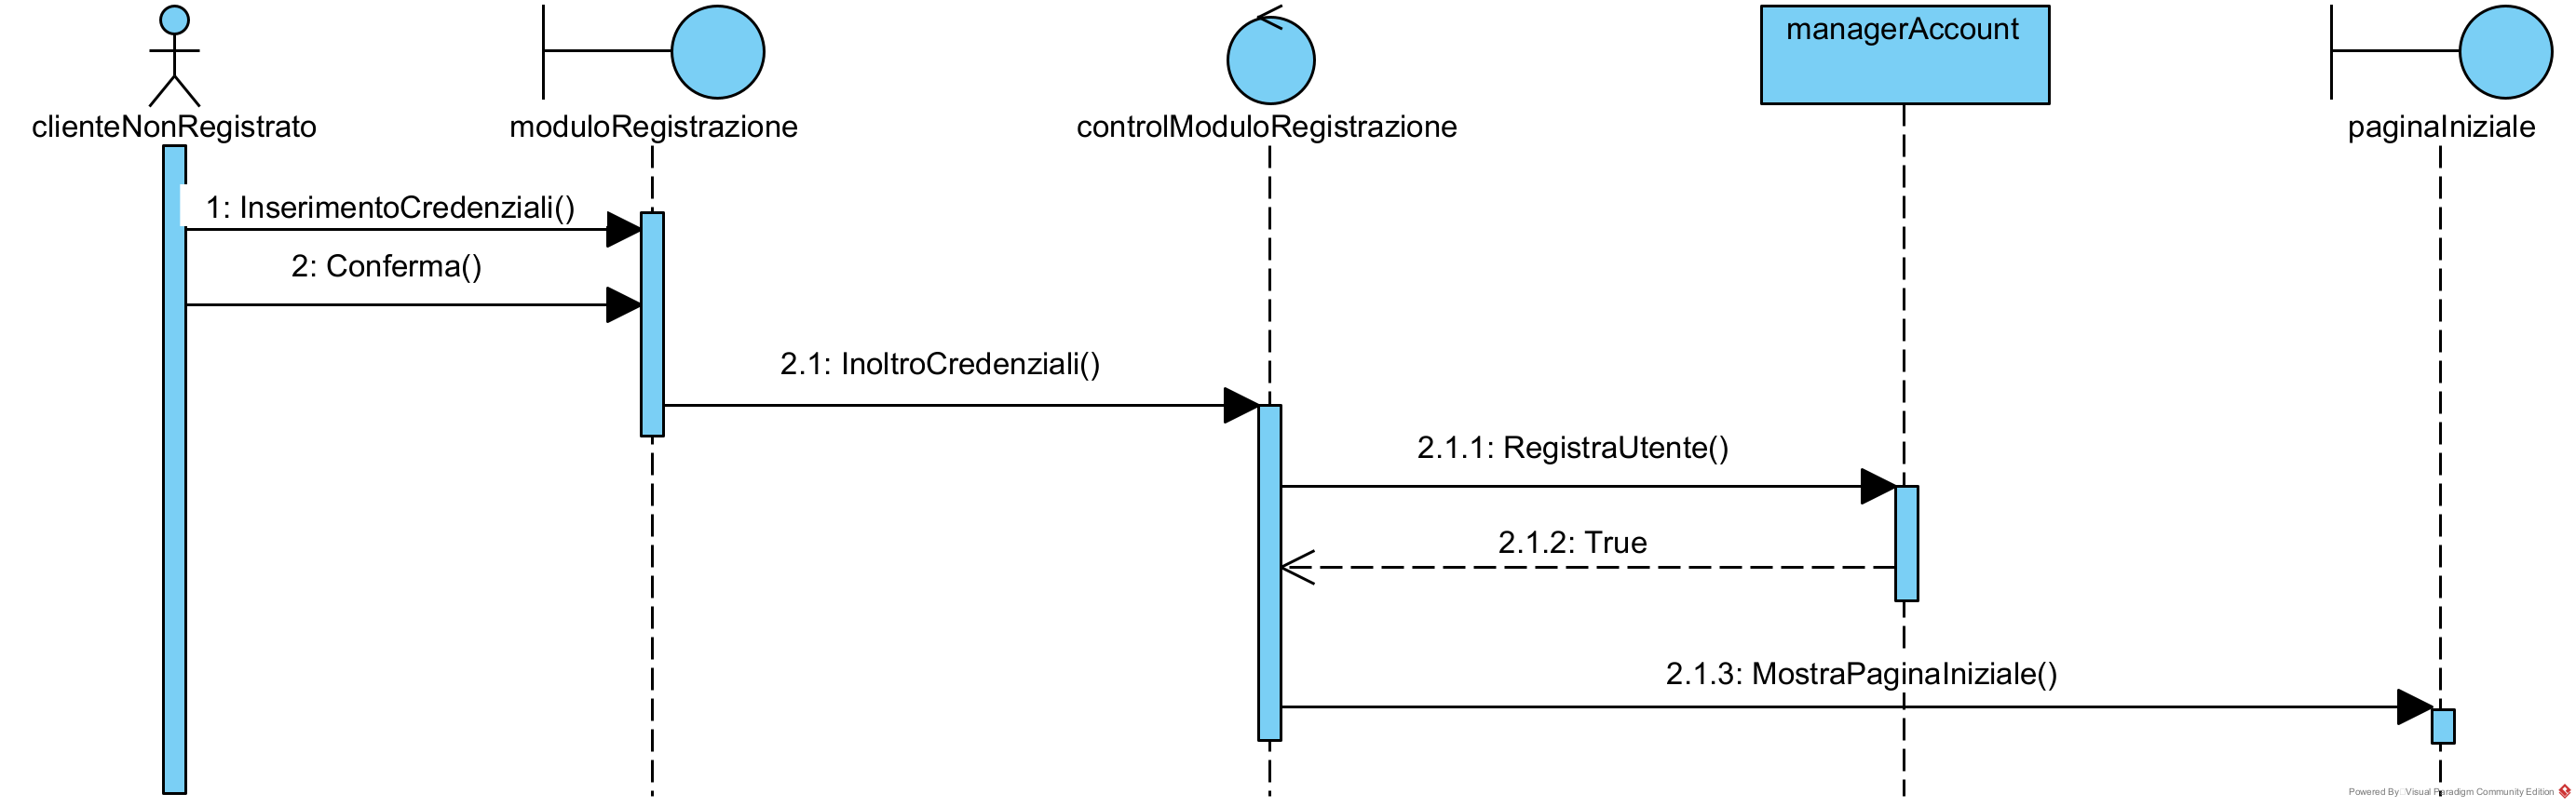
\includegraphics[width=\textwidth]{SequenceDiagram/ClienteRegistrazione}
\end{center}

\begin{enumerate}
\item Un cliente non registrato che visita il sito per la prima volta, una volta deciso di registrarsi, può fare click su ``Registrati'' dalla pagina iniziale.
\item Gli viene presentato un form in cui inserire i dati richiesti per la registrazione, tra cui nome, cognome, email e password.
\item I dati vengono controllati e, se privi di errori, l'utente viene registrato.
\end{enumerate}

\subsubsection{Cliente si autentica}
\label{SD:login}

Fare riferimento a \ref{UC:autenticazione}. \\

\begin{center}
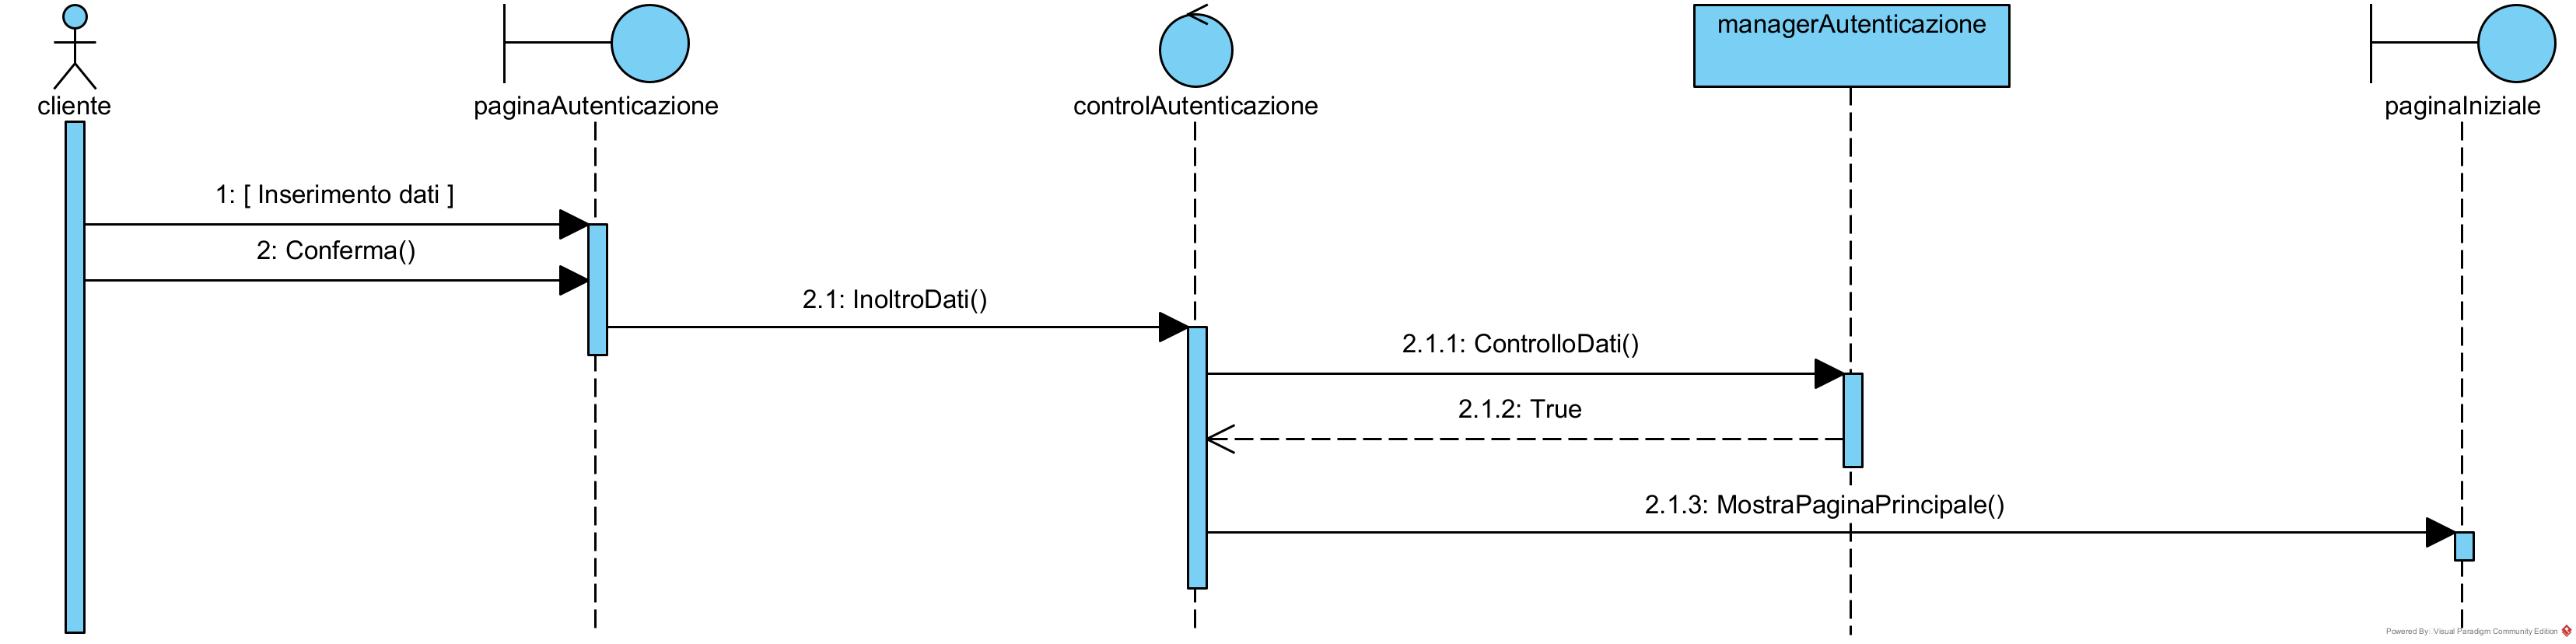
\includegraphics[width=\textwidth]{SequenceDiagram/ClienteAutenticazione}
\end{center}

\begin{enumerate}
\item Dopo la registrazione (\ref{SD:registrazione}), l'utente può usare le credenziali scelte per autenticarsi cliccando sul tasto ``Autenticati''.
\item Gli viene presentato quindi un modulo per l'inserimento di email e password.
\item Se le credenziali sono corrette e corrispondono a quelle memorizzate nel sistema, all'utente viene consentito l'accesso.
\end{enumerate}

\subsubsection{Cliente ricerca un articolo}
\label{SD:ricerca}

\begin{center}
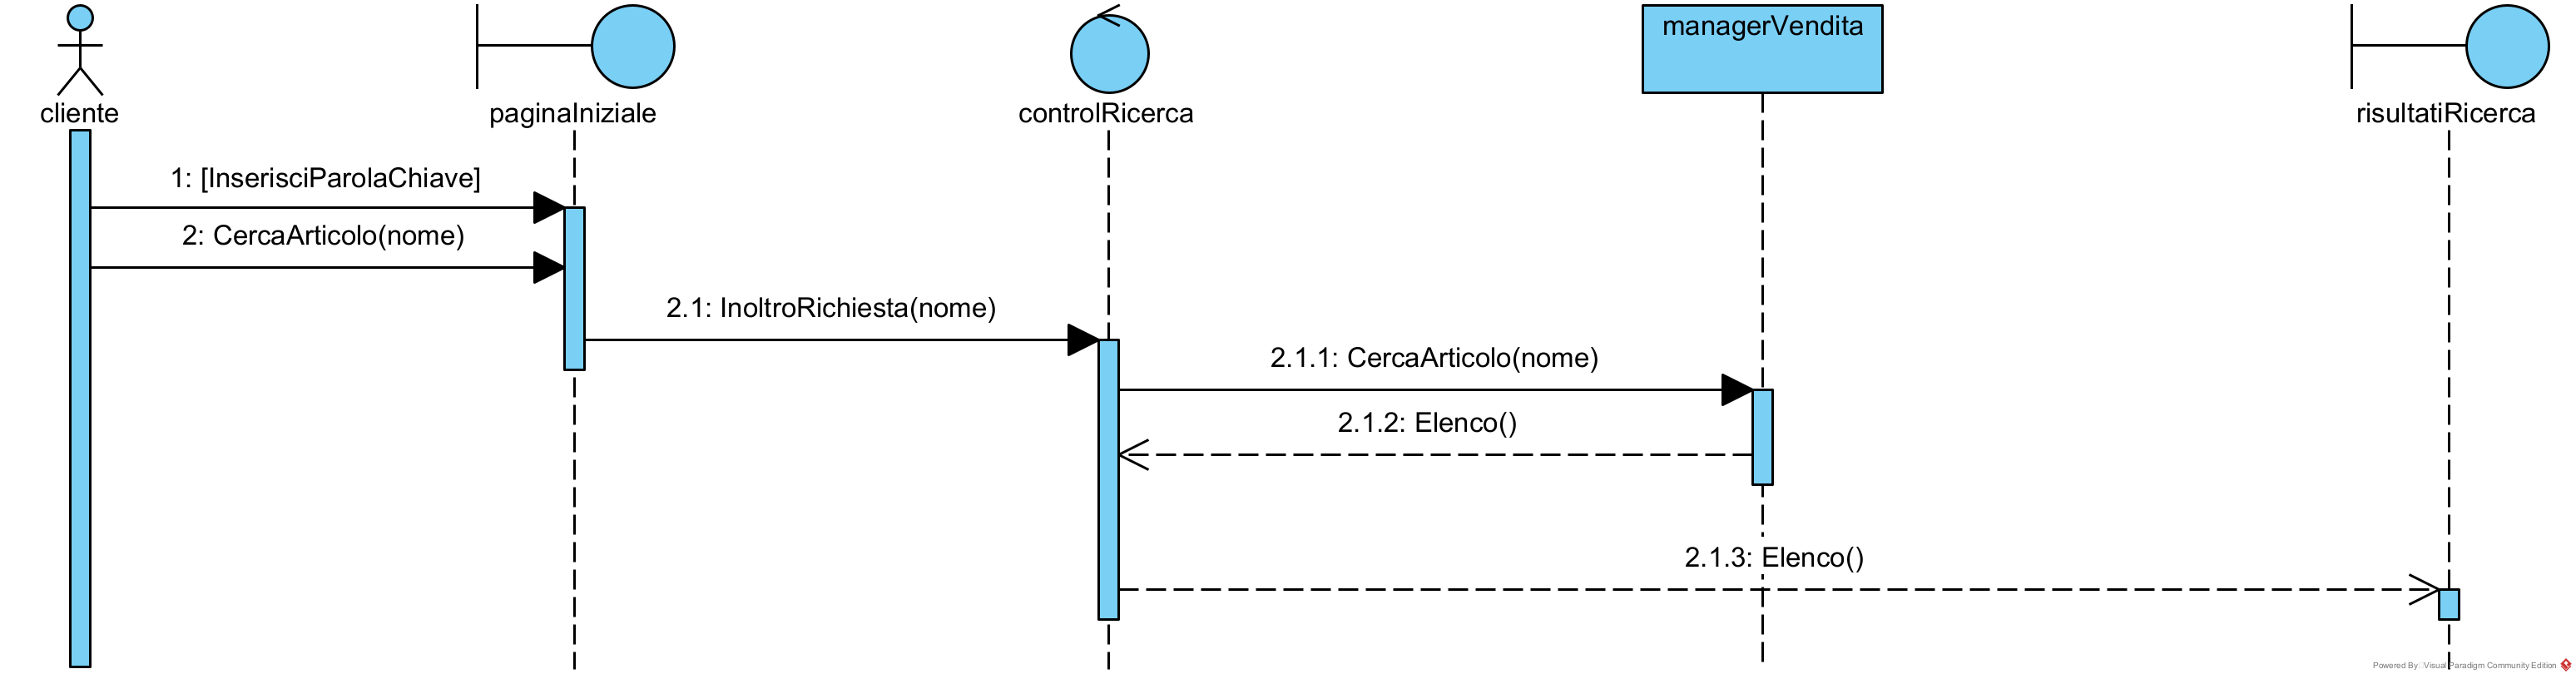
\includegraphics[width=\textwidth]{SequenceDiagram/ClienteArticoloRicerca}
\end{center}

\begin{enumerate}
\item A prescindere dallo stato dell'autenticazione (\ref{SD:login}), all'utente è permesso ricercare articoli nel sito. Usando la barra di ricerca presente nella pagina iniziale, può inserire dei termini da ricercare.
\item Una volta premuto sul tasto ``Cerca'', gli viene presentato un elenco di articoli corrispondenti.
\end{enumerate}

\subsubsection{Cliente visualizza dettagli di un articolo}
\label{SD:dettagli}

\begin{center}
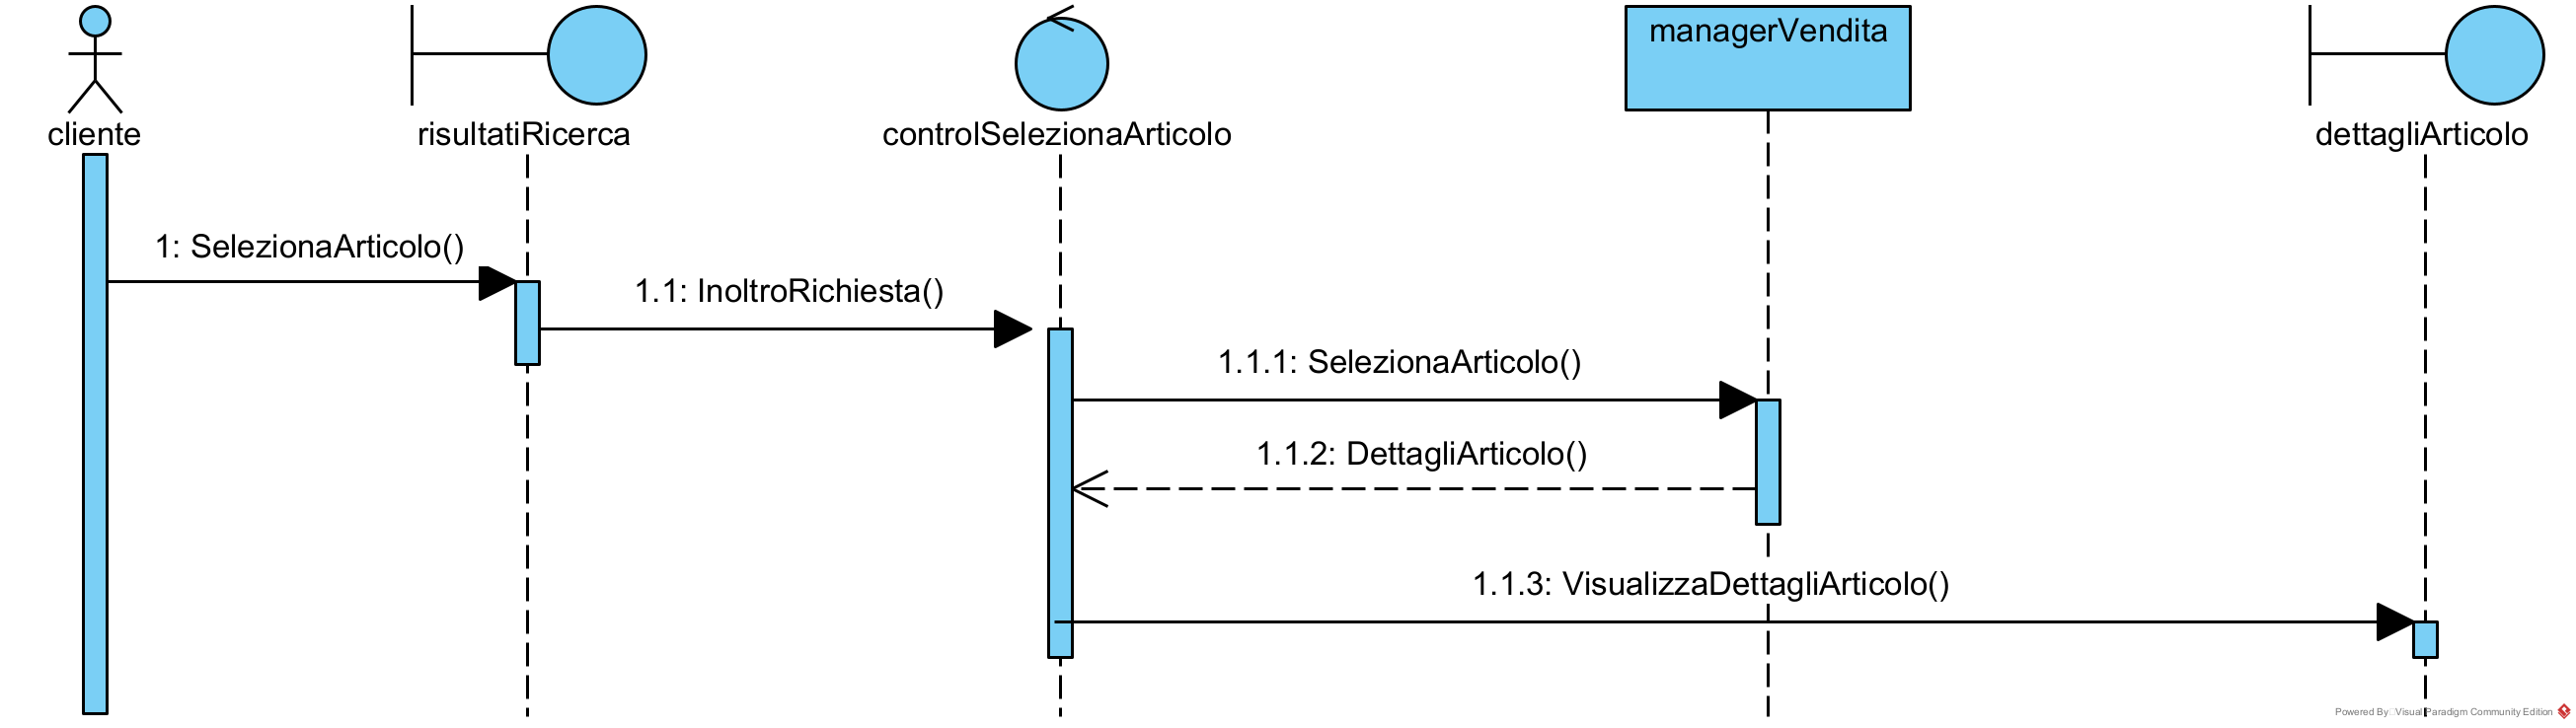
\includegraphics[width=\textwidth]{SequenceDiagram/ClienteArticoloSeleziona}
\end{center}

\begin{enumerate}
\item Dopo aver effettuato una ricerca (\ref{SD:ricerca}), l'utente può scegliere uno degli articoli e selezionarlo per visualizzarne i dettagli.
\item All'utente viene presentata una pagina con i dettagli dell'articolo scelto.
\end{enumerate}

\newpage

\subsubsection{Cliente aggiunge un articolo al carrello}
\label{SD:aggiunta}

Fare riferimento a \ref{UC:carrelloadd}. \\

\begin{center}
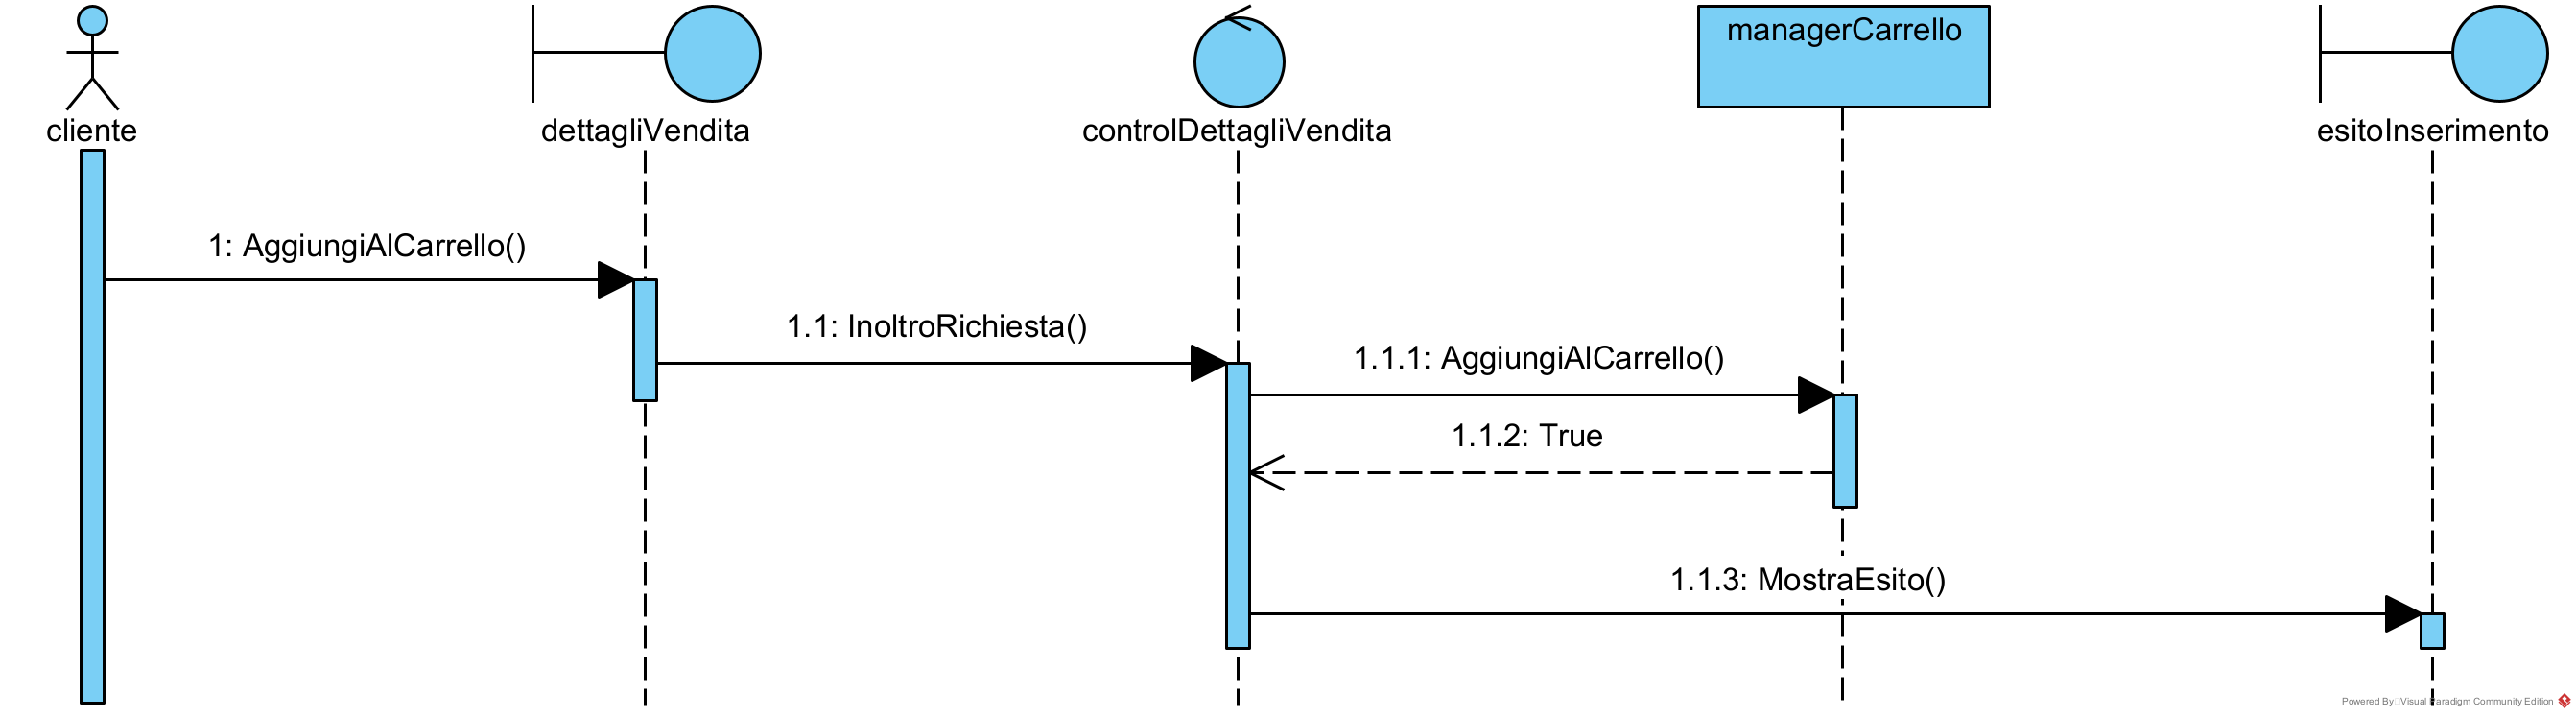
\includegraphics[width=\textwidth]{SequenceDiagram/ClienteCarrelloAggiunge}
\end{center}

\begin{enumerate}
\item Dopo essersi autenticato (\ref{SD:login}) e aver selezionato un articolo (\ref{SD:dettagli}) può aggiungere un articolo al carrello utilizzando il tasto ``Aggiungi al carrello".
\item Una volta premuto, la sua aggiunta viene registrata nel sistema per mantenere il carrello attraverso browser e dispositivi diversi e all'utente viene mostrata una pagina di conferma.
\end{enumerate}

\subsubsection{Cliente rimuove un articolo dal carrello}
\label{SD:rimozione}

Fare riferimento a \ref{UC:carrelloremove}. \\

\begin{center}
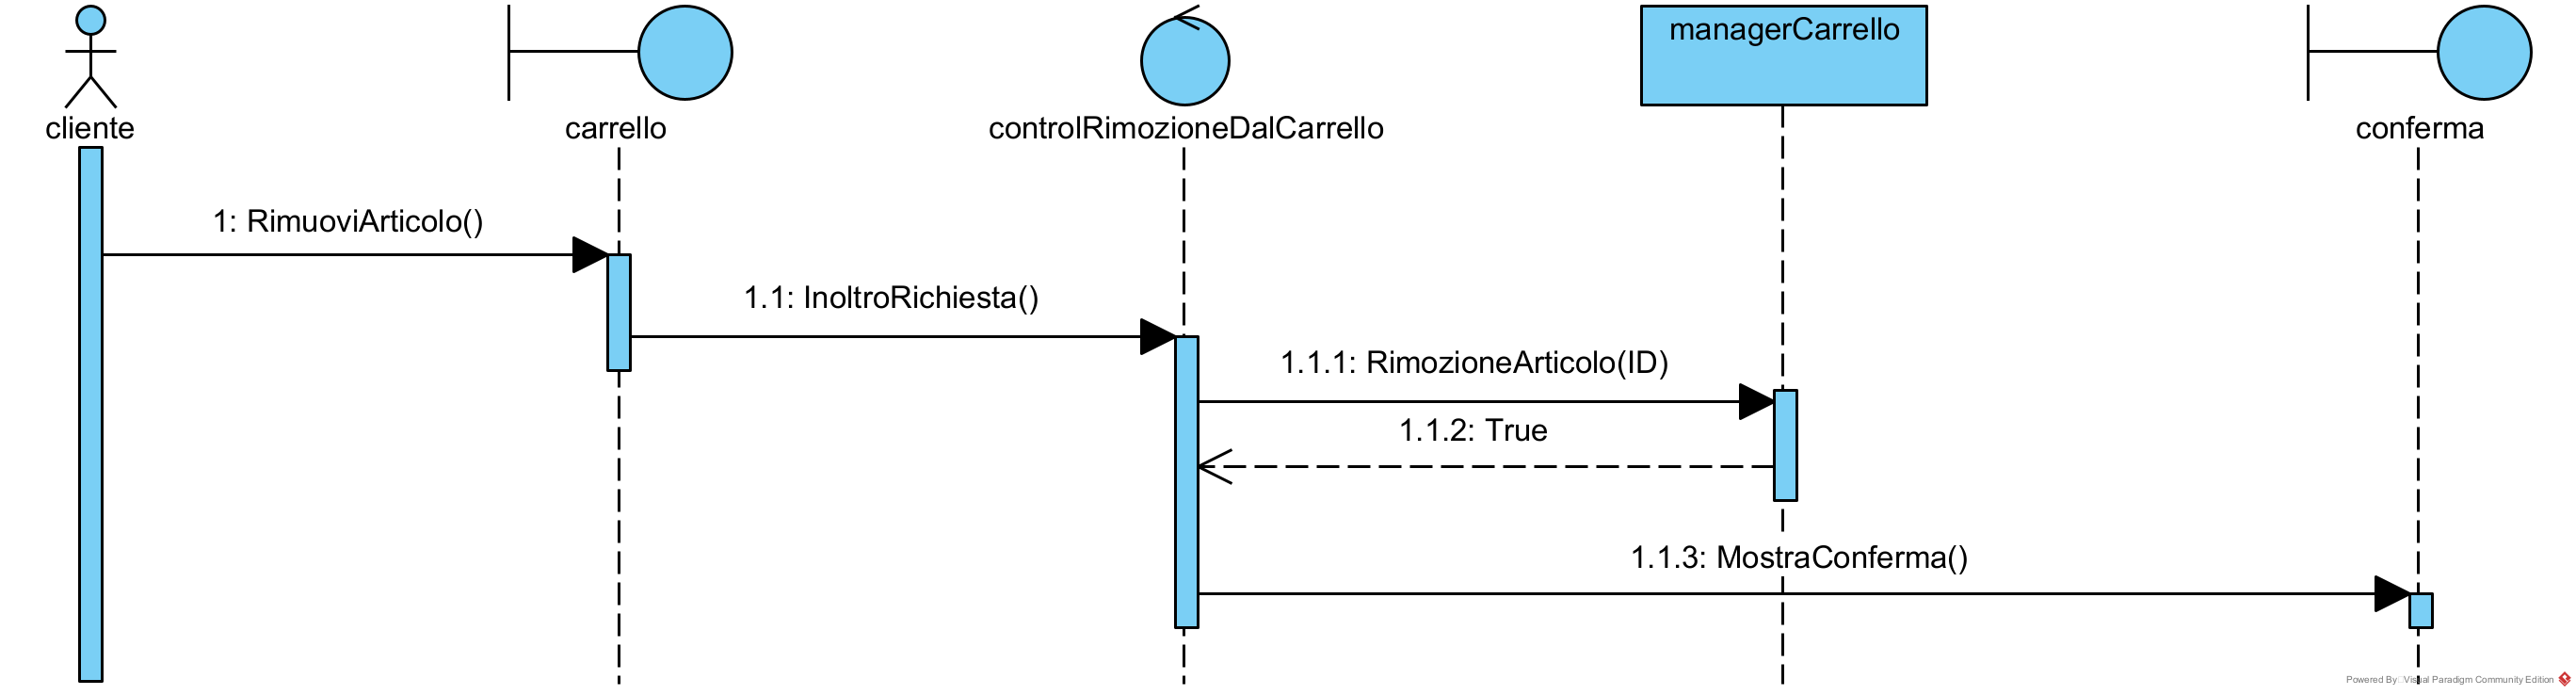
\includegraphics[width=\textwidth]{SequenceDiagram/ClienteCarrelloRimuove}
\end{center}

\begin{enumerate}
\item Dopo aver aggiunto un articolo al carrello (\ref{SD:aggiunta}), all'utente è consentita la rimozione degli articoli dal carrello usando il tasto ``Rimuovi".
\item Una volta premuto, la sua modifica viene registrata e all'utente viene mostrata una pagina di conferma.
\end{enumerate}

\newpage

\subsubsection{Cliente acquista articoli}
\label{SD:acquista}

\begin{center}
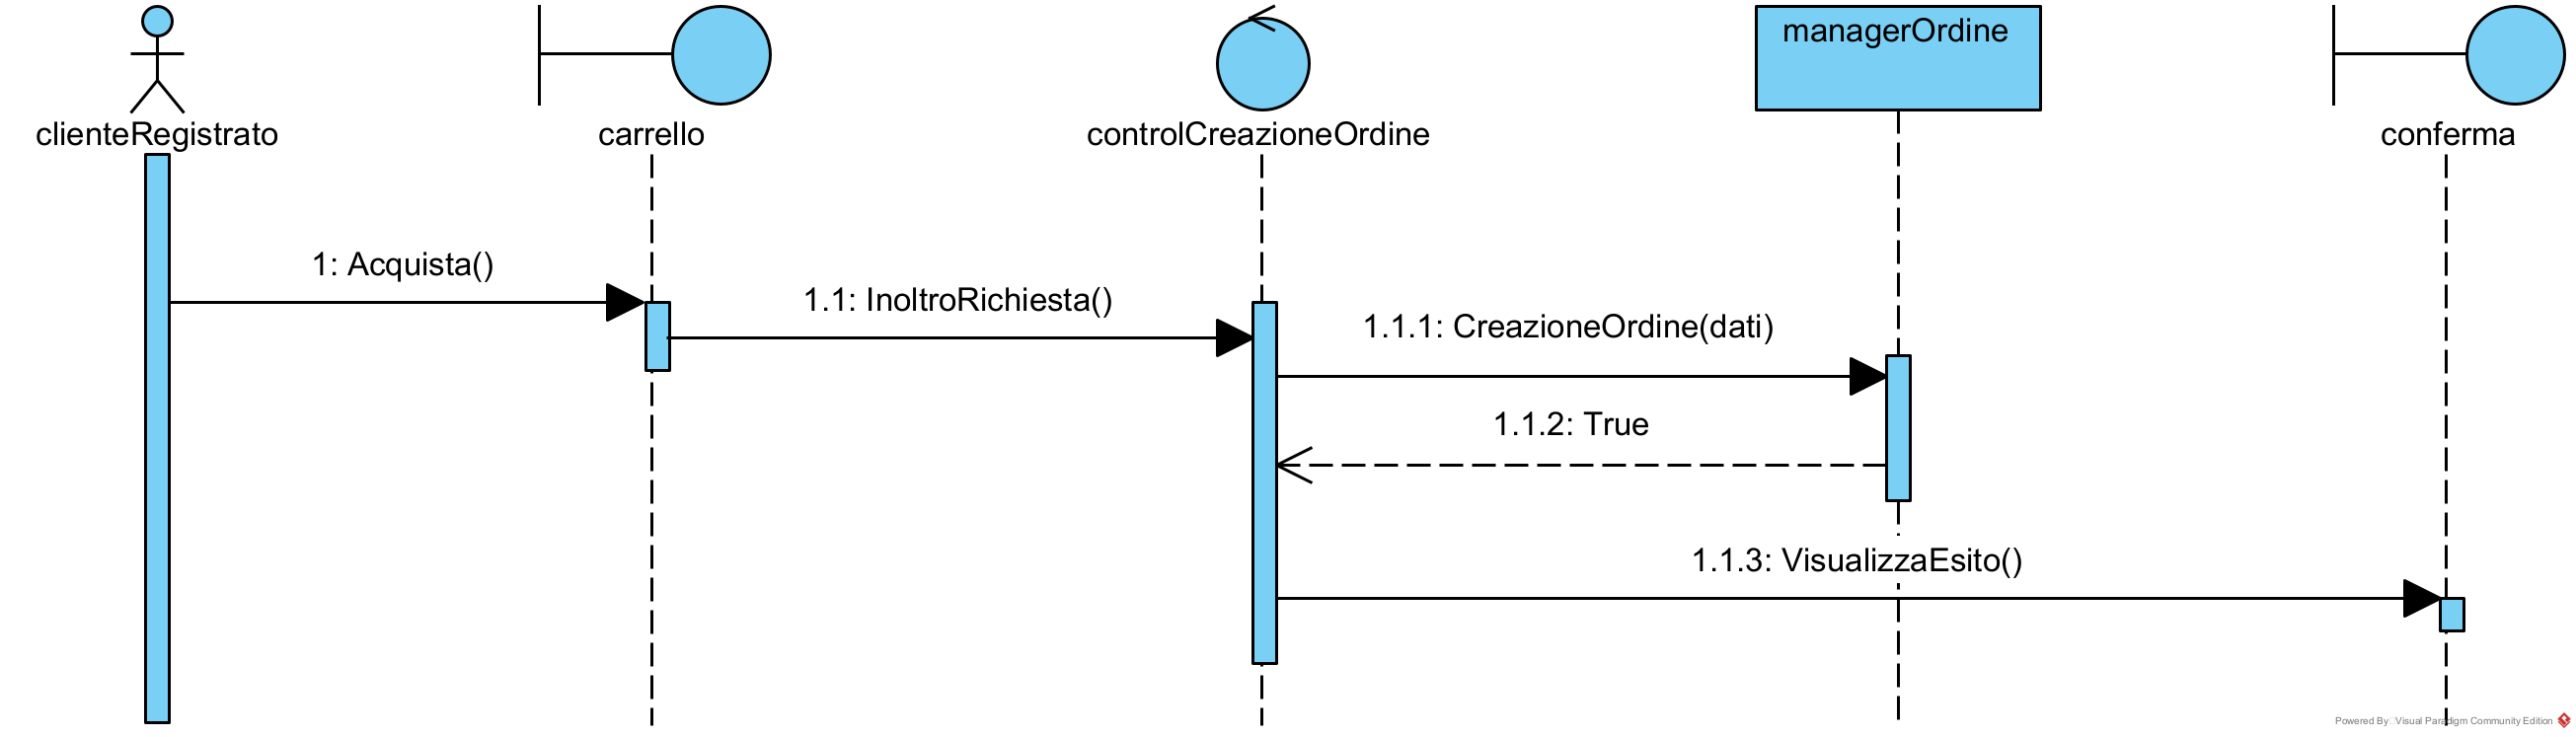
\includegraphics[width=\textwidth]{SequenceDiagram/ClienteArticoloAcquista}
\end{center}

\begin{enumerate}
\item Dopo aver aggiunto almeno un articolo al carrello (\ref{SD:aggiunta}), l'utente ha la possibilità di ordinare gli articoli nel carrello stesso.
\item Dopo aver premuto su ``Acquista'', gli viene chiesta un'ulteriore conferma in una pagina contenente tutte le informazioni relative all'ordine.
\item Una volta ricevuta la conferma, l'ordine viene registrato ed è visualizzabile da un magazziniere  (\ref{SD:magazzinierespedisce}).
\end{enumerate}

\subsubsection{Cliente annulla ordine}
\label{SD:annull}

Fare riferimento a \ref{UC:annullamento}. \\

\begin{center}
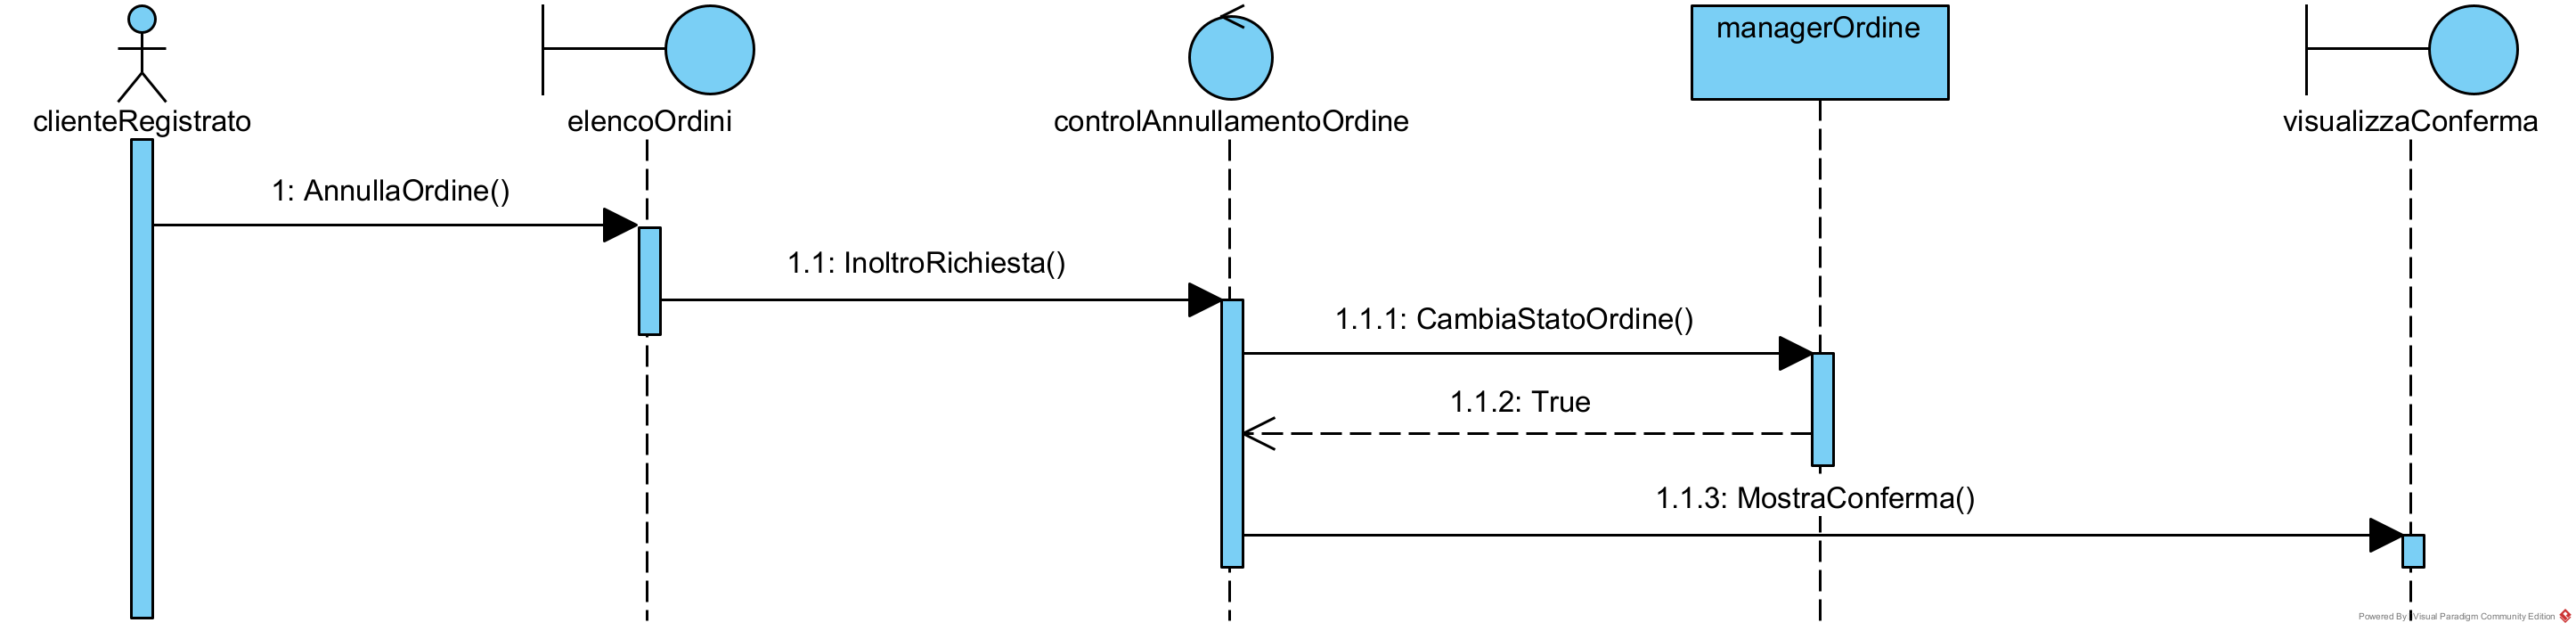
\includegraphics[width=\textwidth]{SequenceDiagram/ClienteOrdineAnnulla}
\end{center}

\begin{enumerate}
\item Dopo aver effettuato un ordine e prima che venga spedito, ad un cliente è permesso annullare un ordine.
\item Dall'elenco degli ordini ha la possibilità di richiedere l'annullamento. Se lo stato nel sistema è ancora ``Non spedito'' l'ordine viene effettivamente annullato immediatamente e sparirà dalla visualizzazione dei magazzinieri (\ref{SD:magazzinierespedisce}). In caso contrario, non è possibile annullarlo.
\end{enumerate}

\newpage

\subsubsection{Cliente visualizza elenco vendite}
\label{SD:elencovendite}

\begin{center}
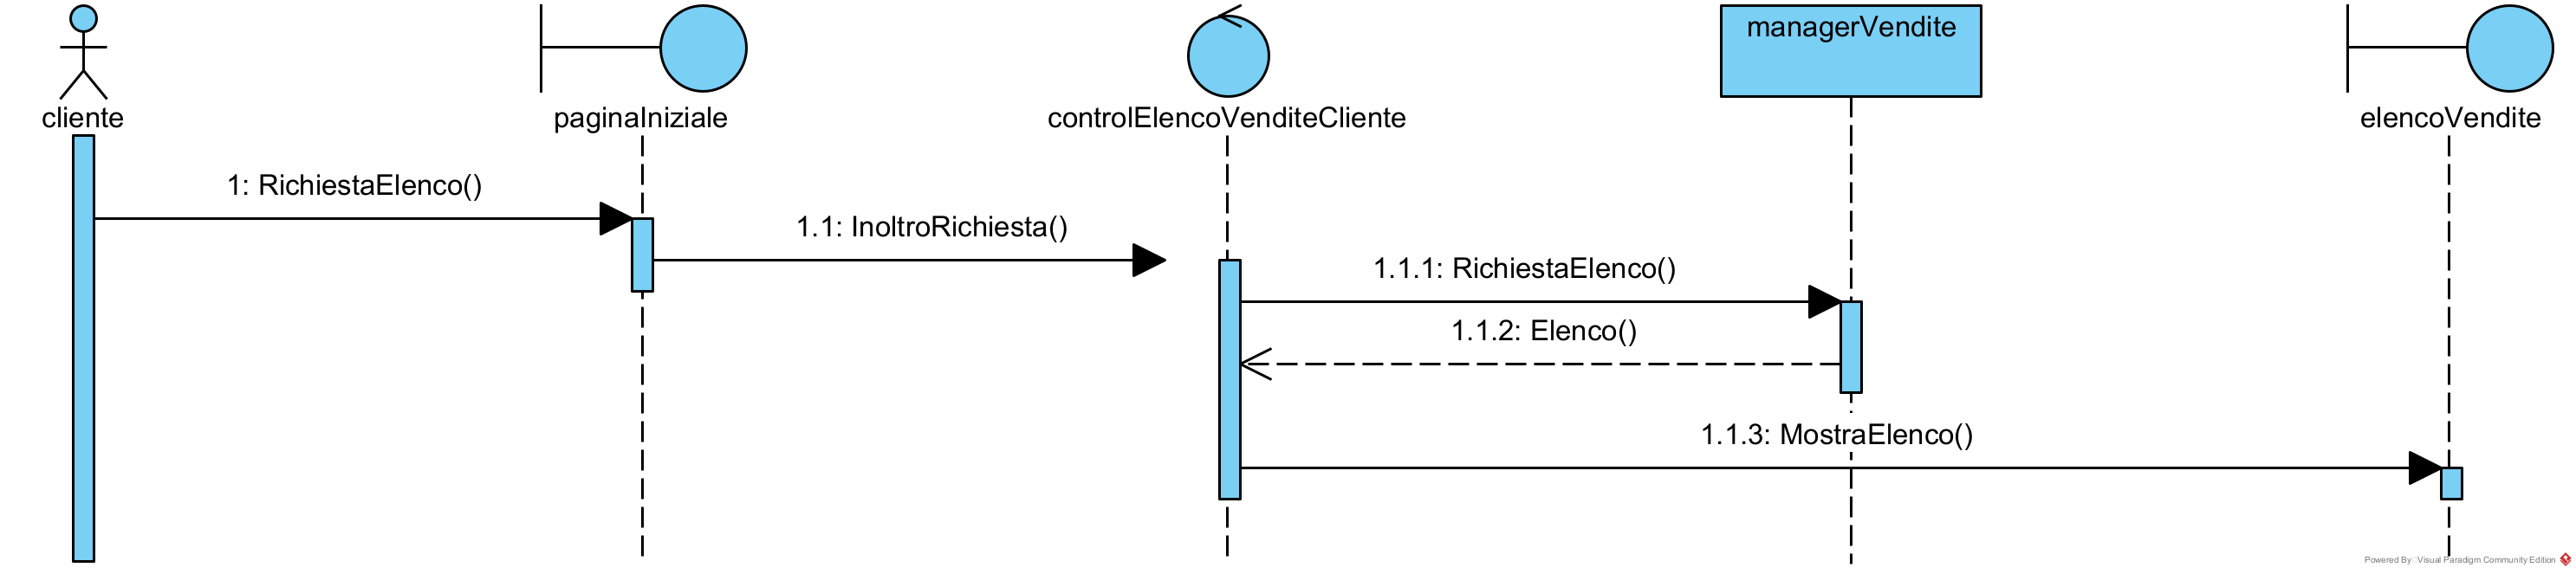
\includegraphics[width=\textwidth]{SequenceDiagram/ClienteVenditaElenco}
\end{center}

\begin{enumerate}
\item Dalla pagina iniziale, l'utente può selezionare la voce ``Area venditori" per visualizzare la pagina dedicata alla gestione delle vendite.
\item Al caricamento della pagina, vengono caricate le vendite create più recentemente, ovvero nei 60 giorni precedenti.
\end{enumerate}

\subsubsection{Cliente vende articolo}
\label{SD:creazionevendita}

Fare riferimento a \ref{UC:salesnew}. \\

\begin{center}
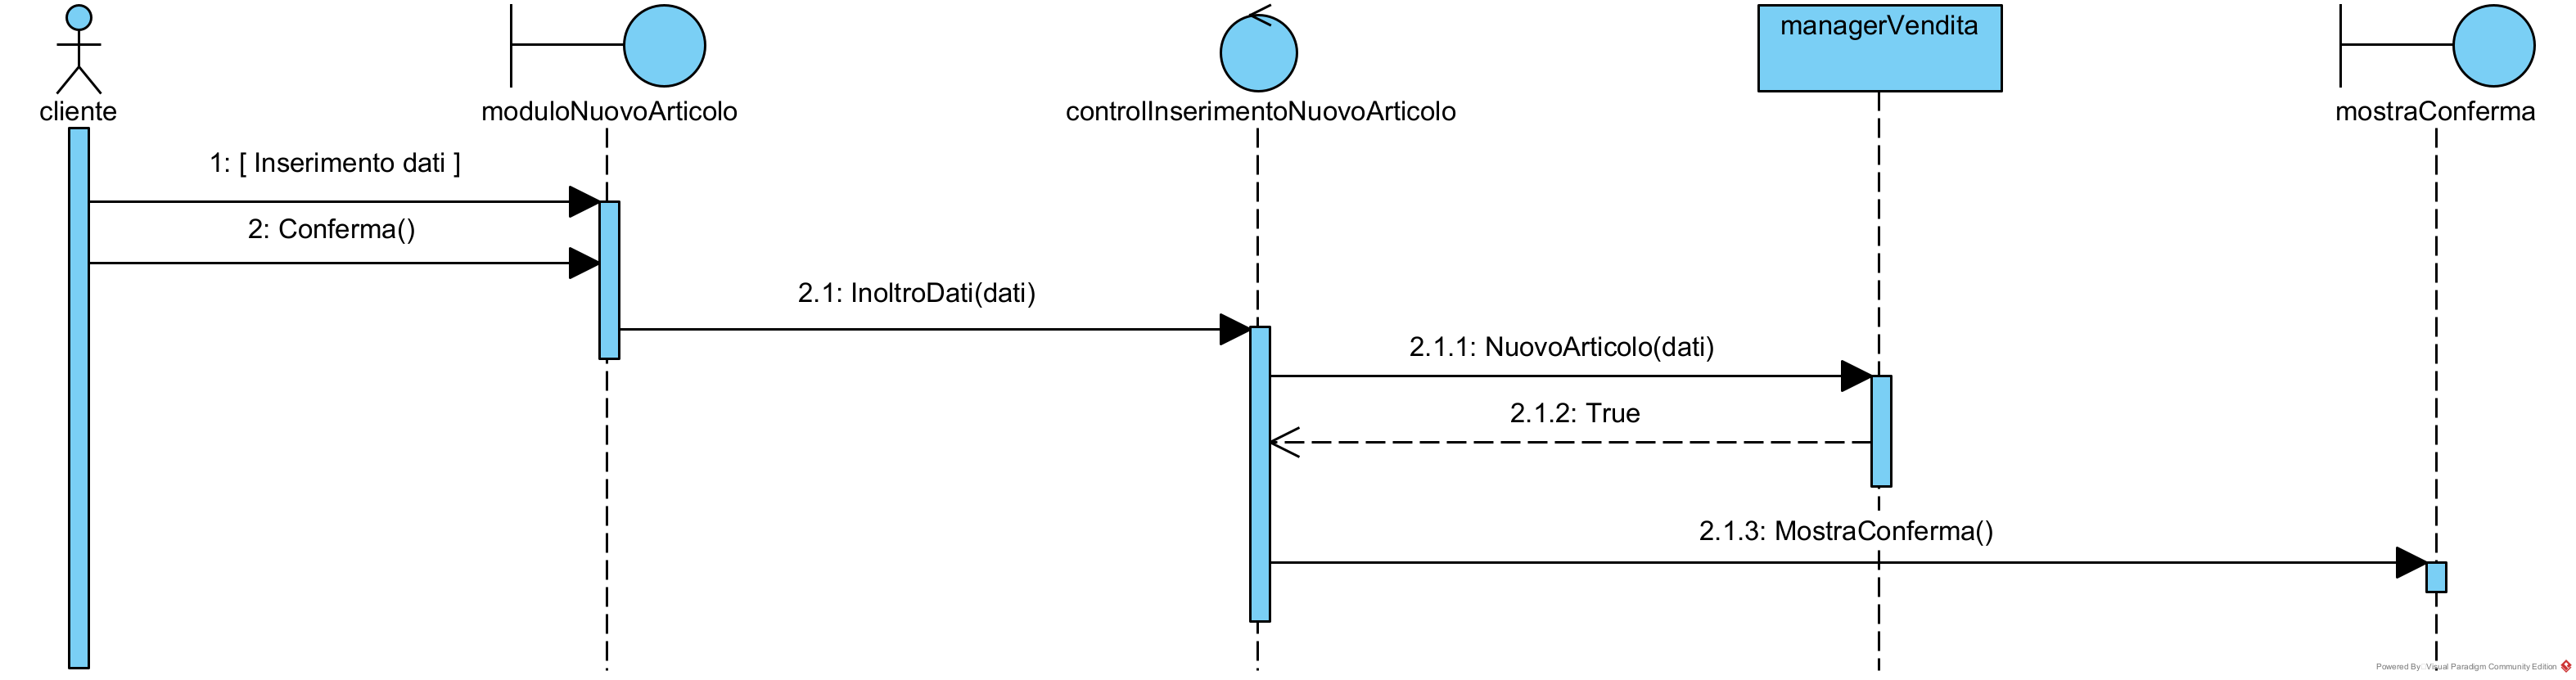
\includegraphics[width=\textwidth]{SequenceDiagram/ClienteVenditaCrea}
\end{center}

\begin{enumerate}
\item Dall'elenco delle vendite (\ref{SD:elencovendite}), è sufficiente utilizzare il tasto ``Inserisci nuova vendita".
\item Viene richiesto all'utente di compilare un modulo con i dati necessari come nome, prezzo, descrizione, quantità disponibile e di inserire almeno 3 foto del prodotto.
\item La nuova vendita viene quindi inserita nel sistema in uno stato di attesa finché un centralinista non verificherà le informazioni della vendita (\ref{SD:centralinistaautorizza}).
\end{enumerate}

\subsubsection{Cliente seleziona vendita}
\label{SD:selezionavenditacliente}

\begin{center}
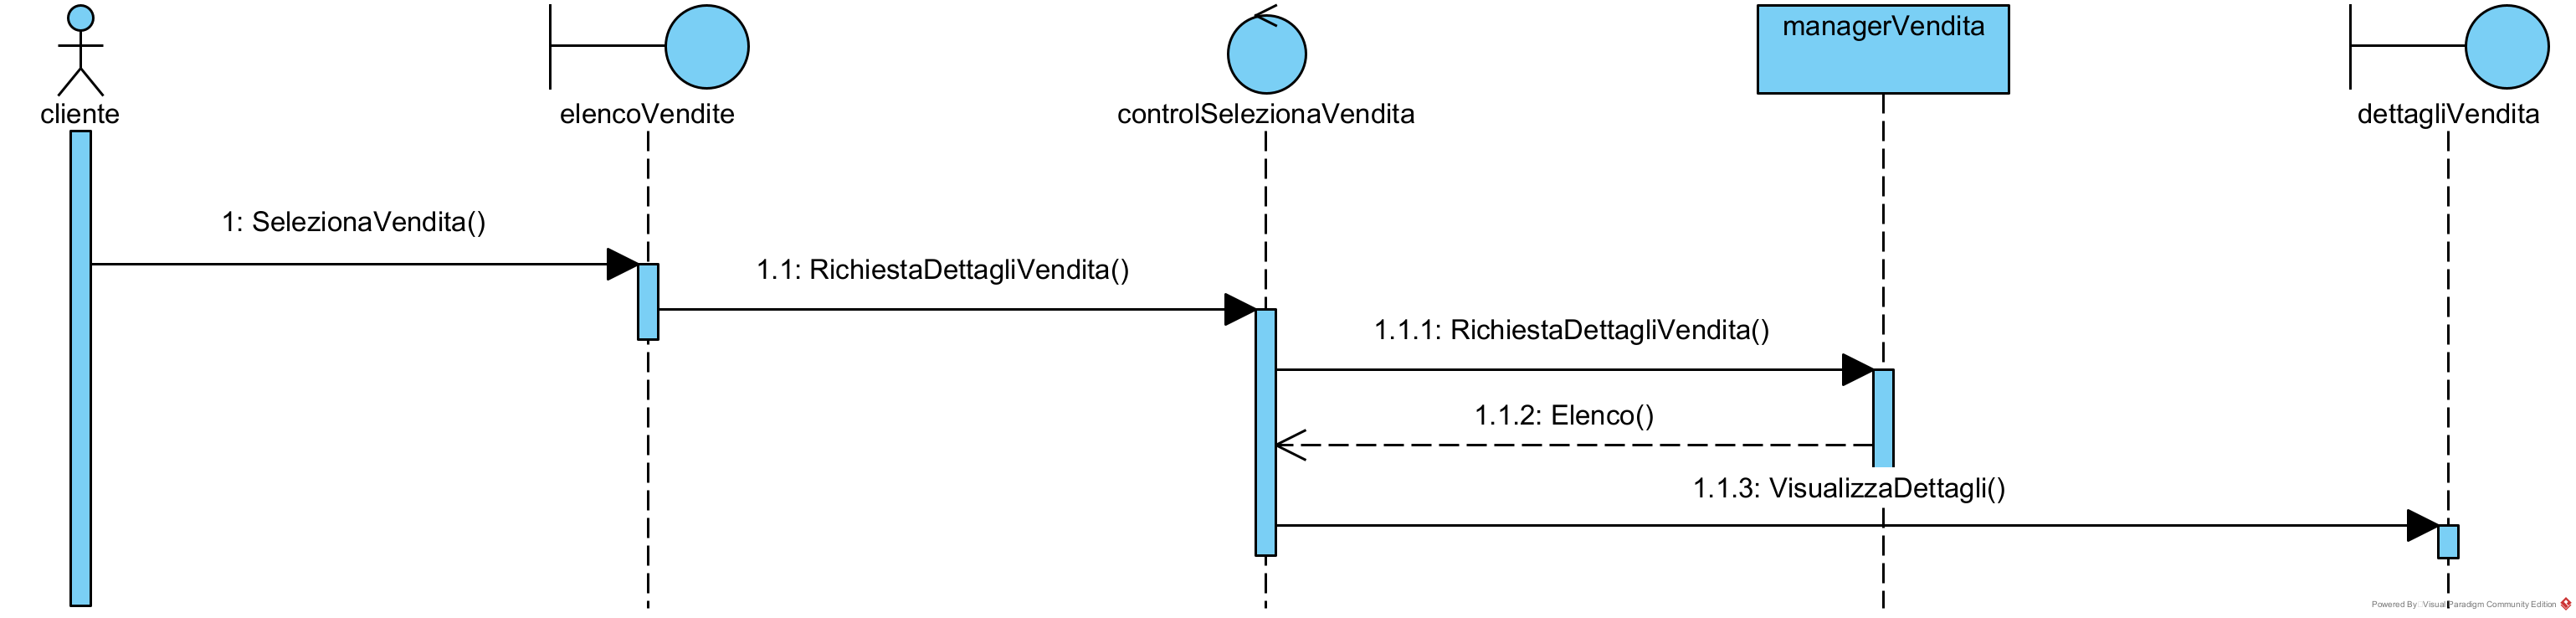
\includegraphics[width=\textwidth]{SequenceDiagram/ClienteVenditaSeleziona}
\end{center}

\begin{enumerate}
\item Dall'elenco delle vendite (\ref{SD:elencovendite}), il cliente ne può selezionare una per visualizzarne i dettagli.
\item Gli viene mostrata una pagina con informazioni sulla vendita come la quantità di articoli venduti e il ricavato totale.
\end{enumerate}

\subsubsection{Cliente modifica vendita}
\label{SD:modificavendita}

\begin{center}
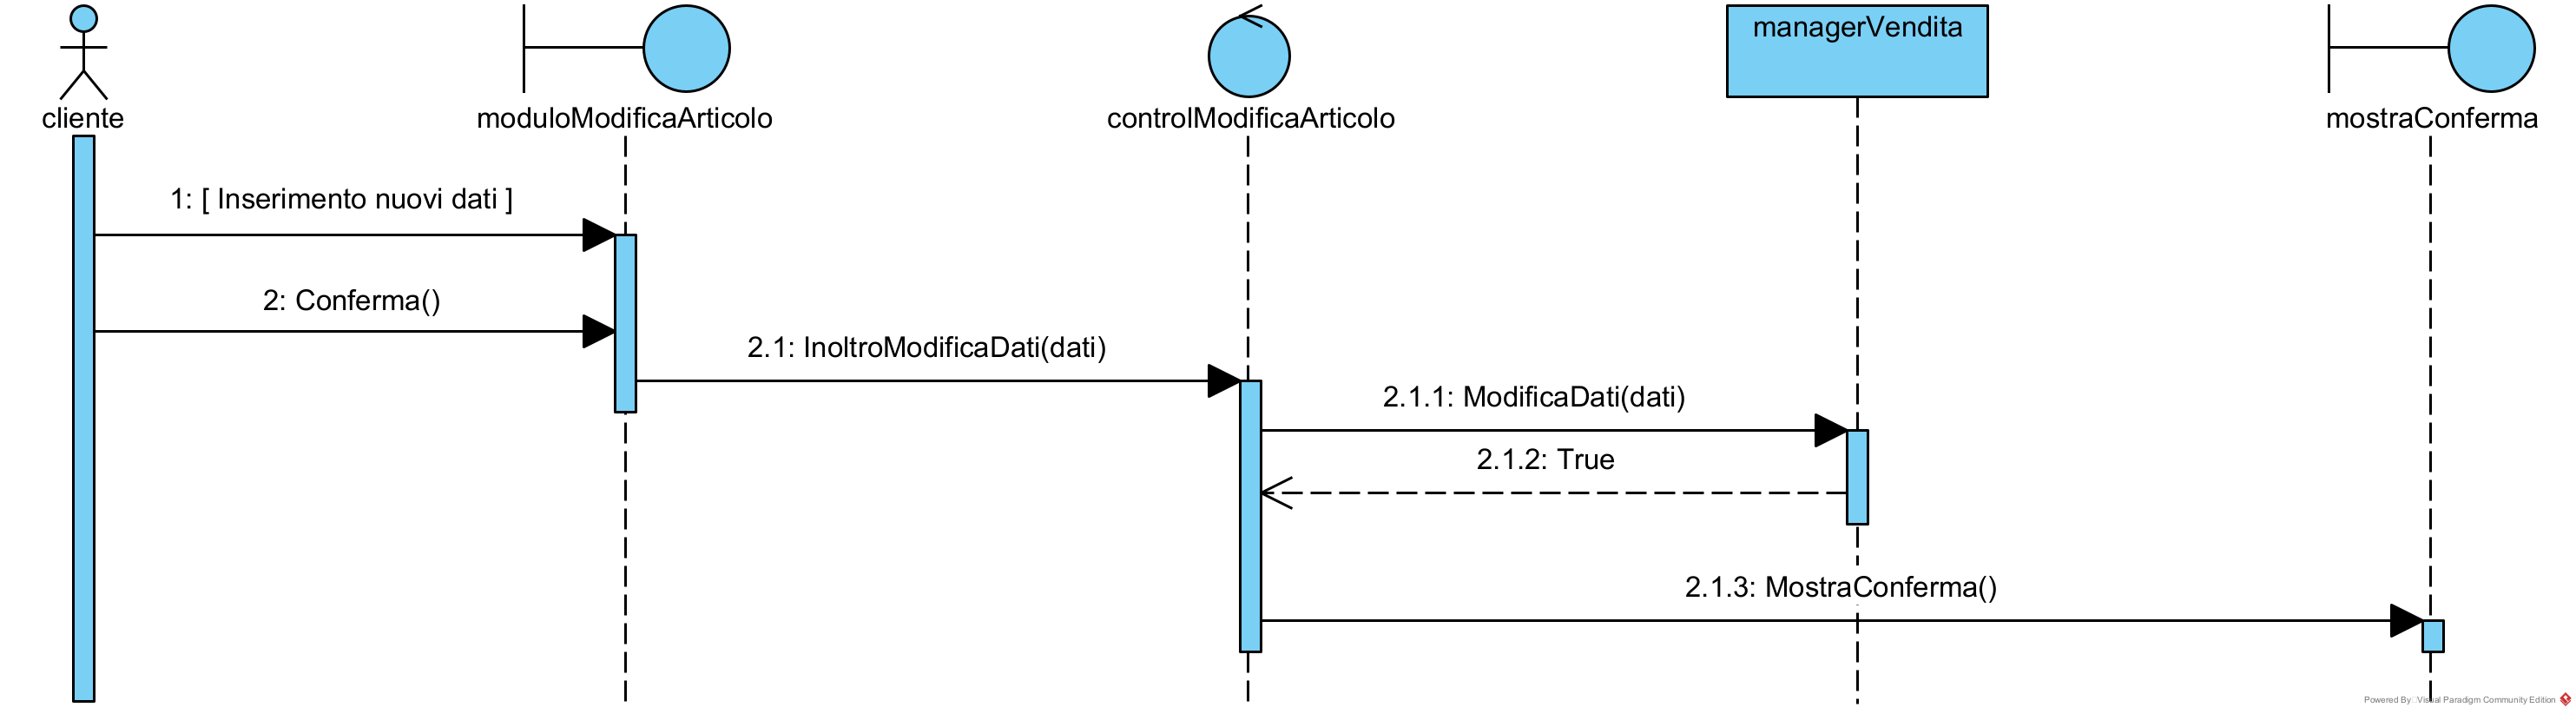
\includegraphics[width=\textwidth]{SequenceDiagram/ClienteVenditaModifica}
\end{center}

\begin{enumerate}
\item Nella pagina dei dettagli di una vendita, se lo stato è ``In vendita", è presente anche un tasto ``Modifica vendita".
\item L'utente può cliccarlo per visualizzare un modulo per la modifica della vendita. 
\item La vendita torna quindi in uno stato di attesa finché un centralinista non verificherà i dati inseriti (\ref{SD:centralinistaautorizza}).
\end{enumerate}

\subsubsection{Cliente annulla vendita}
\label{SD:annullavendita}

\begin{center}
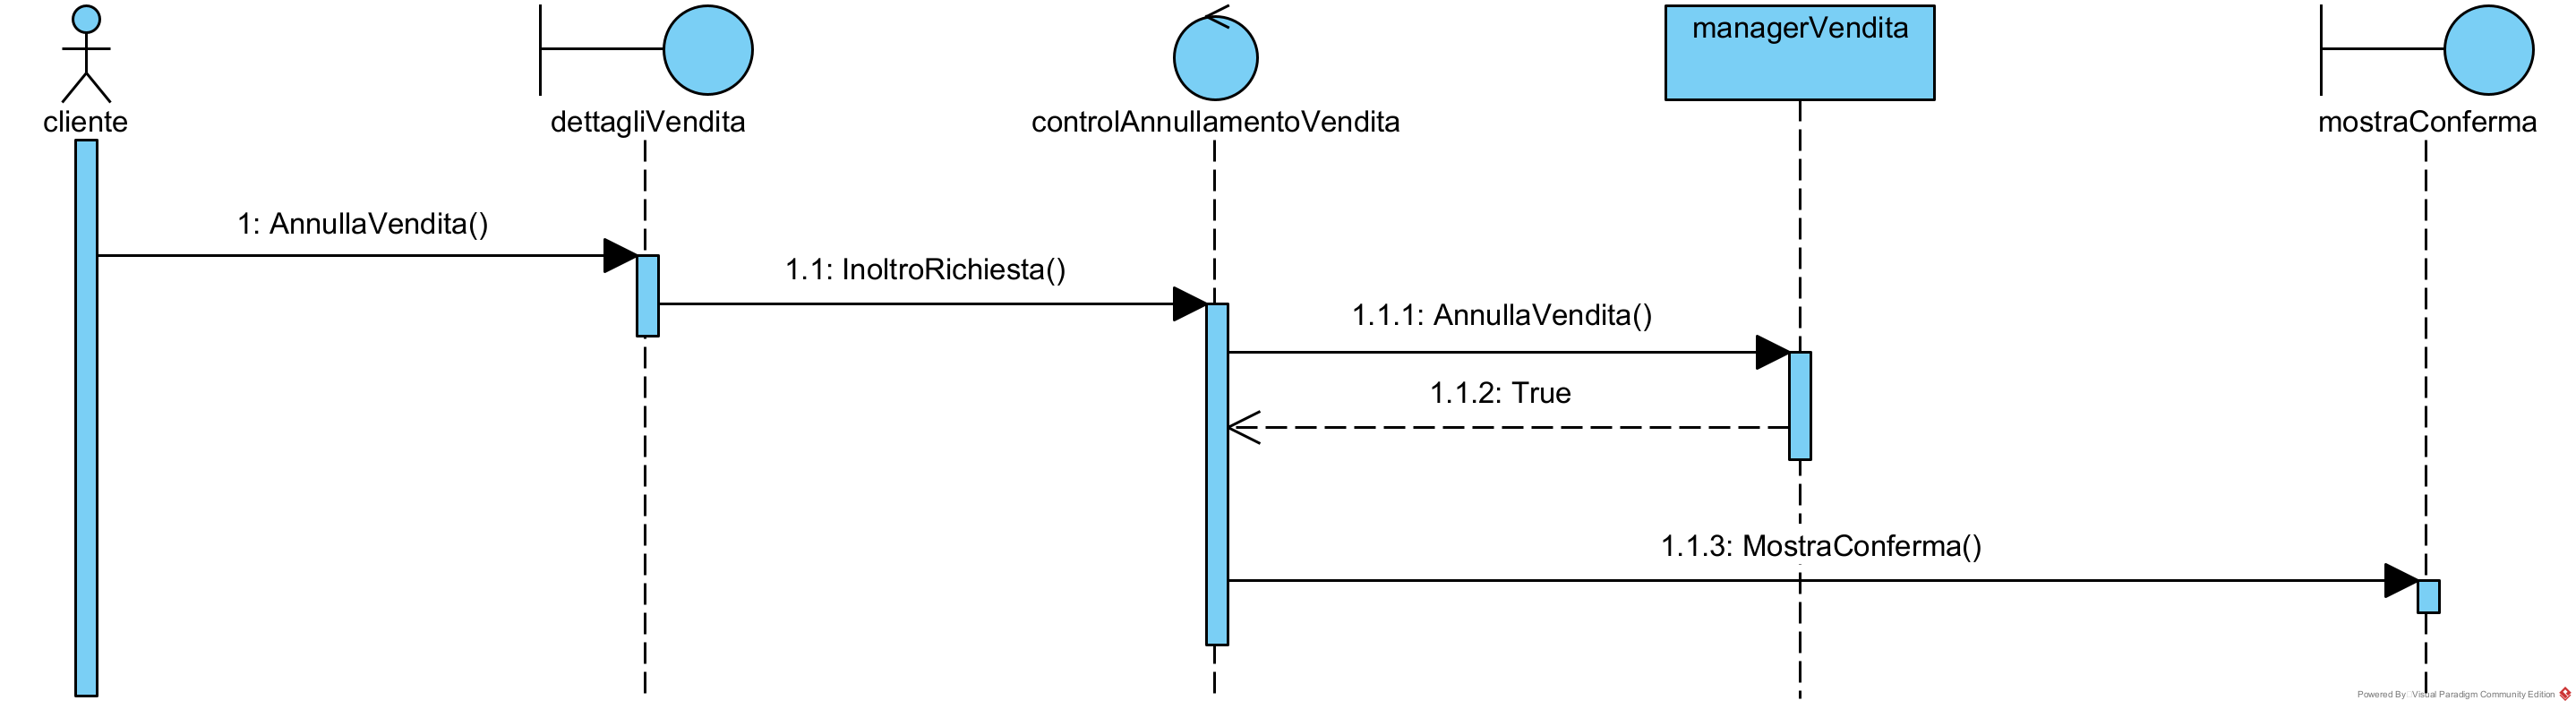
\includegraphics[width=\textwidth]{SequenceDiagram/ClienteVenditaAnnulla}
\end{center}

\begin{enumerate}
\item Dopo aver creato una vendita (\ref{SD:creazionevendita}) e finché lo stato è ``In vendita", all'utente è concessa la possibilità di annullare una vendita.
\item Dall'elenco delle vendite è presente quindi un tasto ``Annulla vendita".
\item All'utente viene mostrata una pagina di conferma.
\end{enumerate}

\newpage

\subsubsection{Cliente elenca ticket}
\label{SD:elencoticket}
Fare riferimento a \ref{UC:ticketlist}. \\

\begin{center}
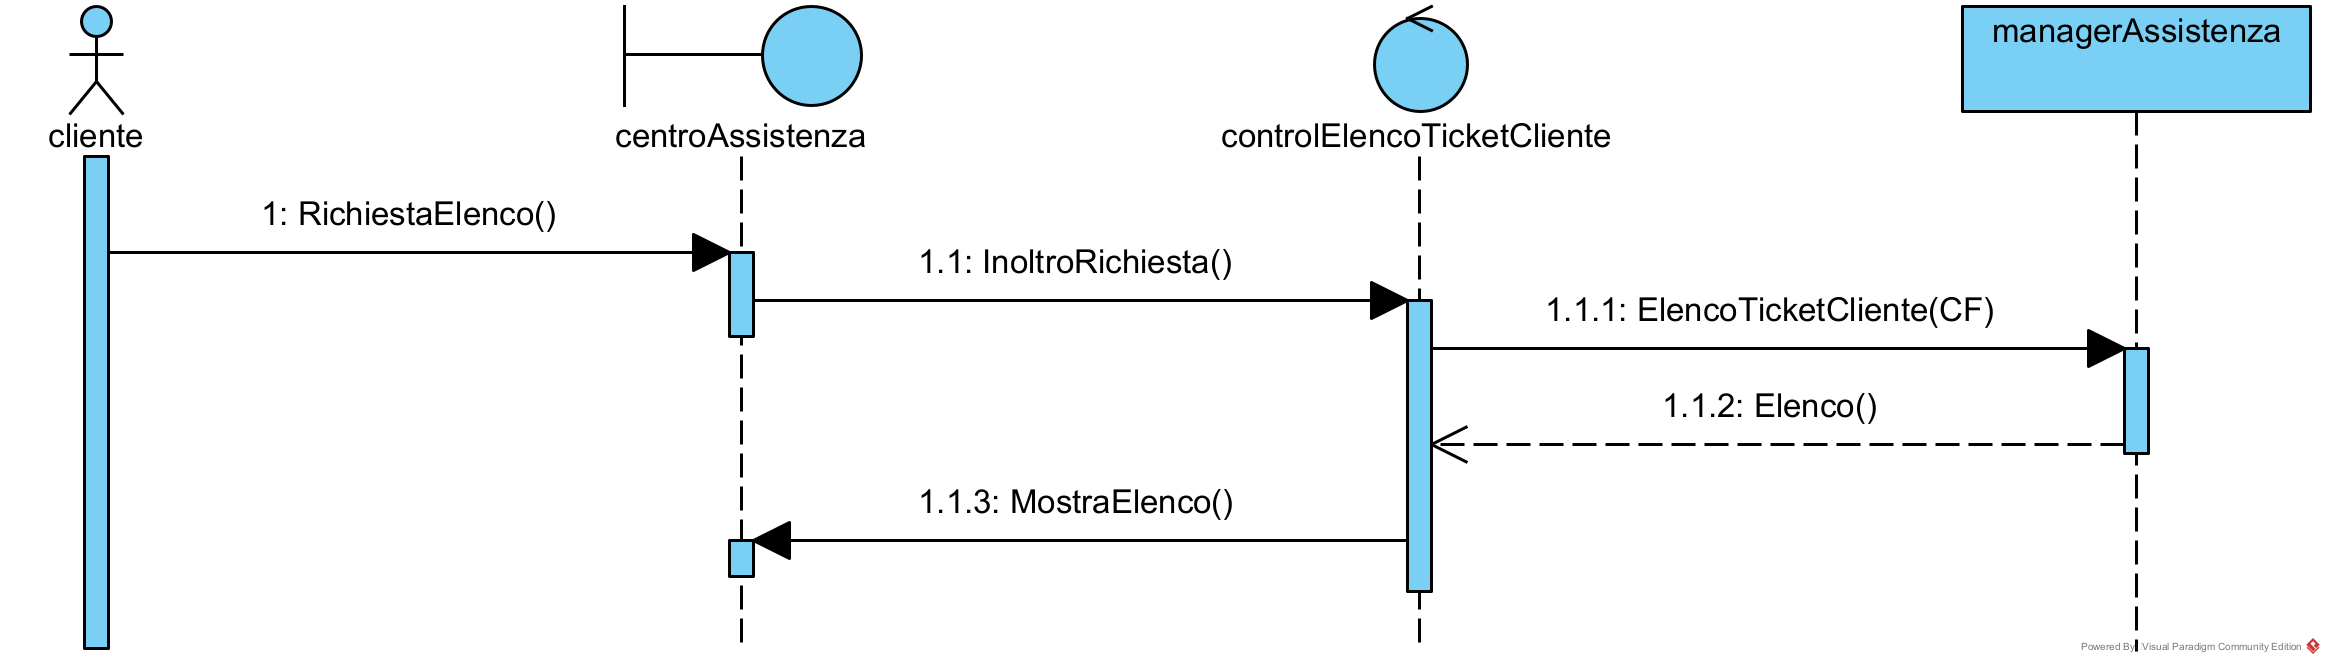
\includegraphics[width=\textwidth]{SequenceDiagram/ClienteTicketElenco}
\end{center}

\begin{enumerate}
\item Un utente autenticato (\ref{SD:login}) che si trova nella pagina iniziale può utilizzare la funzione ``Assistenza Clienti".
\item Gli viene quindi mostrato l'elenco dei ticket attualmente in attesa di risoluzione e che non sono attualmente visualizzati da altri centralinisti.
\end{enumerate}

\subsubsection{Cliente apre ticket}
\label{SD:aperturaticket}

\begin{center}
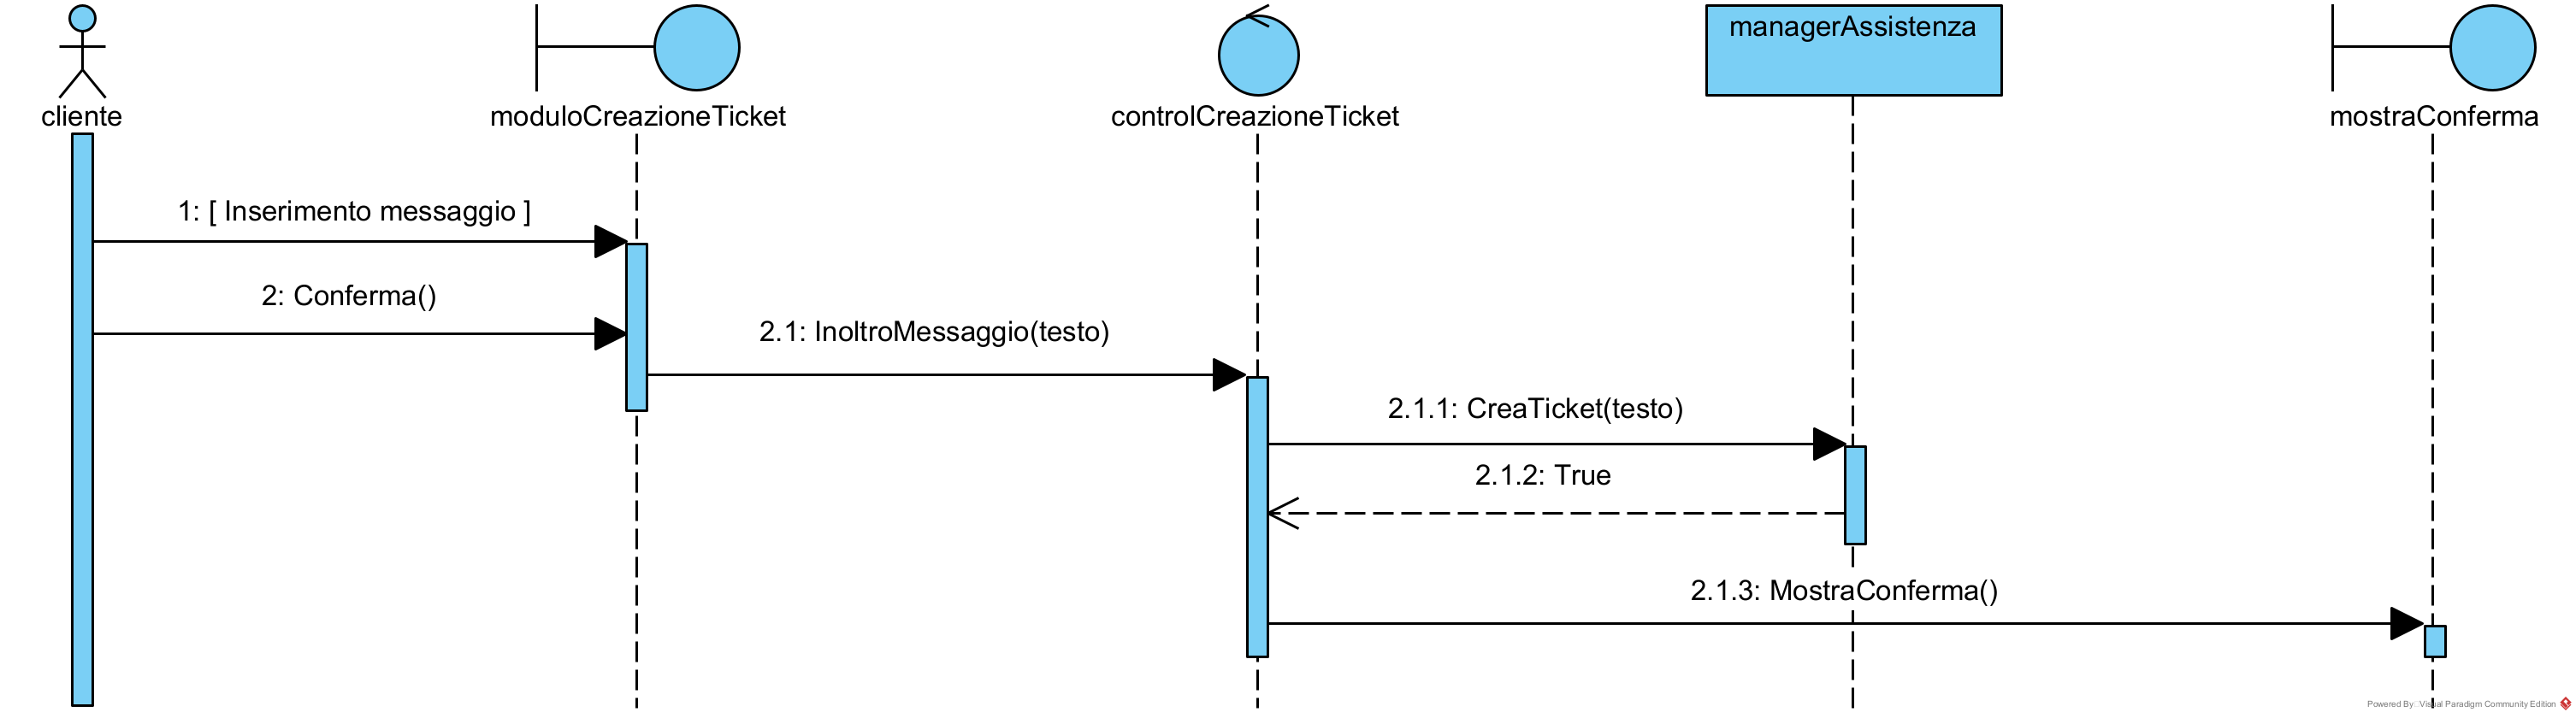
\includegraphics[clip,width=\textwidth]{SequenceDiagram/ClienteTicketCreazione}
\end{center}

\begin{enumerate}
\item Dall'elenco dei ticket (\ref{SD:elencoticket}), l'utente usa la funzione ``Crea Ticket".
\item Gli viene mostrato un modulo per l'inserimento del messaggio per la scelta della tipologia del problema.
\item All'utente viene mostrata una conferma.
\end{enumerate}

\subsubsection{Cliente seleziona un ticket}
\label{SD:selezioneticketcliente}

\begin{center}
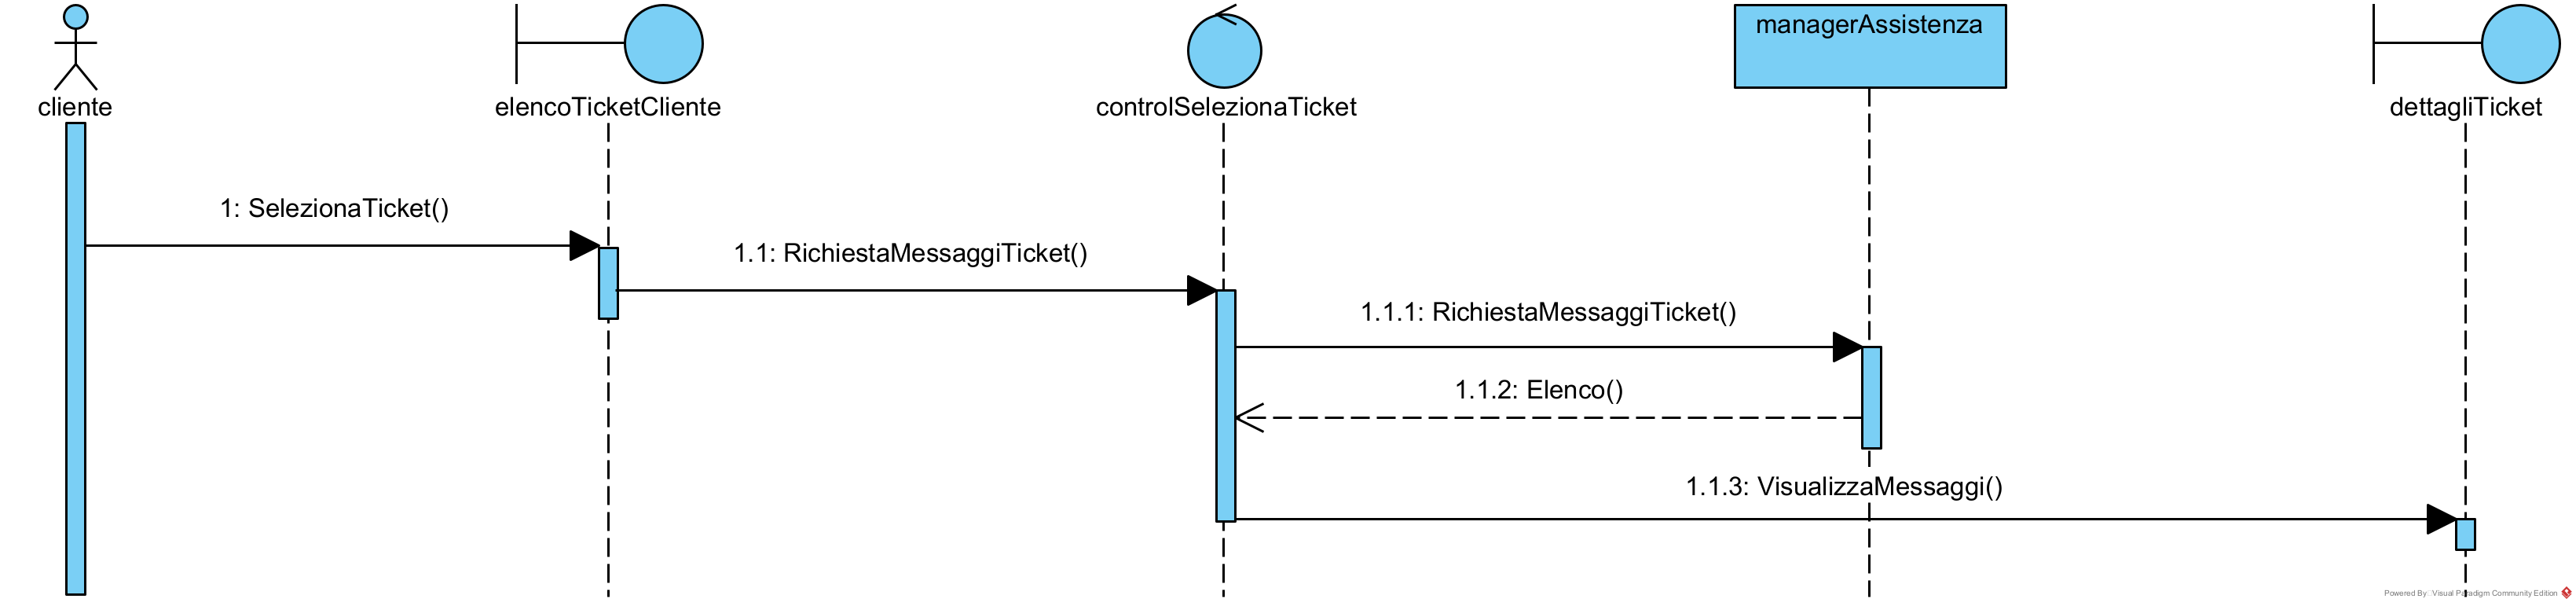
\includegraphics[width=\textwidth]{SequenceDiagram/ClienteTicketSeleziona}
\end{center}

\begin{enumerate}
\item Dall'elenco dei ticket (\ref{SD:elencoticket}), l'utente fa click su uno dei ticket attualmente aperti.
\item Gli vengono mostrati tutti i messaggi inviati fino a quel momento.
\end{enumerate}

\newpage

\subsubsection{Cliente risponde ad un ticket}
\label{SD:rispostaticketcliente}

\begin{center}
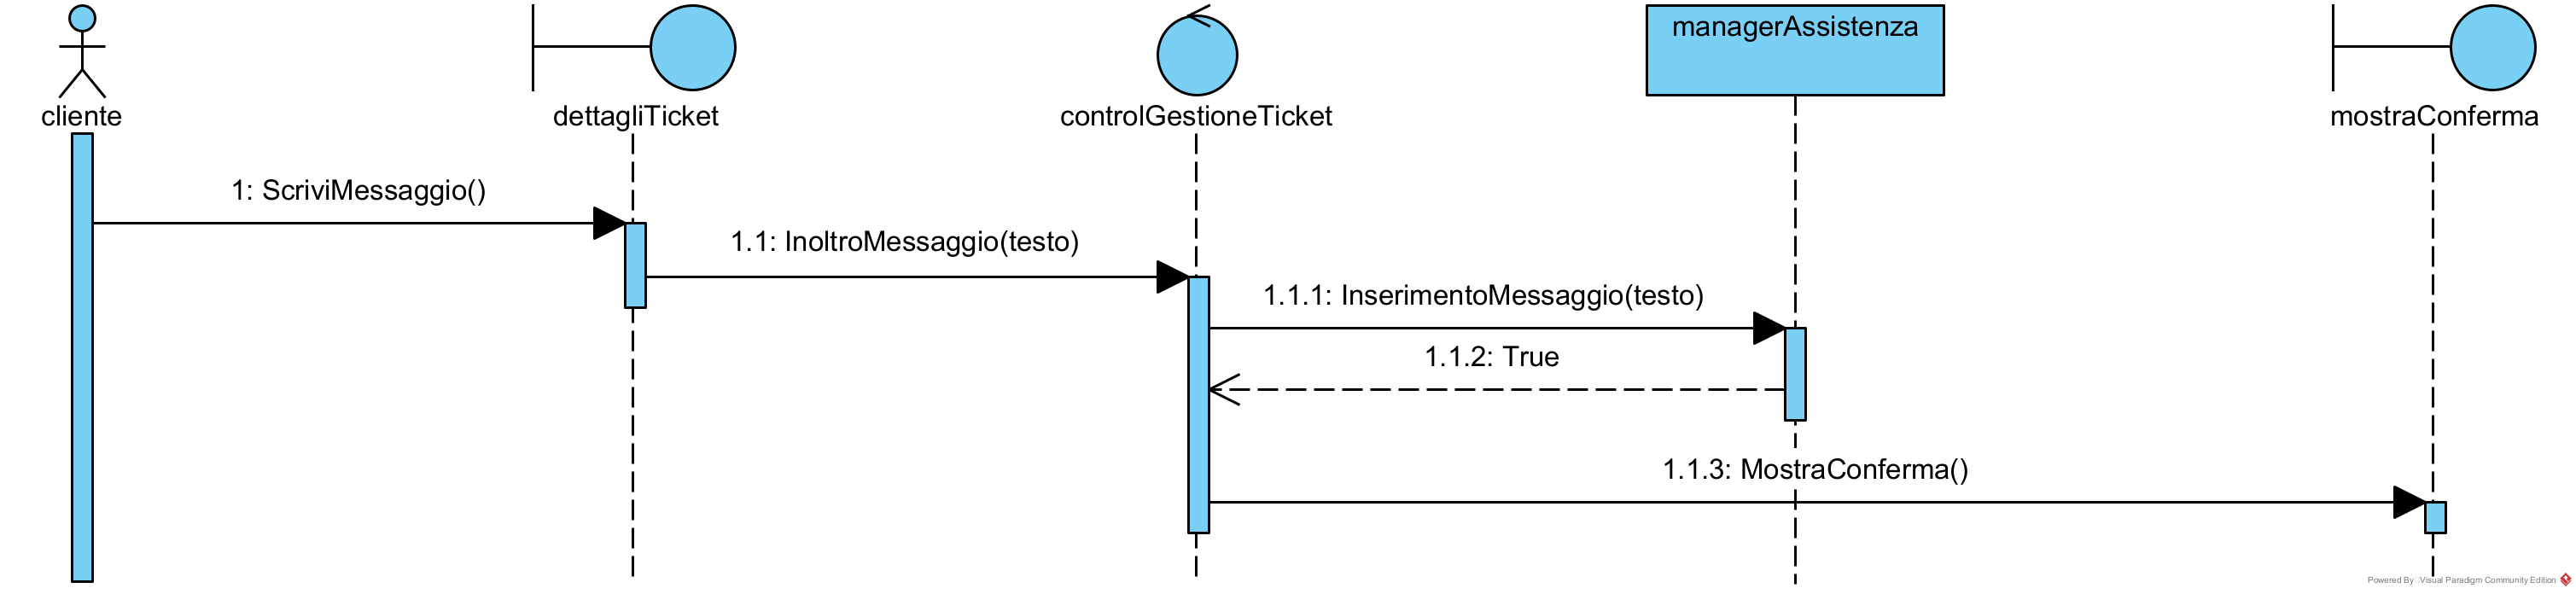
\includegraphics[width=\textwidth]{SequenceDiagram/ClienteTicketRisponde}
\end{center}

\begin{enumerate}
\item Dopo aver selezionato un ticket (\ref{SD:selezioneticketcliente}), l'utente usa il tasto ``Rispondi".
\item Gli viene quindi mostrato un modulo per inserire un nuovo messaggio in risposta al ticket.
\end{enumerate}

\subsubsection{Cliente chiude ticket}
\label{SD:chiusuraticket}

\begin{center}
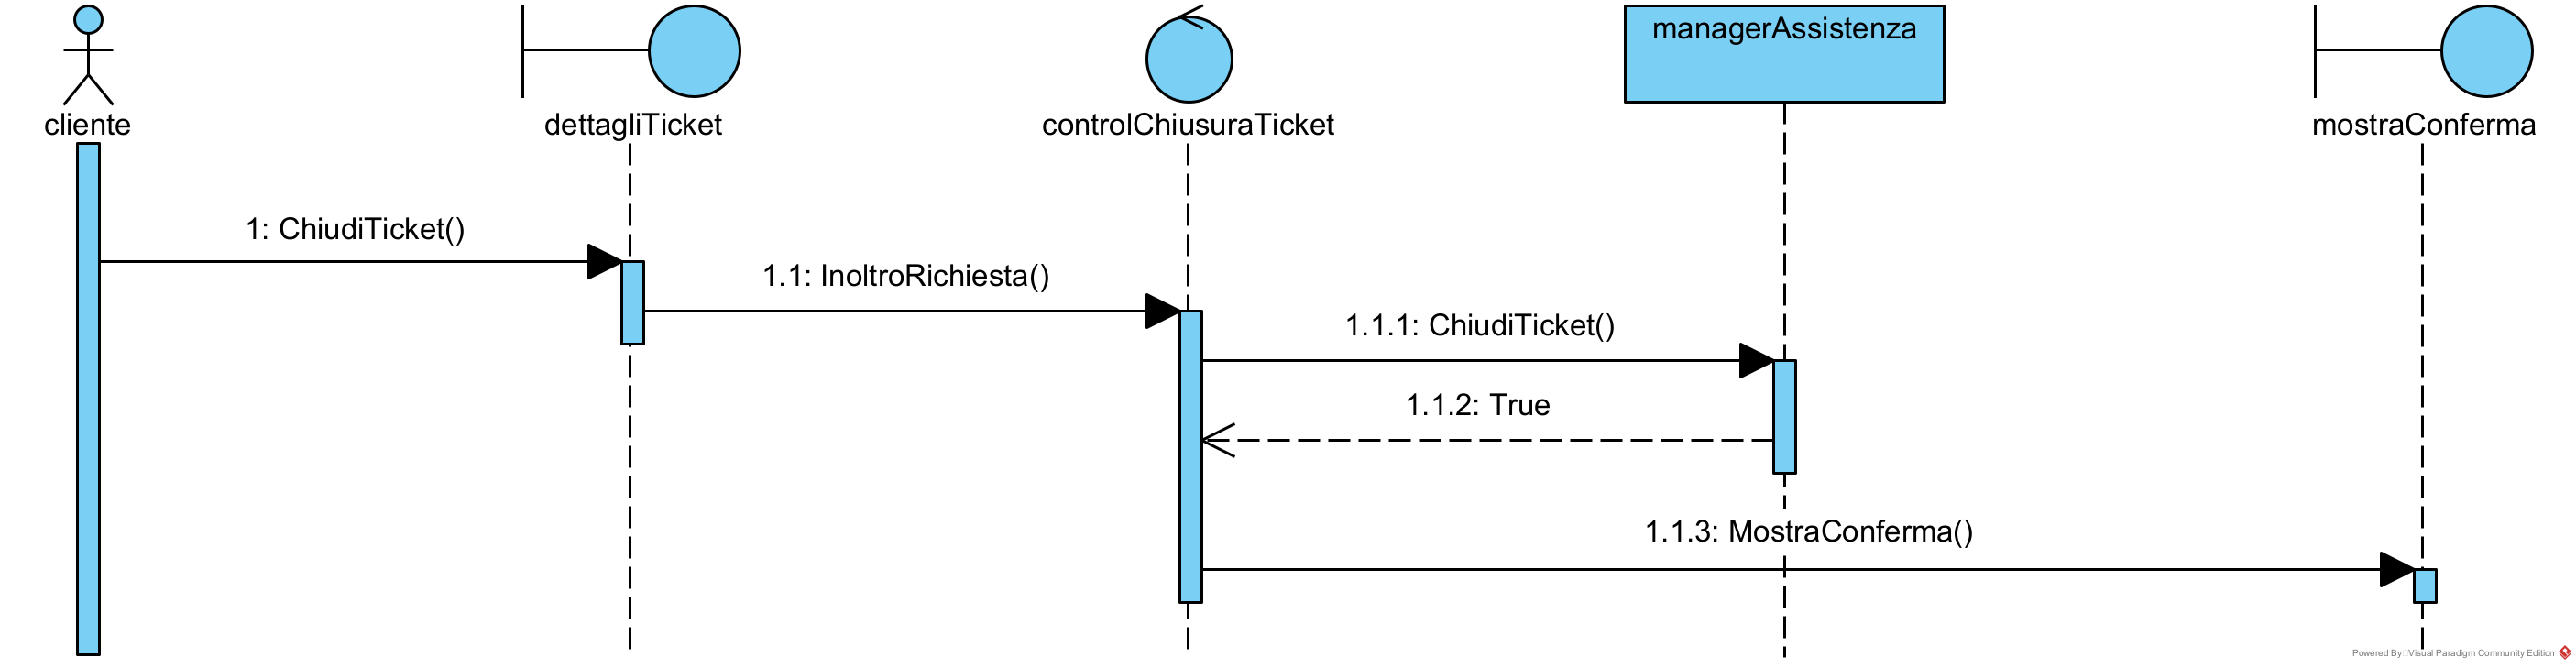
\includegraphics[width=\textwidth]{SequenceDiagram/ClienteTicketChiusura}
\end{center}

\begin{enumerate}
\item Dopo aver selezionato un ticket (\ref{SD:selezioneticketcliente}), l'utente usa il tasto ``Chiudi".
\item Il ticket viene dichiarato chiuso.
\item All'utente viene mostrata una pagina di conferma.
\end{enumerate}

\subsubsection{Cliente recupera password}
\label{SD:recuperopw}

\begin{center}
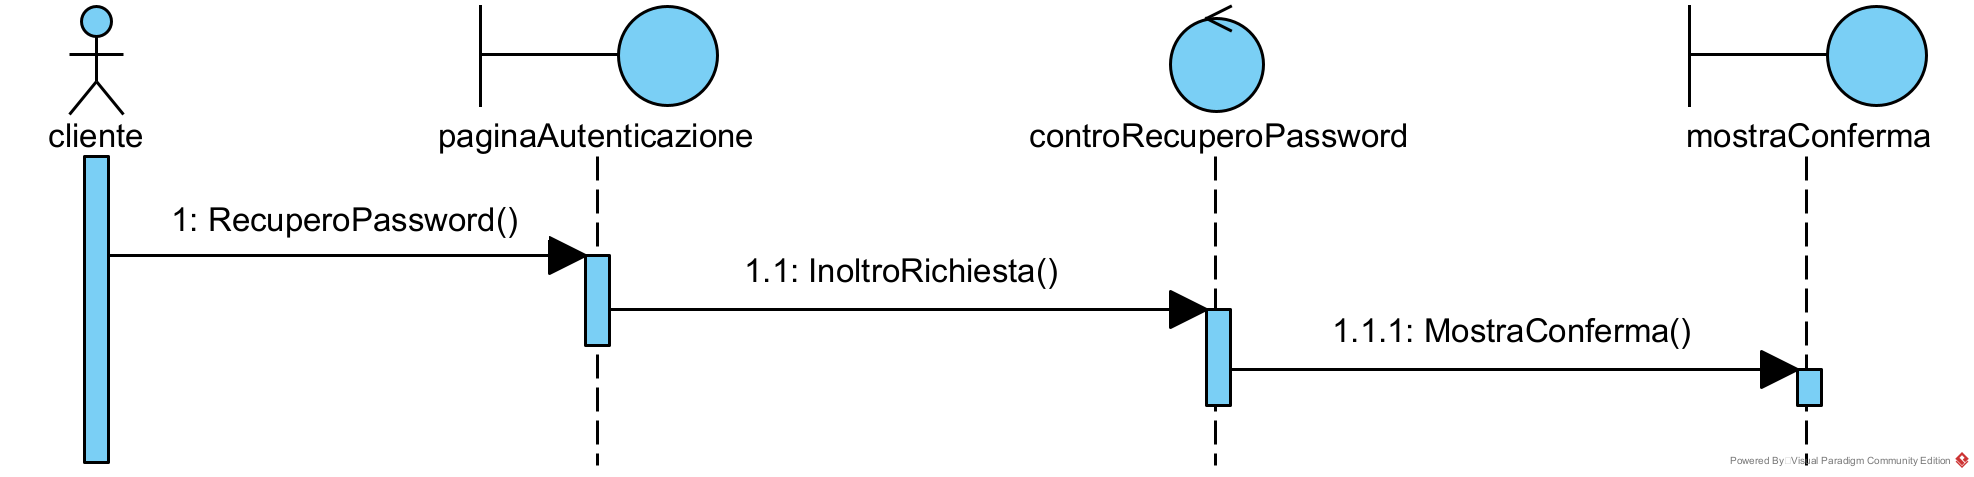
\includegraphics[width=\textwidth]{SequenceDiagram/ClienteRecuperoPassword}
\end{center}

\begin{enumerate}
\item Se un cliente dimentica la sua password, può richiedere di modificarla dalla pagina per l'autenticazione.
\item Il sistema provvede a inviare una mail con un link temporaneo per creare una nuova password.
\end{enumerate}

\subsubsection{Cliente modifica password}
\label{SD:modificapw}

\begin{center}
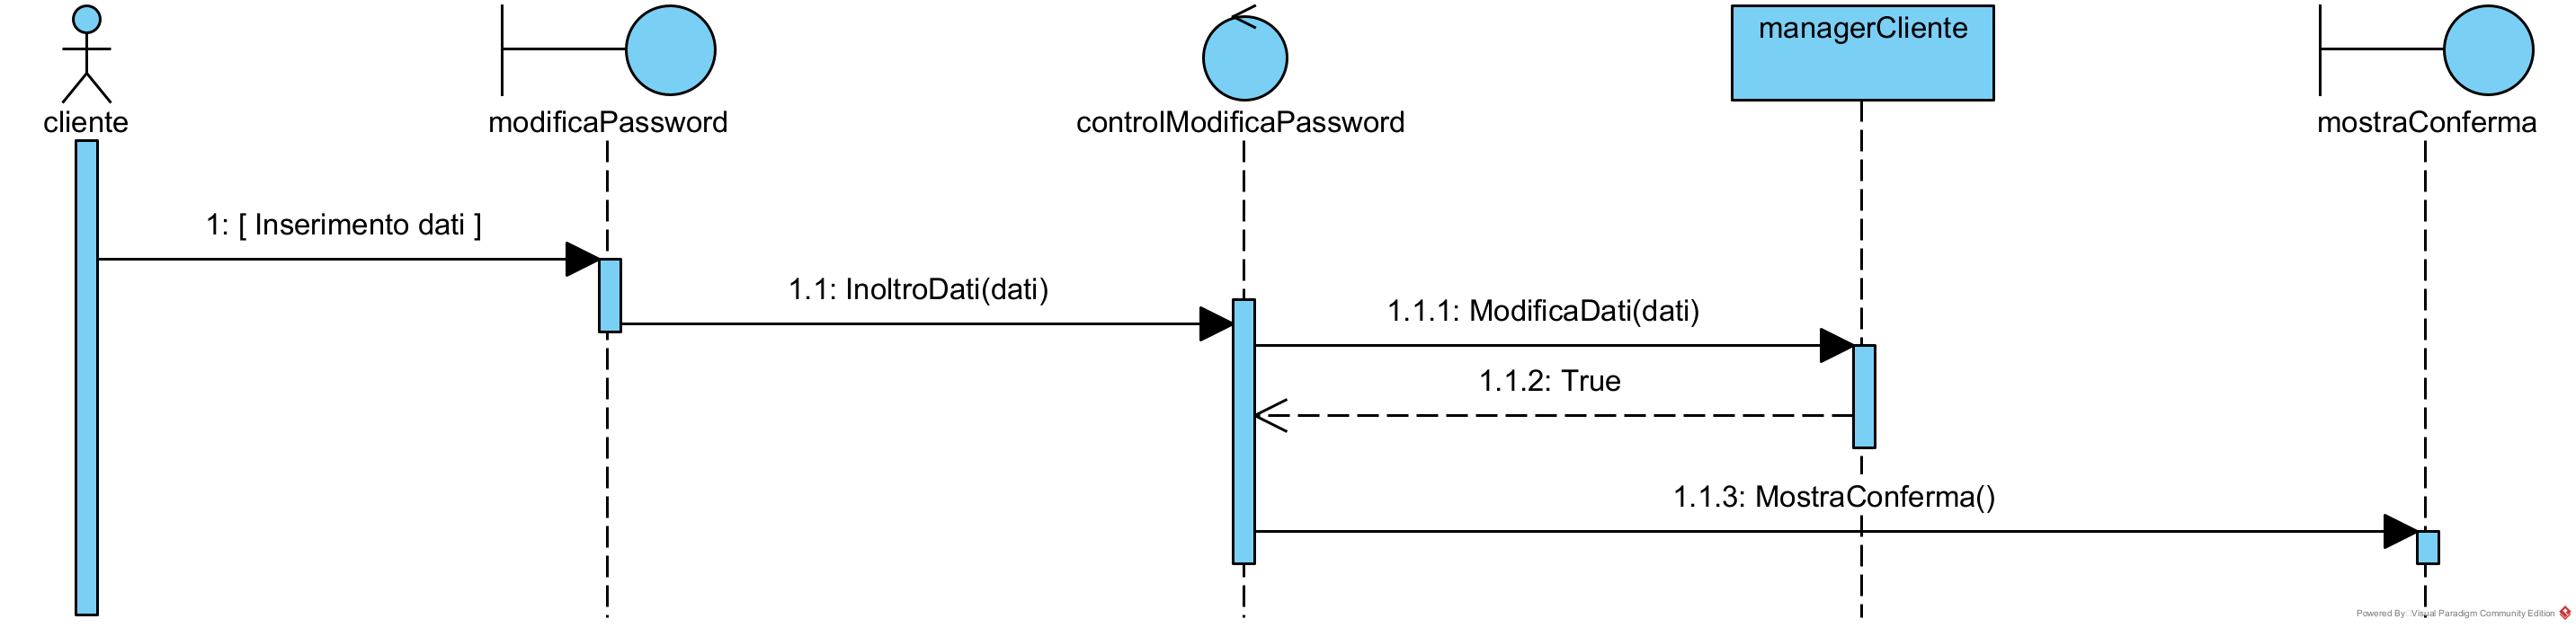
\includegraphics[width=\textwidth]{SequenceDiagram/ClienteModificaPassword}
\end{center}

\begin{enumerate}
\item Se un cliente ha dimenticato la password (\ref{SD:recuperopw}) o se un cliente vuole modificarla per altri motivi, viene rimandato a questo modulo per la modifica.
\item Il sistema provvede a criptare e memorizzare la nuova password per gli accessi futuri.
\end{enumerate}
\newpage

\subsection{Centralinista}

\subsubsection{Centralinista elenca ticket}
\label{SD:centralinistaelencaticket}

\begin{center}
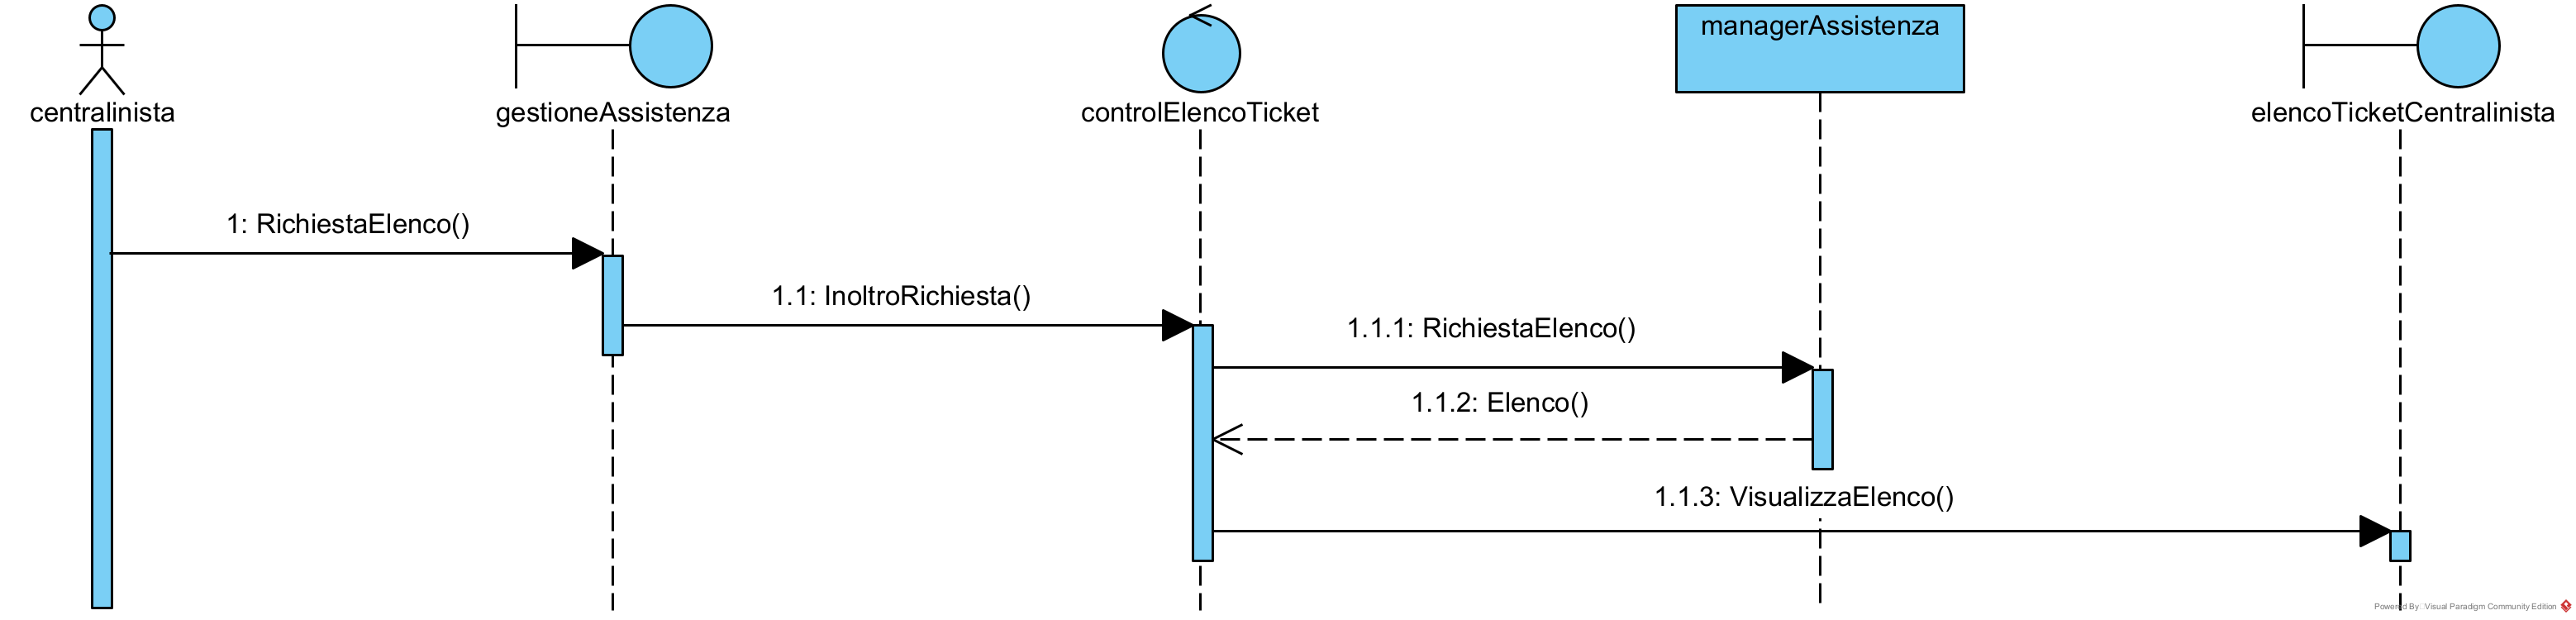
\includegraphics[width=\textwidth]{SequenceDiagram/CentralinistaTicketElenco}
\end{center}

\begin{enumerate}
\item Dopo essersi autenticato (\ref{SD:login}), il centralinista viene rimandato alla pagina iniziale dedicata ai centralinisti. 
\item Da lì può scegliere di visualizzare l'elenco dei ticket in attesa di risposta, ordinati per data crescente.
\end{enumerate}

\subsubsection{Centralinista seleziona un ticket}
\label{SD:selezioneticketcentralinista}

\begin{center}
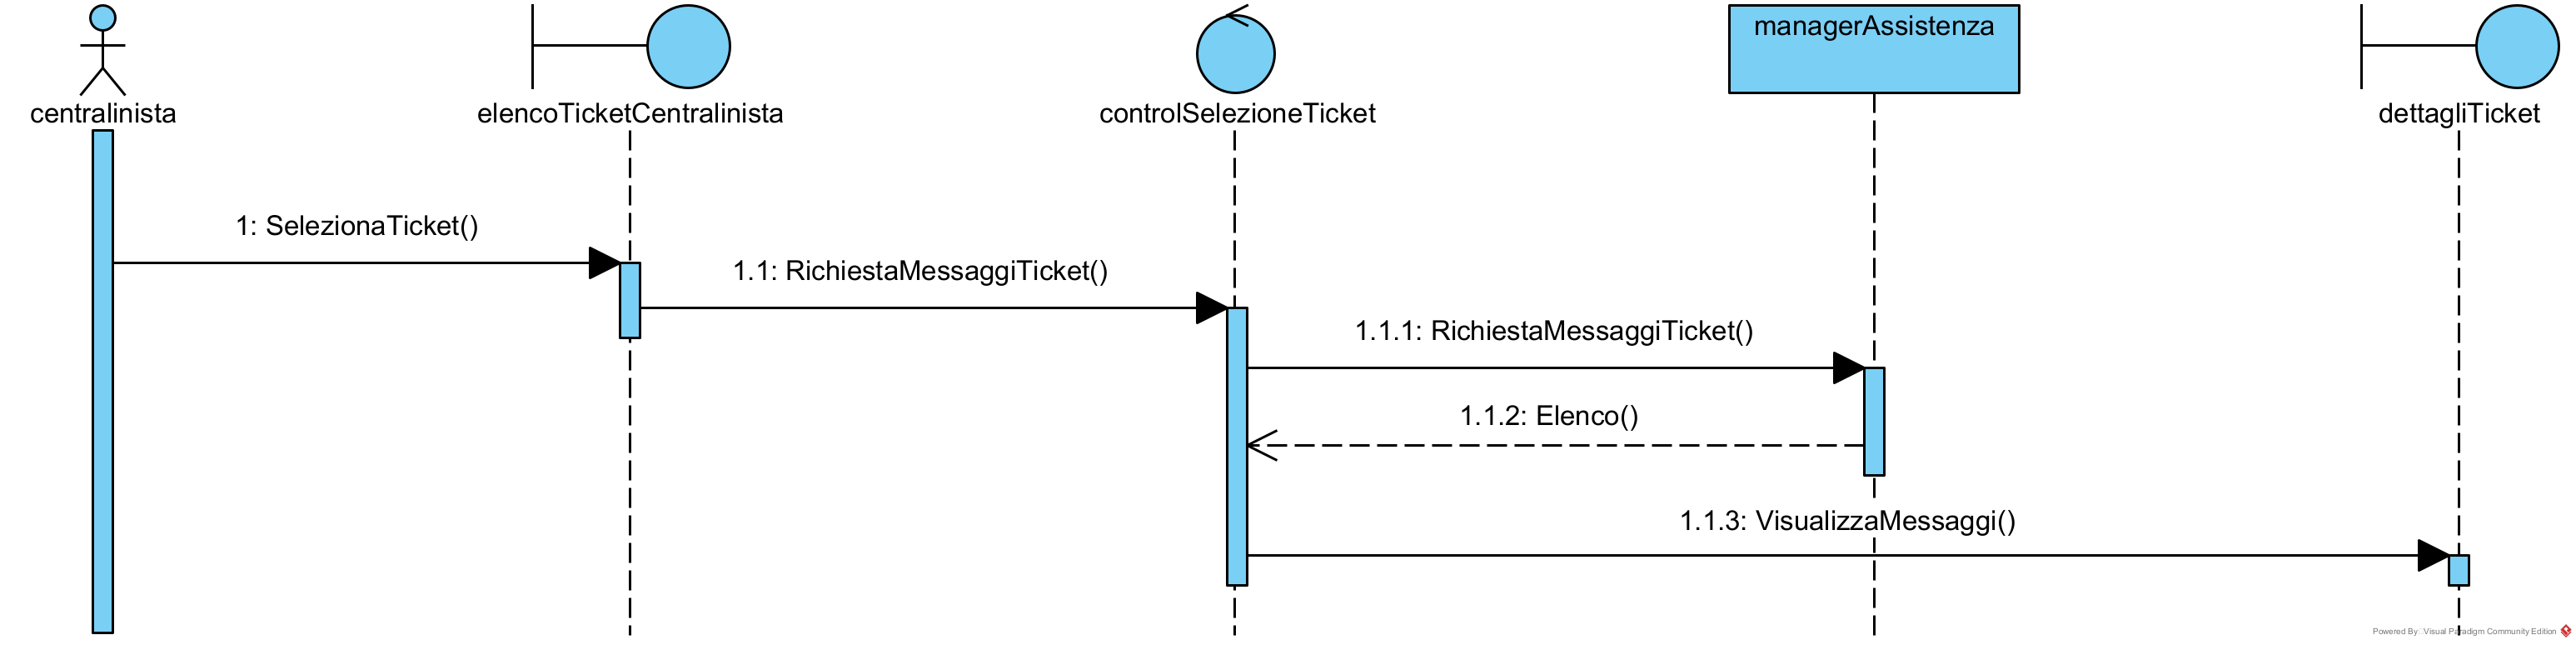
\includegraphics[width=\textwidth]{SequenceDiagram/CentralinistaTicketSeleziona}
\end{center}

\begin{enumerate}
\item Dall'elenco dei ticket (\ref{SD:centralinistaelencaticket}), il centralinista fa click su uno dei ticket attualmente aperti che nello stato di attesa.
\item Lo stato di quel ticket viene cambiato a "In elaborazione".
\item Vengono mostrati tutti i messaggi inviati fino a quel momento.
\end{enumerate}

\newpage

\subsubsection{Centralinista risponde ad un ticket}
\label{SD:rispostaticketcentralinista}

\begin{center}
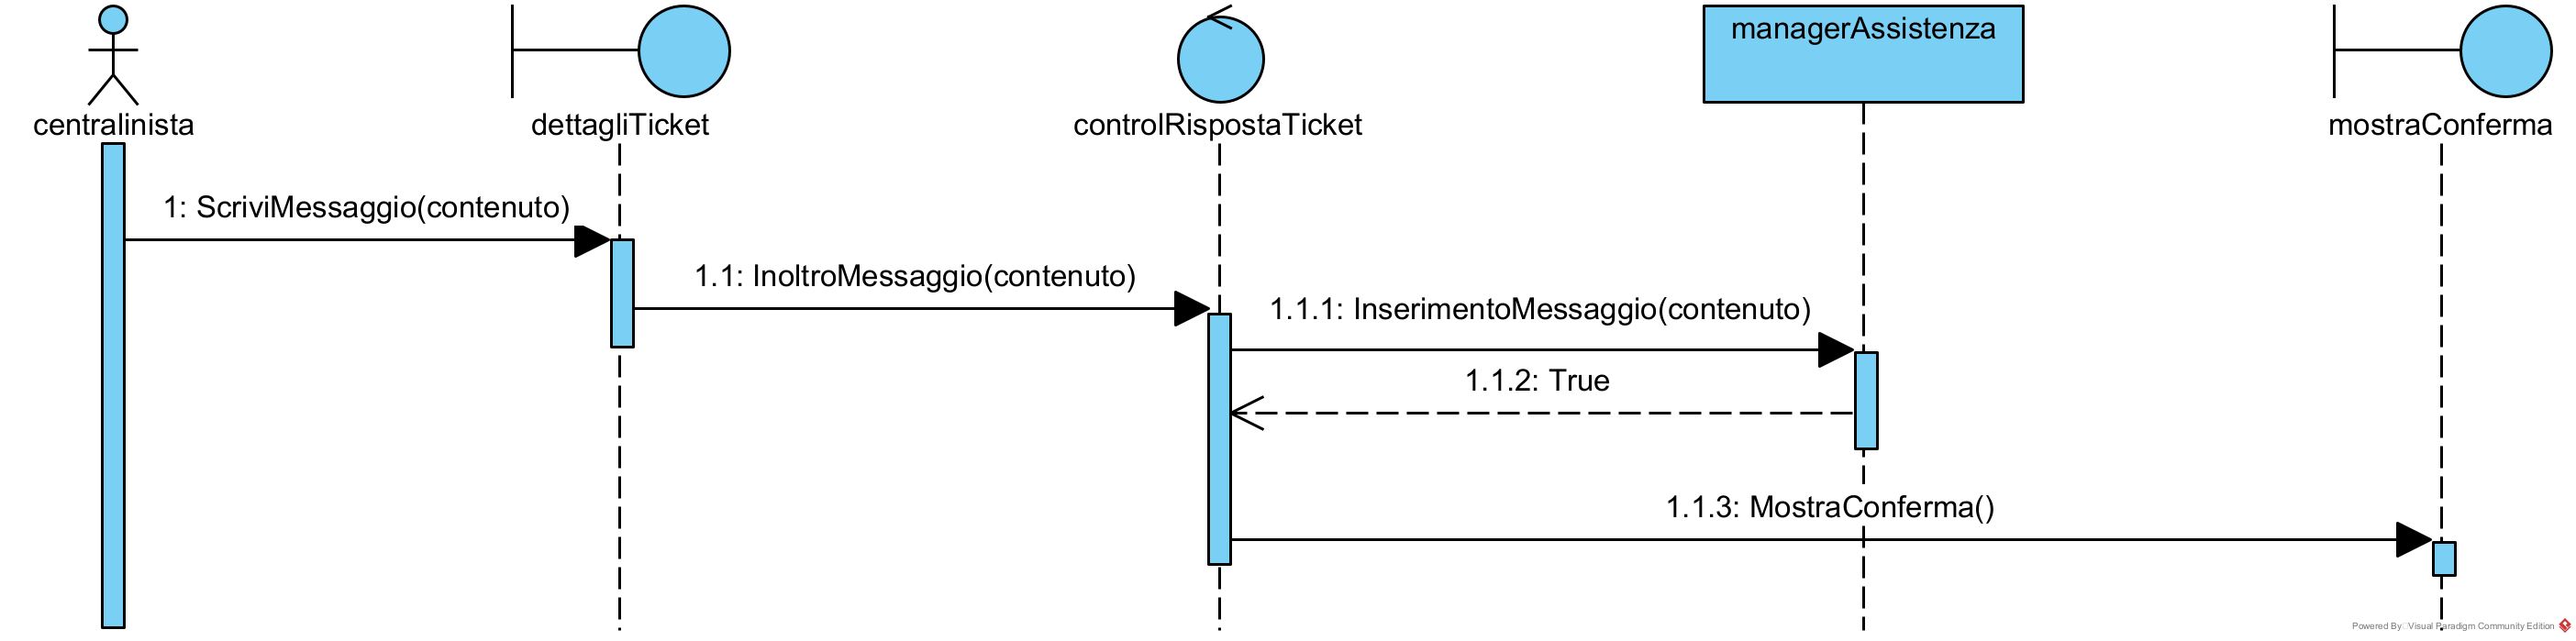
\includegraphics[width=\textwidth]{SequenceDiagram/CentralinistaTicketRisponde}
\end{center}

\begin{enumerate}
\item Dopo aver selezionato un ticket (\ref{SD:selezioneticketcentralinista}), il centralinista usa il tasto ``Rispondi".
\item Gli viene quindi mostrato un modulo per inserire un nuovo messaggio in risposta al ticket.
\item Dopo aver inviato il messaggio, lo stato passa da "In elaborazione" a "In attesa del cliente".
\end{enumerate}

\subsubsection{Centralinista visualizza elenco vendite}
\label{SD:elencovenditecentralinista}

\begin{center}
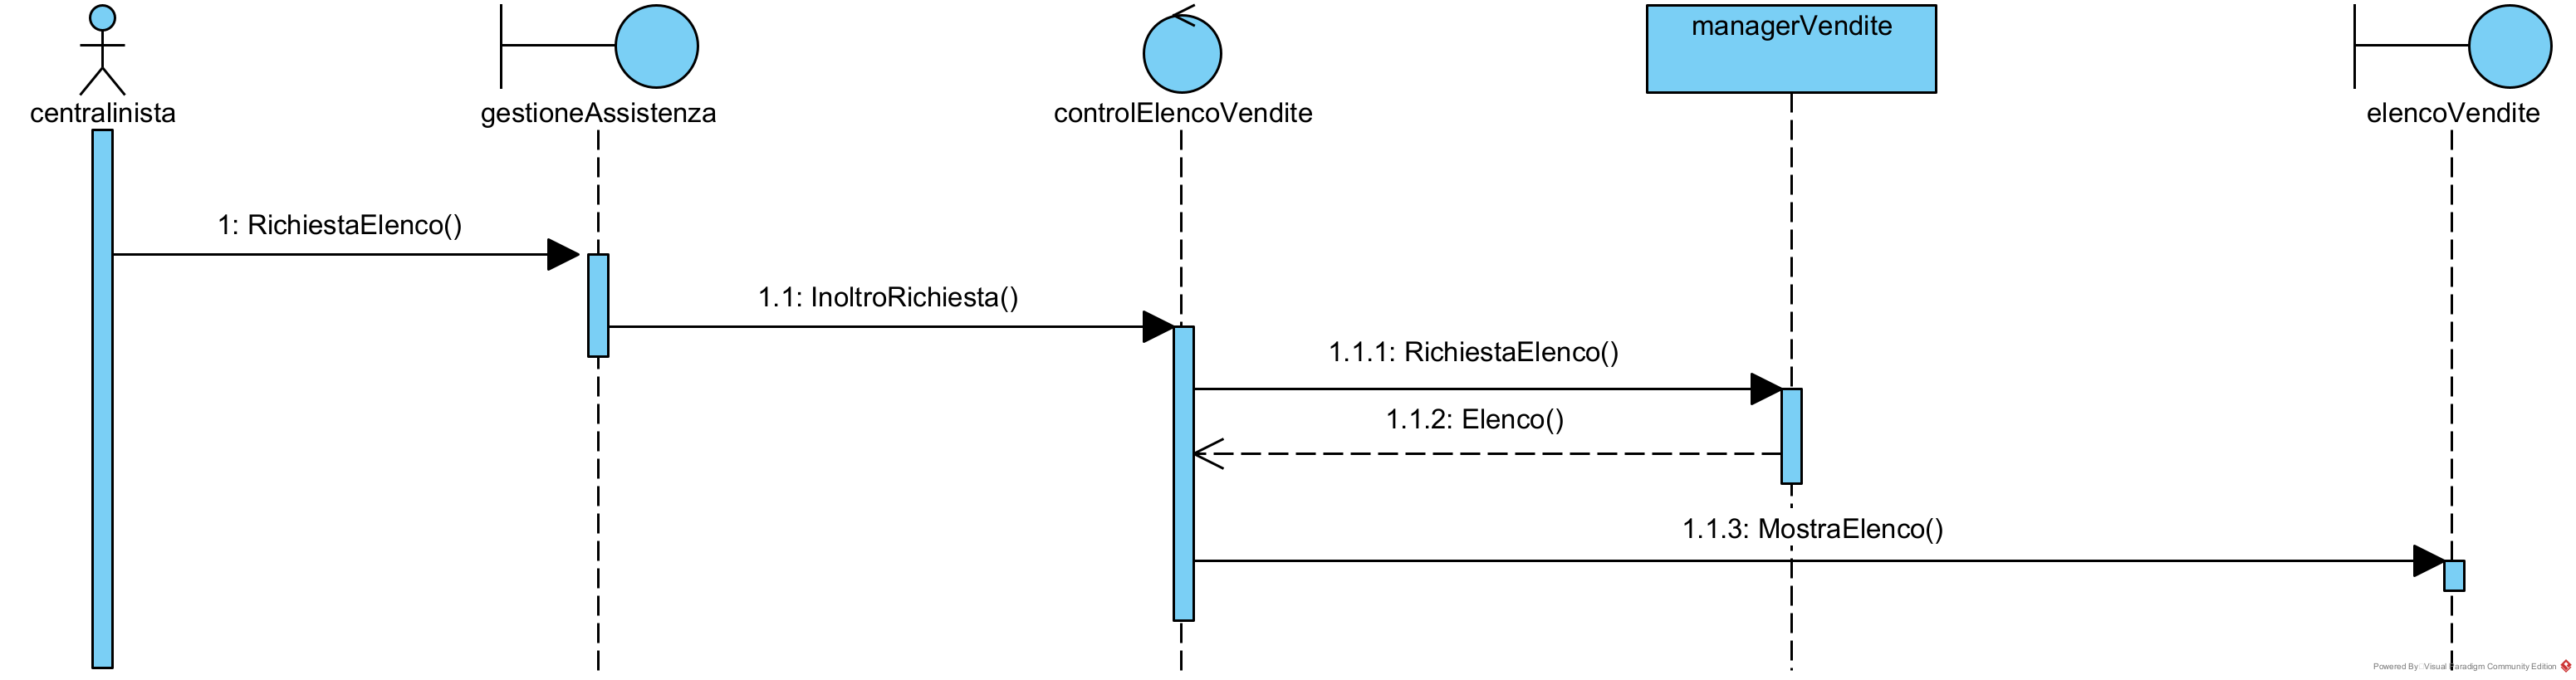
\includegraphics[width=\textwidth]{SequenceDiagram/CentralinistaVenditeElenco}
\end{center}

\begin{enumerate}
\item Dopo essersi autenticato (\ref{SD:login}), il centralinista viene rimandato alla sua homepage. 
\item Da lì potrà scegliere di visualizzare l'elenco delle vendite in attesa di risposta, ordinate per data crescente.
\end{enumerate}

\subsubsection{Centralinista seleziona una vendita}
\label{SD:selezionevenditacentralinista}

\begin{center}
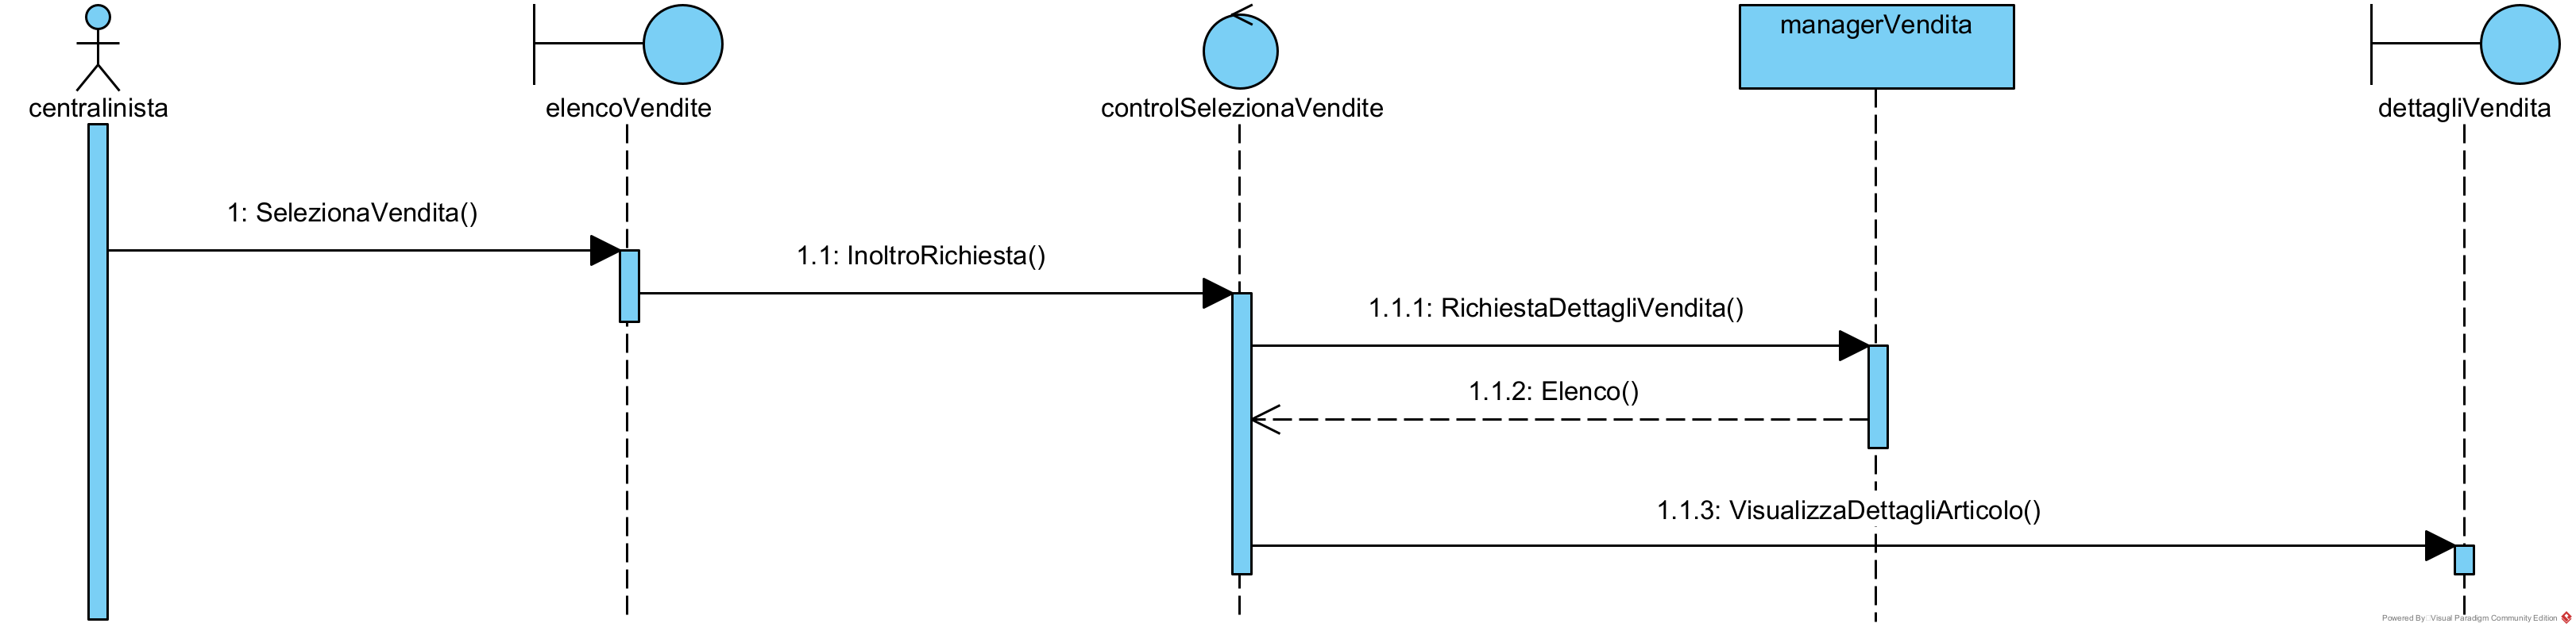
\includegraphics[width=\textwidth]{SequenceDiagram/CentralinistaVenditaSeleziona}
\end{center}

\begin{enumerate}
\item Dall'elenco dei ticket (\ref{SD:centralinistaelencaticket}), il centralinista fa click su una delle vendite attualmente in attesa di conferma.
\item Lo stato della vendita passa a "In elaborazione".
\item Vengono visualizzati tutti i dettagli di quella vendita.
\end{enumerate}

\subsubsection{Centralinista autorizza una vendita}
\label{SD:centralinistaautorizza}
\begin{center}
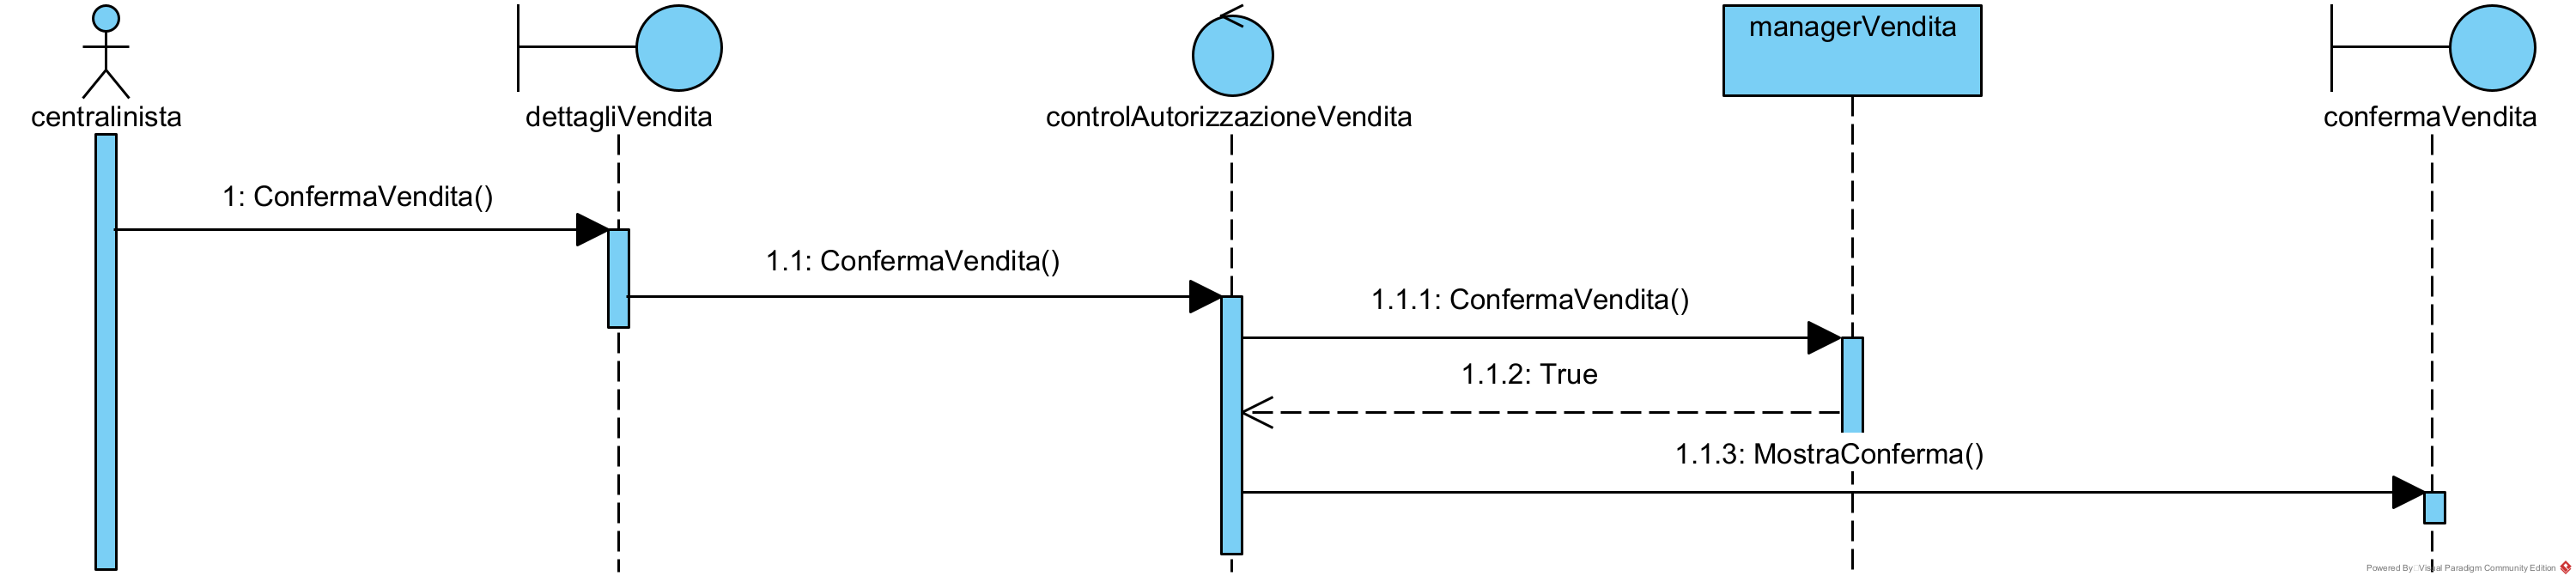
\includegraphics[width=\textwidth]{SequenceDiagram/CentralinistaVenditaAutorizza}
\end{center}

\begin{enumerate}
\item Dopo aver selezionato una vendita (\ref{SD:selezionevenditacentralinista}), il centralinista può autorizzare una vendita.
\end{enumerate}

\subsubsection{Centralinista rifiuta una vendita}
\label{SD:centralinistarifiuta}
\begin{center}
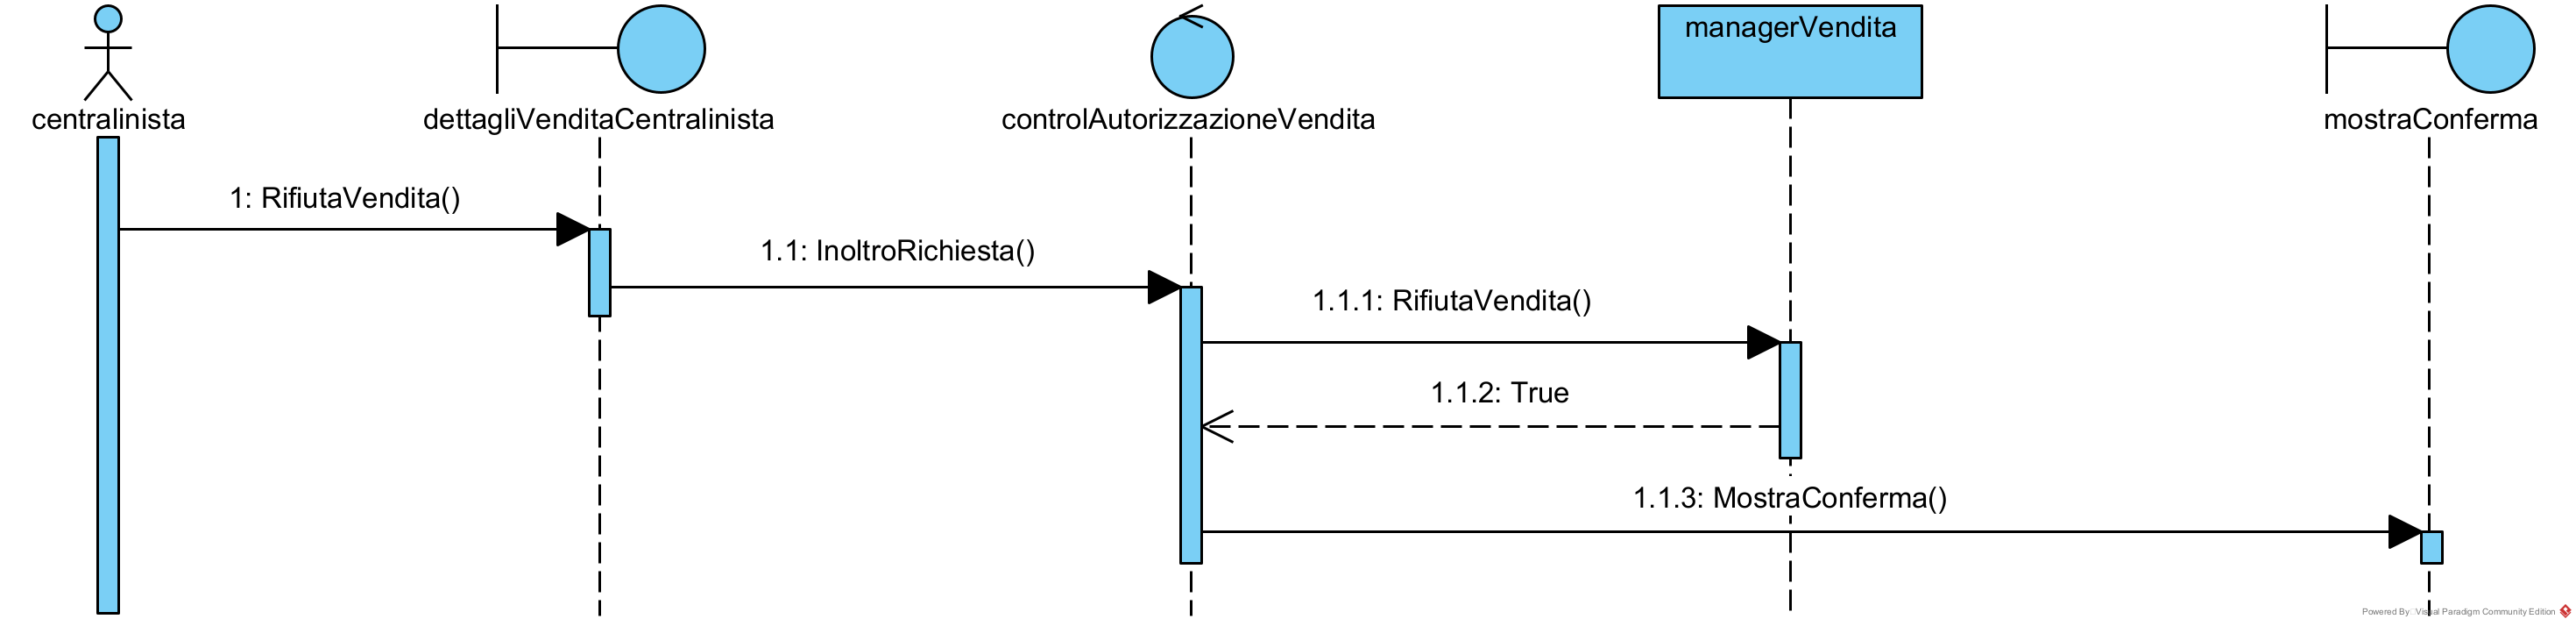
\includegraphics[width=\textwidth]{SequenceDiagram/CentralinistaVenditaRifiuta}
\end{center}

\begin{enumerate}
\item Dopo aver selezionato una vendita (\ref{SD:selezionevenditacentralinista}), il centralinista può rifiutare una vendita.
\end{enumerate}

\newpage

\subsection{Magazziniere}
\subsubsection{Magazziniere elenca ordini}
\label{SD:magazzinierevisualizzaelenco}
\begin{center}
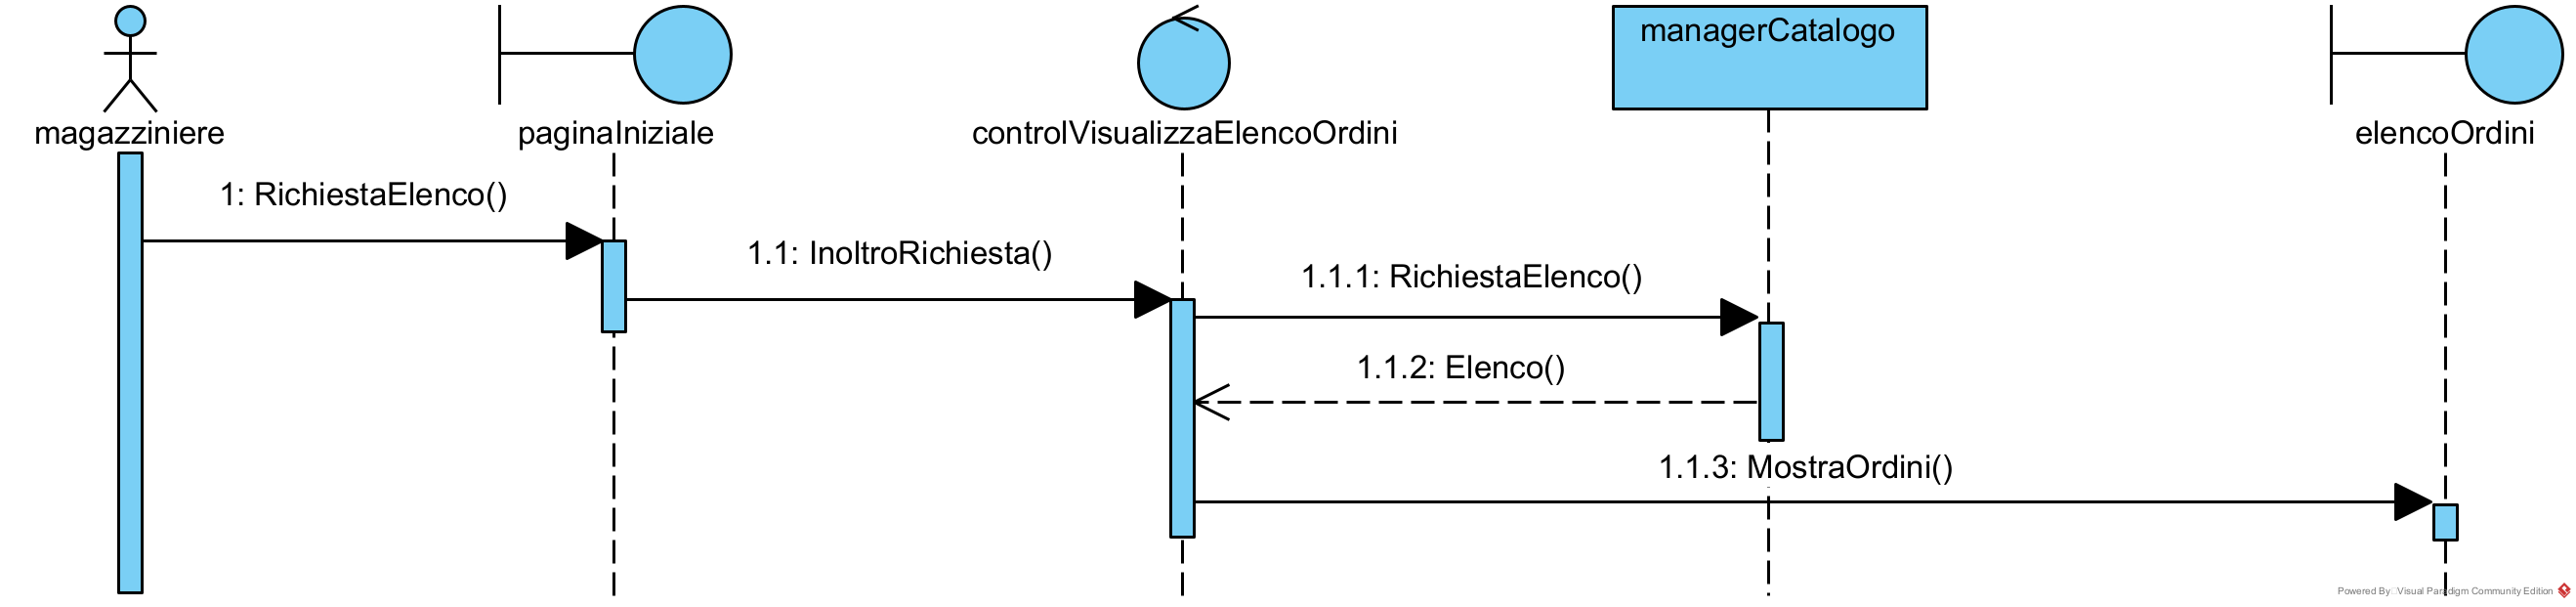
\includegraphics[width=\textwidth]{SequenceDiagram/MagazziniereElencoVisualizza}
\end{center}

\begin{enumerate}
\item Dopo essersi autenticato (\ref{SD:login}), il magazziniere viene rimandato all'elenco degli ordini in attesa di spedizione.
\end{enumerate}

\subsubsection{Magazziniere blocca ordine}
\label{SD:magazziniereblocca}
\begin{center}
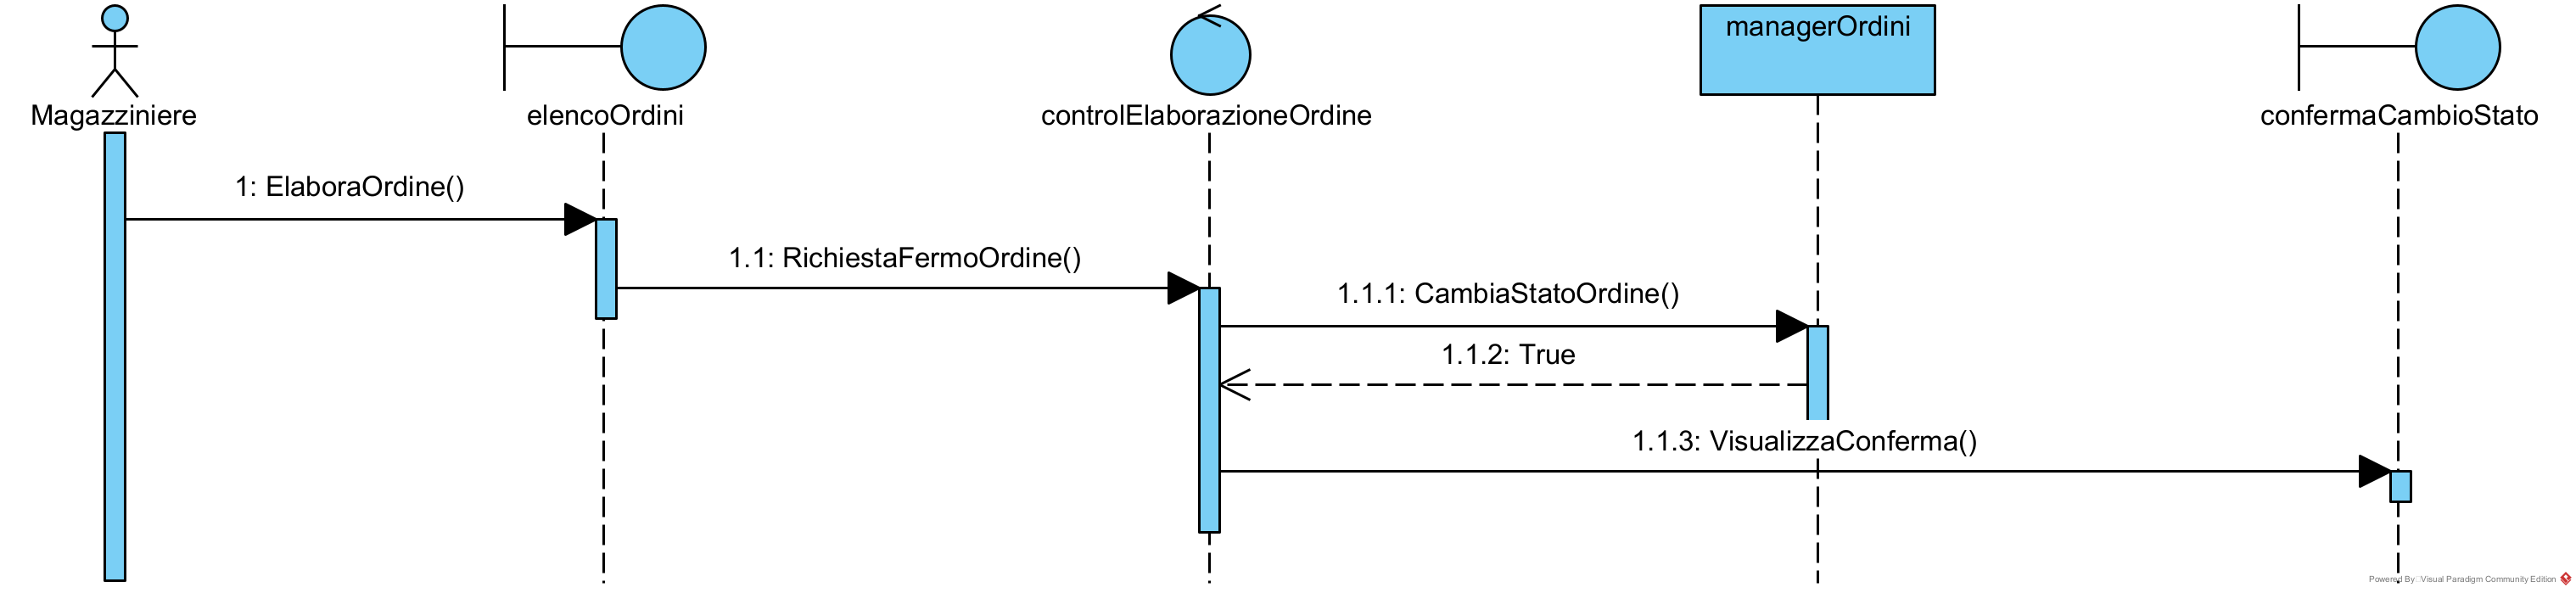
\includegraphics[width=\textwidth]{SequenceDiagram/MagazziniereOrdineBlocca}
\end{center}

\begin{enumerate}
\item Dall'elenco degli ordini (\ref{SD:magazzinierevisualizzaelenco}), il magazziniere può cambiare lo stato di un ordine a ``In elaborazione", in modo che non venga visualizzato dagli altri magazzinieri.
\end{enumerate}

\subsubsection{Magazziniere spedisce ordine}
\label{SD:magazzinierespedisce}
\begin{center}
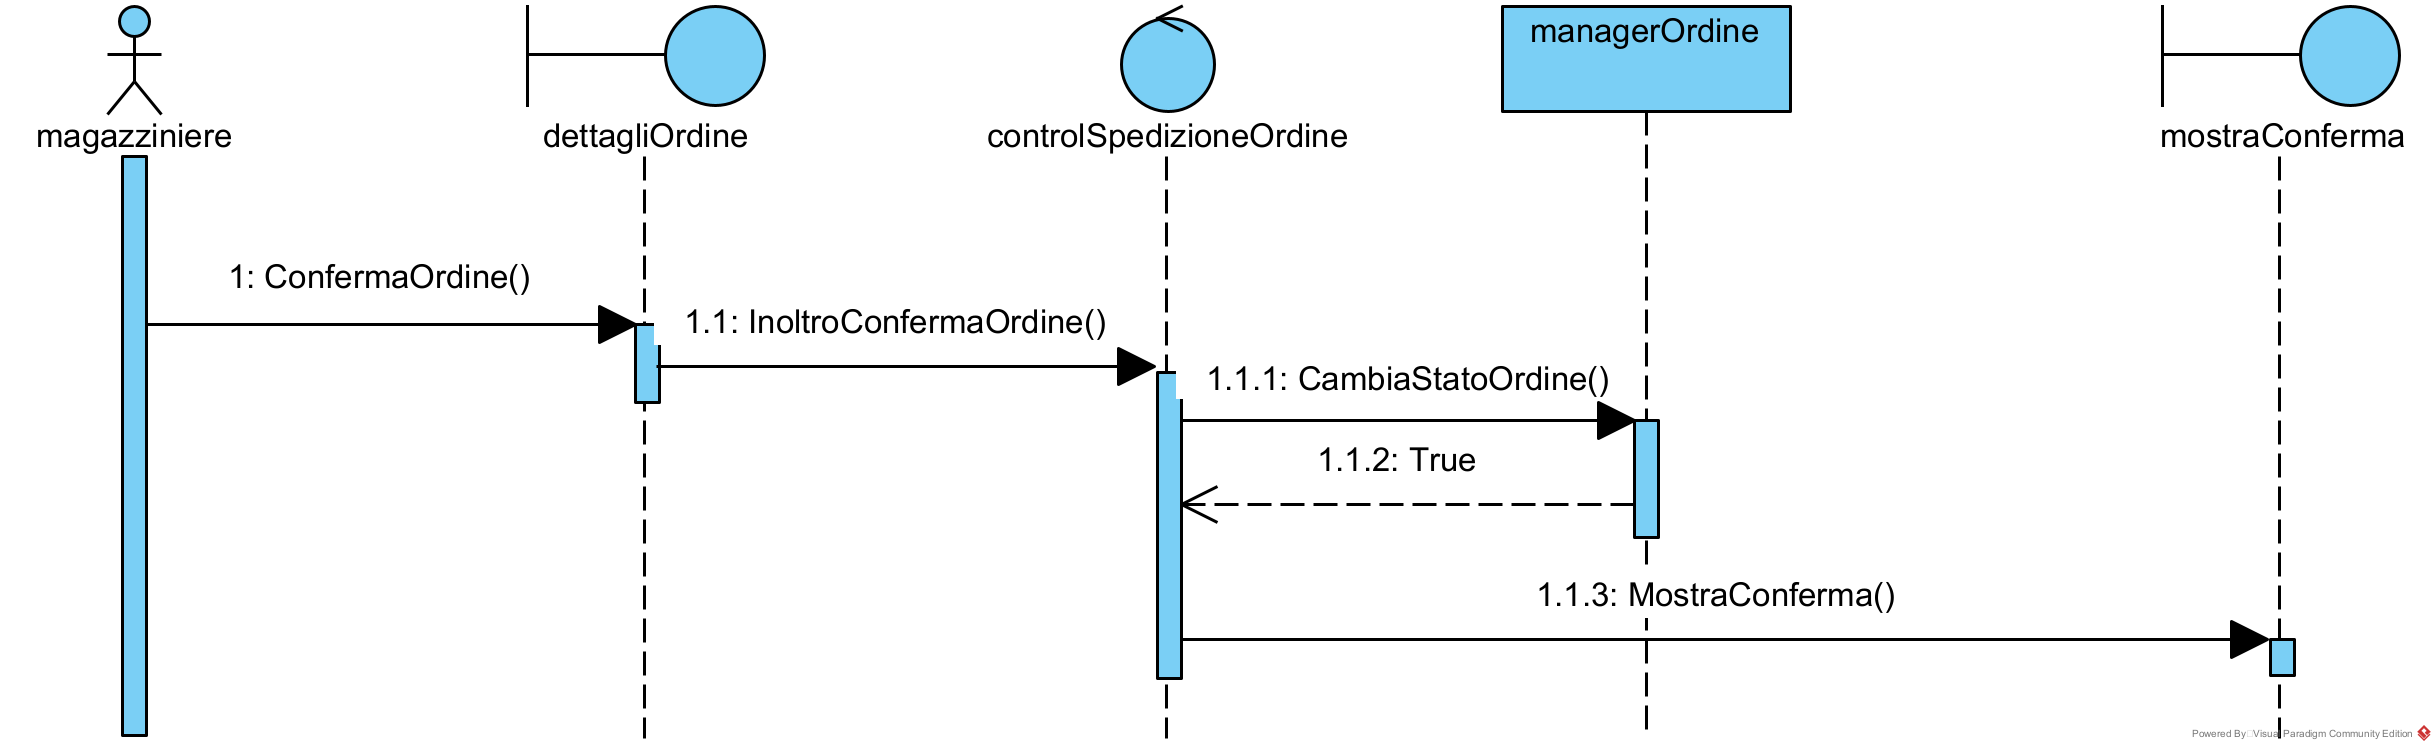
\includegraphics[width=\textwidth]{SequenceDiagram/MagazziniereOrdineSpedisce}
\end{center}

\begin{enumerate}
\item Dall'elenco degli ordini (\ref{SD:magazzinierevisualizzaelenco}), il magazziniere può accettare (\checkmark) un ordine.
\end{enumerate}

\subsubsection{Magazziniere annulla ordine}
\label{SD:magazziniereannulla}
\begin{center}
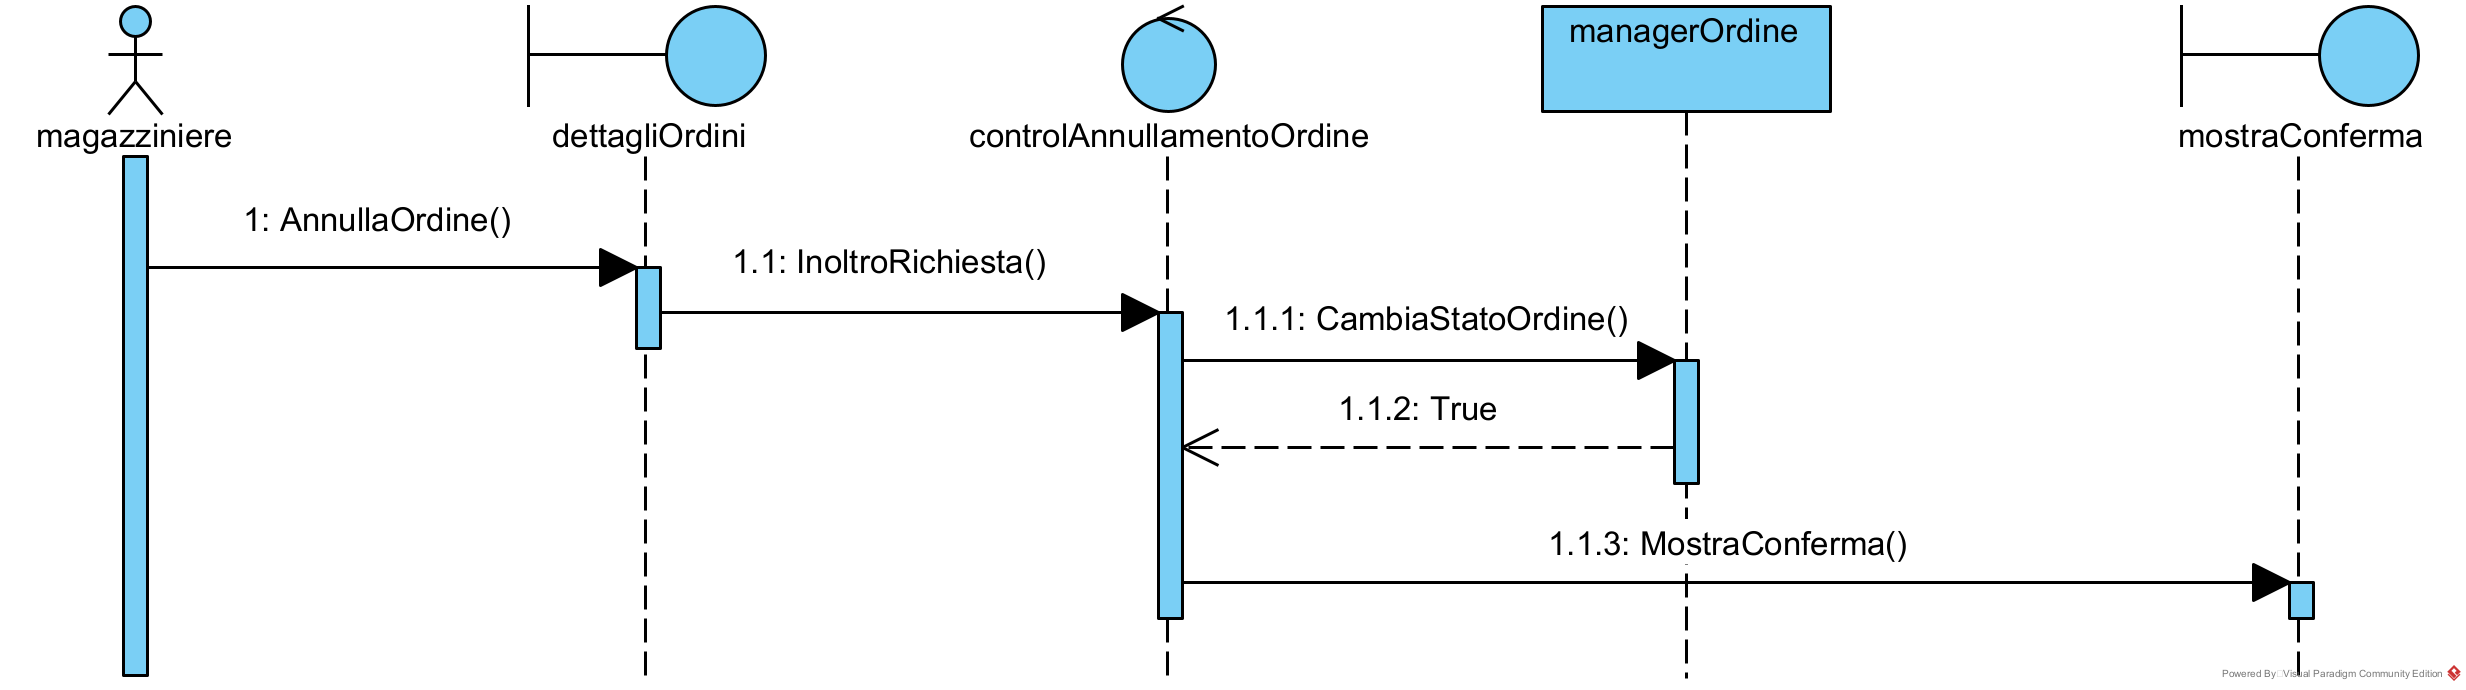
\includegraphics[width=\textwidth]{SequenceDiagram/MagazziniereOrdineAnnulla}
\end{center}

\begin{enumerate}
\item Dall'elenco degli ordini (\ref{SD:magazzinierevisualizzaelenco}), il magazziniere può annullare ($\times$) un ordine.
\end{enumerate}

\newpage

\subsection{Amministratore catalogo}

\subsubsection{Amministratore catalogo ricerca articolo}
\label{SD:amcatvisualizzaelenco}
\begin{center}
\includegraphics[width=\textwidth]{SequenceDiagram/AmministratoreCatalogoVenditaRicerca}
\end{center}

\begin{enumerate}
\item L'amministratore del catalogo può effettuare una ricerca tra gli articoli messi in vendita dalla piattaforma.
\end{enumerate}

\subsubsection{Amministratore catalogo seleziona articolo}
\label{SD:amcatselezionaarticolo}
\begin{center}
\includegraphics[width=\textwidth]{SequenceDiagram/AmministratoreCatalogoVenditaSeleziona}
\end{center}

\begin{enumerate}
\item Dai risultati della ricerca (\ref{SD:amcatvisualizzaelenco}), l'amministratore del catalogo può selezionare uno degli articoli per visualizzarne i dettagli.
\item Viene rimandato a una pagina con i dettagli dell'articolo.
\end{enumerate}

\subsubsection{Amministratore catalogo inserisce articolo}
\label{SD:amcatinseriscearticolo}
\begin{center}
\includegraphics[width=\textwidth]{SequenceDiagram/AmministratoreCatalogoVenditaCrea}
\end{center}

\begin{enumerate}
\item Dall'elenco (\ref{SD:amcatvisualizzaelenco}), l'amministratore del catalogo può inserire un nuovo articolo usando il tasto ``Nuovo articolo".
\item Viene rimandato ad un modulo per l'inserimento dei dati necessari come nome, prezzo, quantità disponibile e foto.
\item L'articolo viene immediatamente messo in vendita.
\end{enumerate}

\subsubsection{Amministratore catalogo modifica articolo}
\label{SD:amcatmodificaarticolo}
\begin{center}
\includegraphics[width=\textwidth]{SequenceDiagram/AmministratoreCatalogoVenditaModifica}
\end{center}

\begin{enumerate}
\item Dai risultati della ricerca (\ref{SD:amcatvisualizzaelenco}), l'amministratore del catalogo può modificare i dettagli di un articolo.
\item Cliccando il tasto ``Modifica" visualizzerà una pagina con un modulo per la modifica delle informazioni.
\end{enumerate}

\subsubsection{Amministratore catalogo rimuove articolo}
\label{SD:amcatrimuovearticolo}
\begin{center}
\includegraphics[width=\textwidth]{SequenceDiagram/AmministratoreCatalogoVenditaRimuove}
\end{center}

\begin{enumerate}
\item Dai risultati della ricerca (\ref{SD:amcatvisualizzaelenco}), l'amministratore del catalogo può rimuovere un articolo usando il tasto ``Rimuovi".
\end{enumerate}

\newpage

\subsection{Amministratore personale}
\subsubsection{Amministratore personale ricerca dipendente}
\label{SD:amperricerca}
\begin{center}
\includegraphics[width=\textwidth]{SequenceDiagram/AmministratorePersonaleDipendenteRicerca}
\end{center}

\begin{enumerate}
\item L'amministratore del personale può effettuare una ricerca tra i dipendenti.
\end{enumerate}

\subsubsection{Amministratore personale seleziona dipendente}
\label{SD:amperselezione}
\begin{center}
\includegraphics[width=\textwidth]{SequenceDiagram/AmministratorePersonaleDipendenteSeleziona}
\end{center}

\begin{enumerate}
\item Dall'elenco (\ref{SD:amcatvisualizzaelenco}), l'amministratore del personale potrà selezionare uno dei dipendenti per visualizzarne i dettagli e le statistiche come il numero di ordini spediti o il numero di ticket a cui hanno risposto, in base alla tipologia di dipendente.
\end{enumerate}

\subsubsection{Amministratore personale inserisce dipendente}
\label{SD:amperinserisce}
\begin{center}
\includegraphics[width=\textwidth]{SequenceDiagram/AmministratorePersonaleDipendenteInserisce}
\end{center}

\begin{enumerate}
\item Dall'elenco (\ref{SD:amcatvisualizzaelenco}), l'amministratore del personale può inserire un nuovo dipendente.
\item Viene rimandato ad un modulo per l'inserimento dei dati richiesti come nome, cognome, indirizzo e ruolo.
\end{enumerate}

\subsubsection{Amministratore personale modifica dipendente}
\label{SD:ampermodifica}
\begin{center}
\includegraphics[width=\textwidth]{SequenceDiagram/AmministratorePersonaleDipendenteModifica}
\end{center}

\begin{enumerate}
\item Dalla pagina dei dettagli di un dipendente (\ref{SD:amperselezione}), l'amministratore del personale può modificare i dettagli di un dipendente usando il tasto ``Modifica".
\item Visualizza una pagina con un modulo per la modifica delle informazioni.
\end{enumerate}

\subsubsection{Amministratore personale rimuove dipendente}
\label{SD:amperrimuove}
\begin{center}
\includegraphics[width=\textwidth]{SequenceDiagram/AmministratorePersonaleDipendenteRimuove}
\end{center}


\begin{enumerate}
\item Dalla pagina dei dettagli di un articolo (\ref{SD:amcatselezionaarticolo}), l'amministratore del catalogo può rimuovere un articolo usando il tasto ``Rimuovi".
\item Visualizza una pagina di conferma.
\end{enumerate}

\newpage

\section{Statechart Diagram}

\subsection{Ordine}
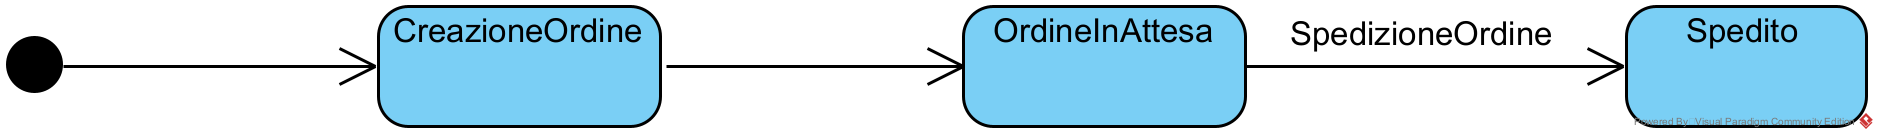
\includegraphics[width=\textwidth]{StateChart/Ordine}

\subsection{Ticket}
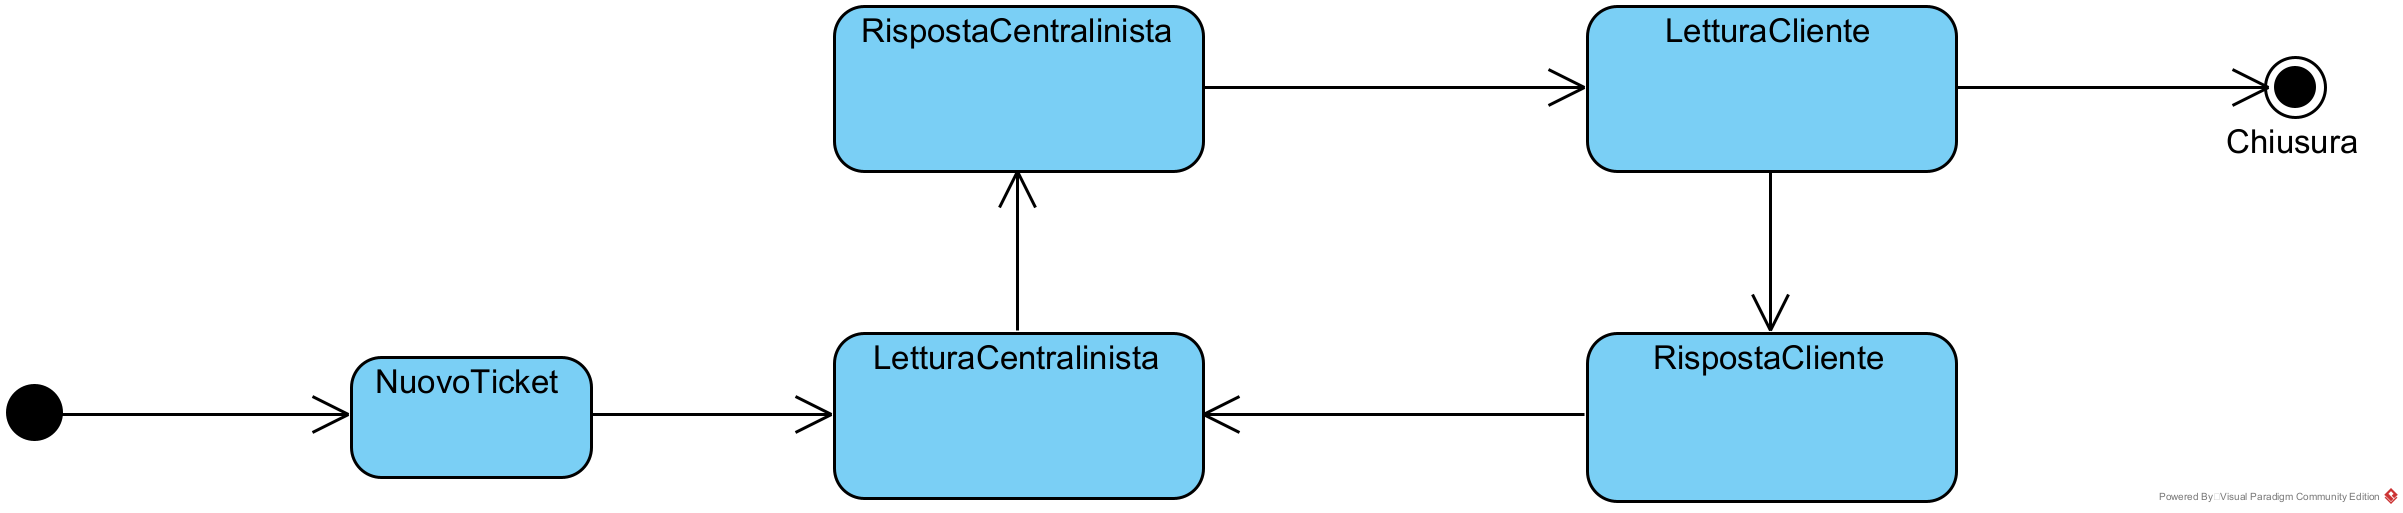
\includegraphics[width=\textwidth]{StateChart/Ticket}

\subsection{Vendita}
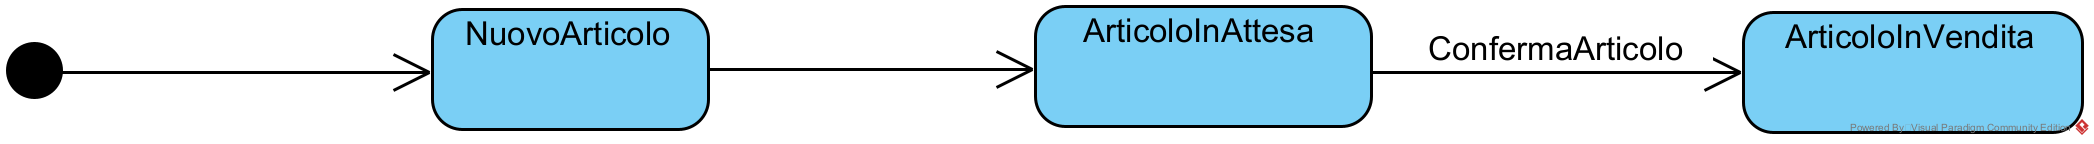
\includegraphics[width=\textwidth]{StateChart/Vendita}

\newpage

\section{Activity Diagram}

\subsection{Registrazione}
\begin{center}
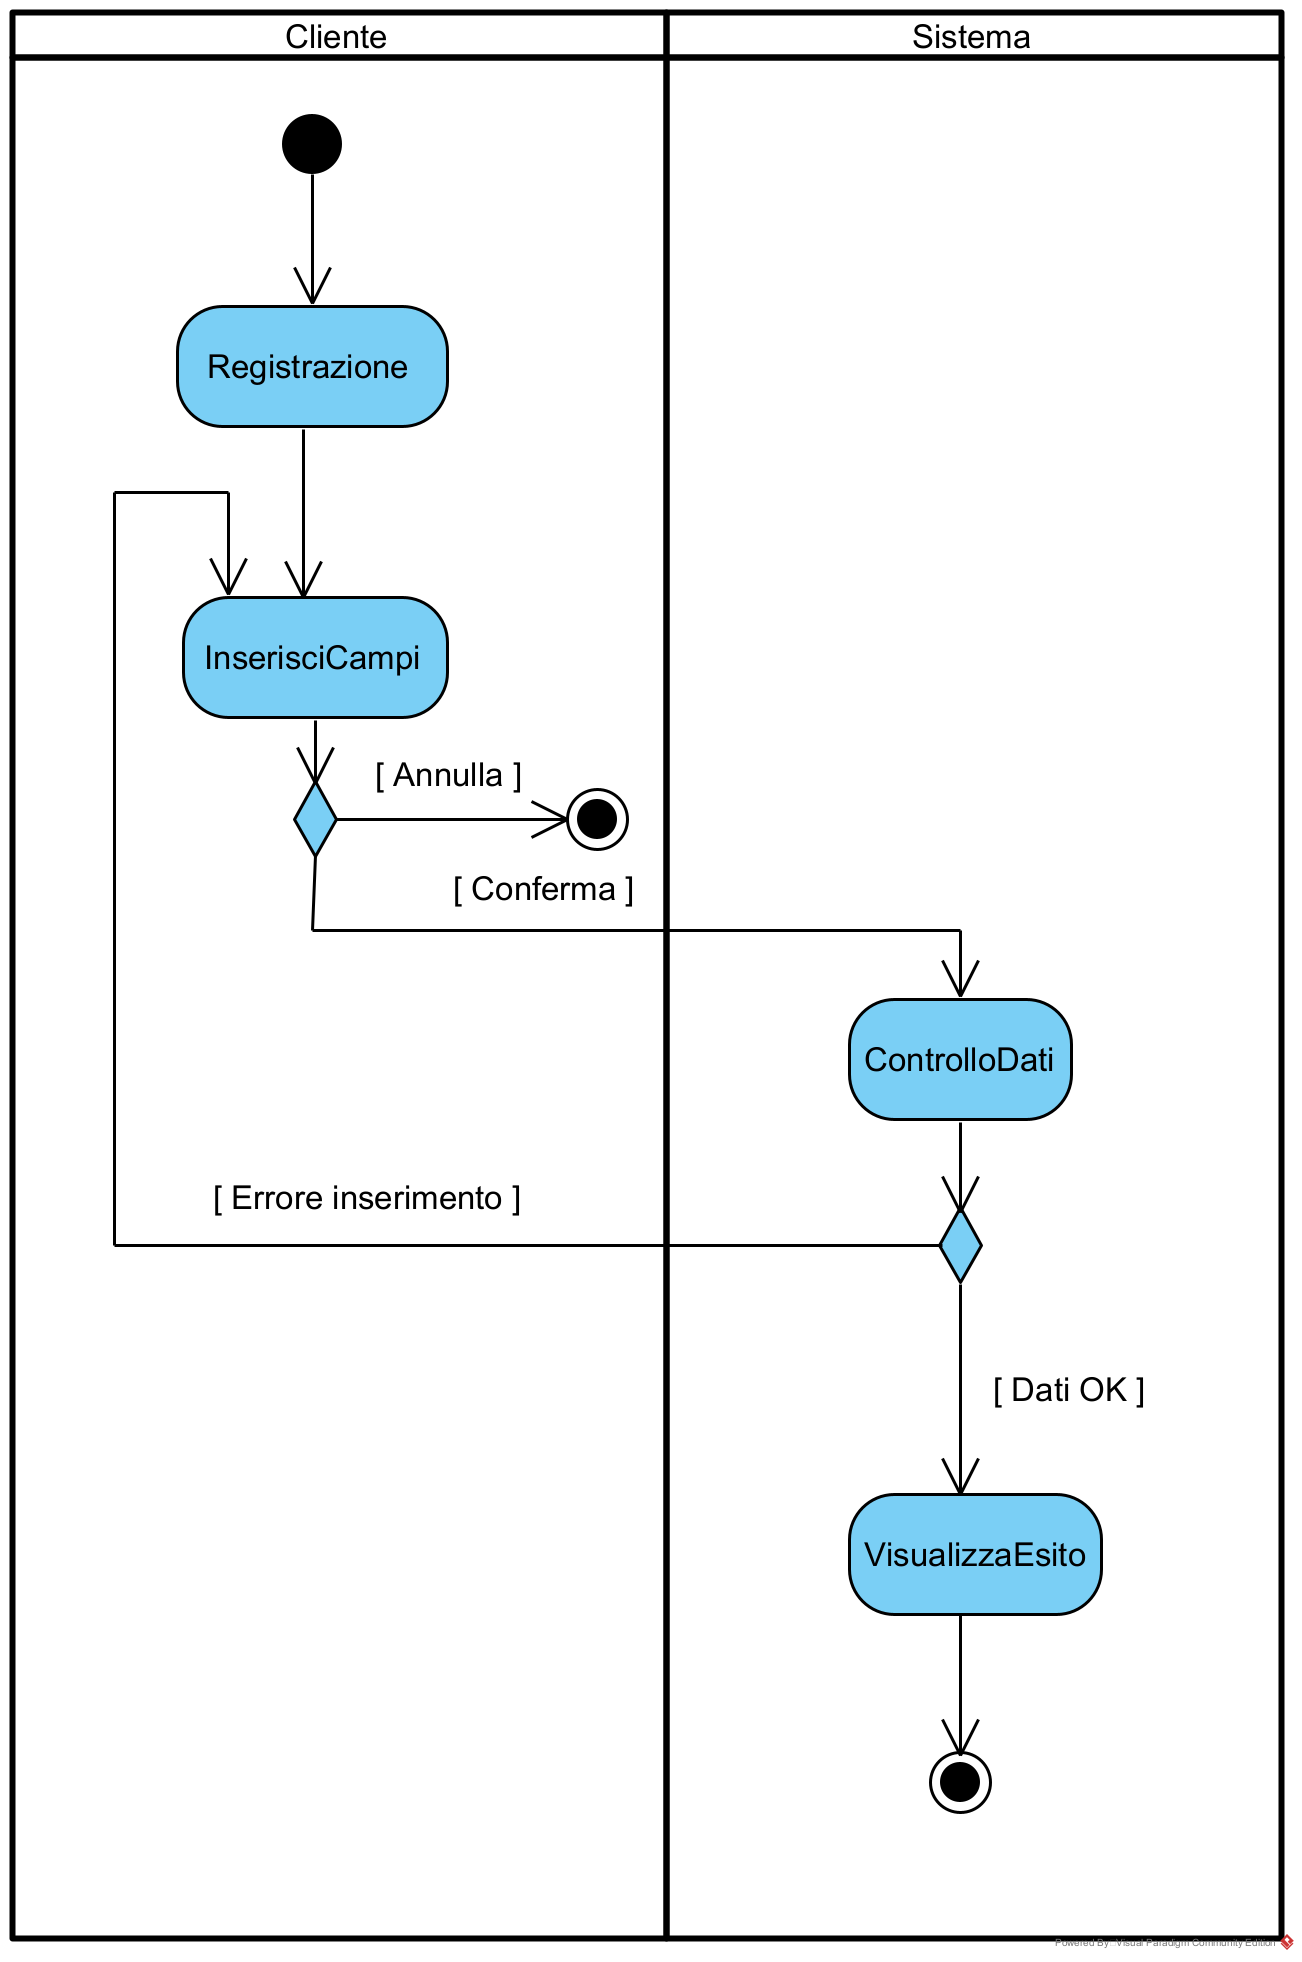
\includegraphics[width=\textwidth]{ActivityDiagram/ClienteRegistrazione}
\end{center}

\subsection{Acquisto}
\begin{center}
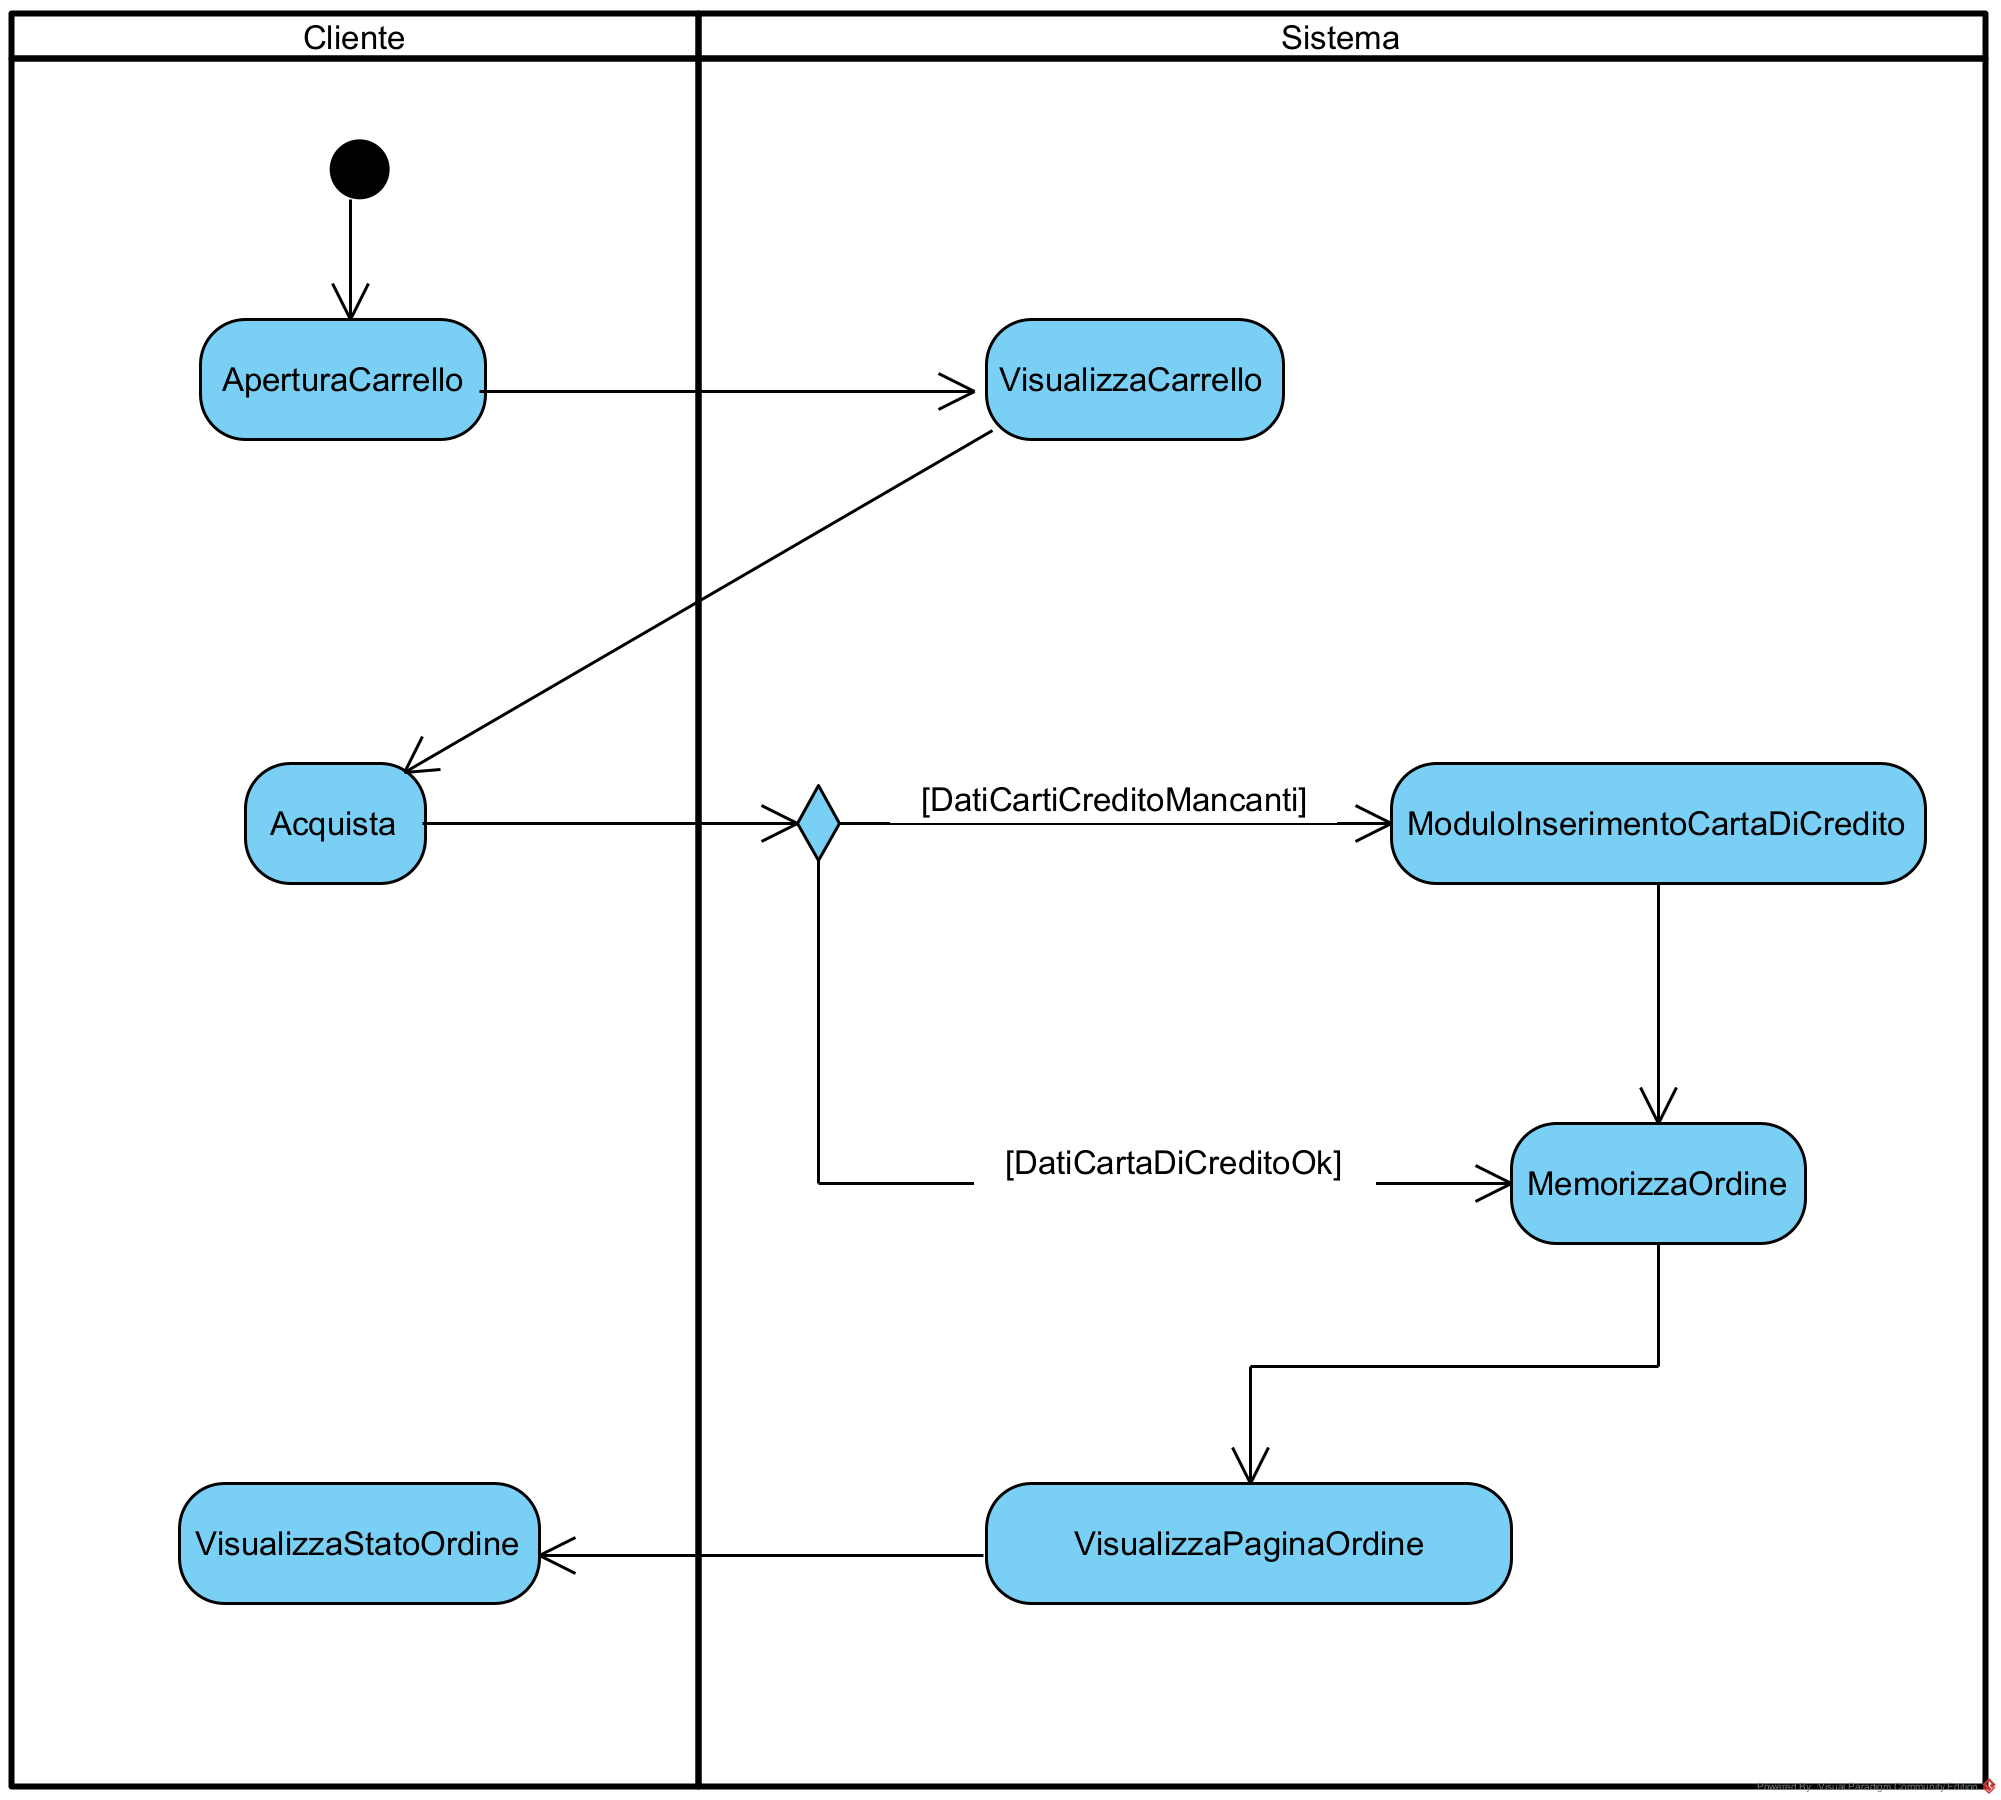
\includegraphics[width=\textwidth]{ActivityDiagram/ClienteAcquistoArticolo}
\end{center}

\subsection{Annullamento}
\begin{center}
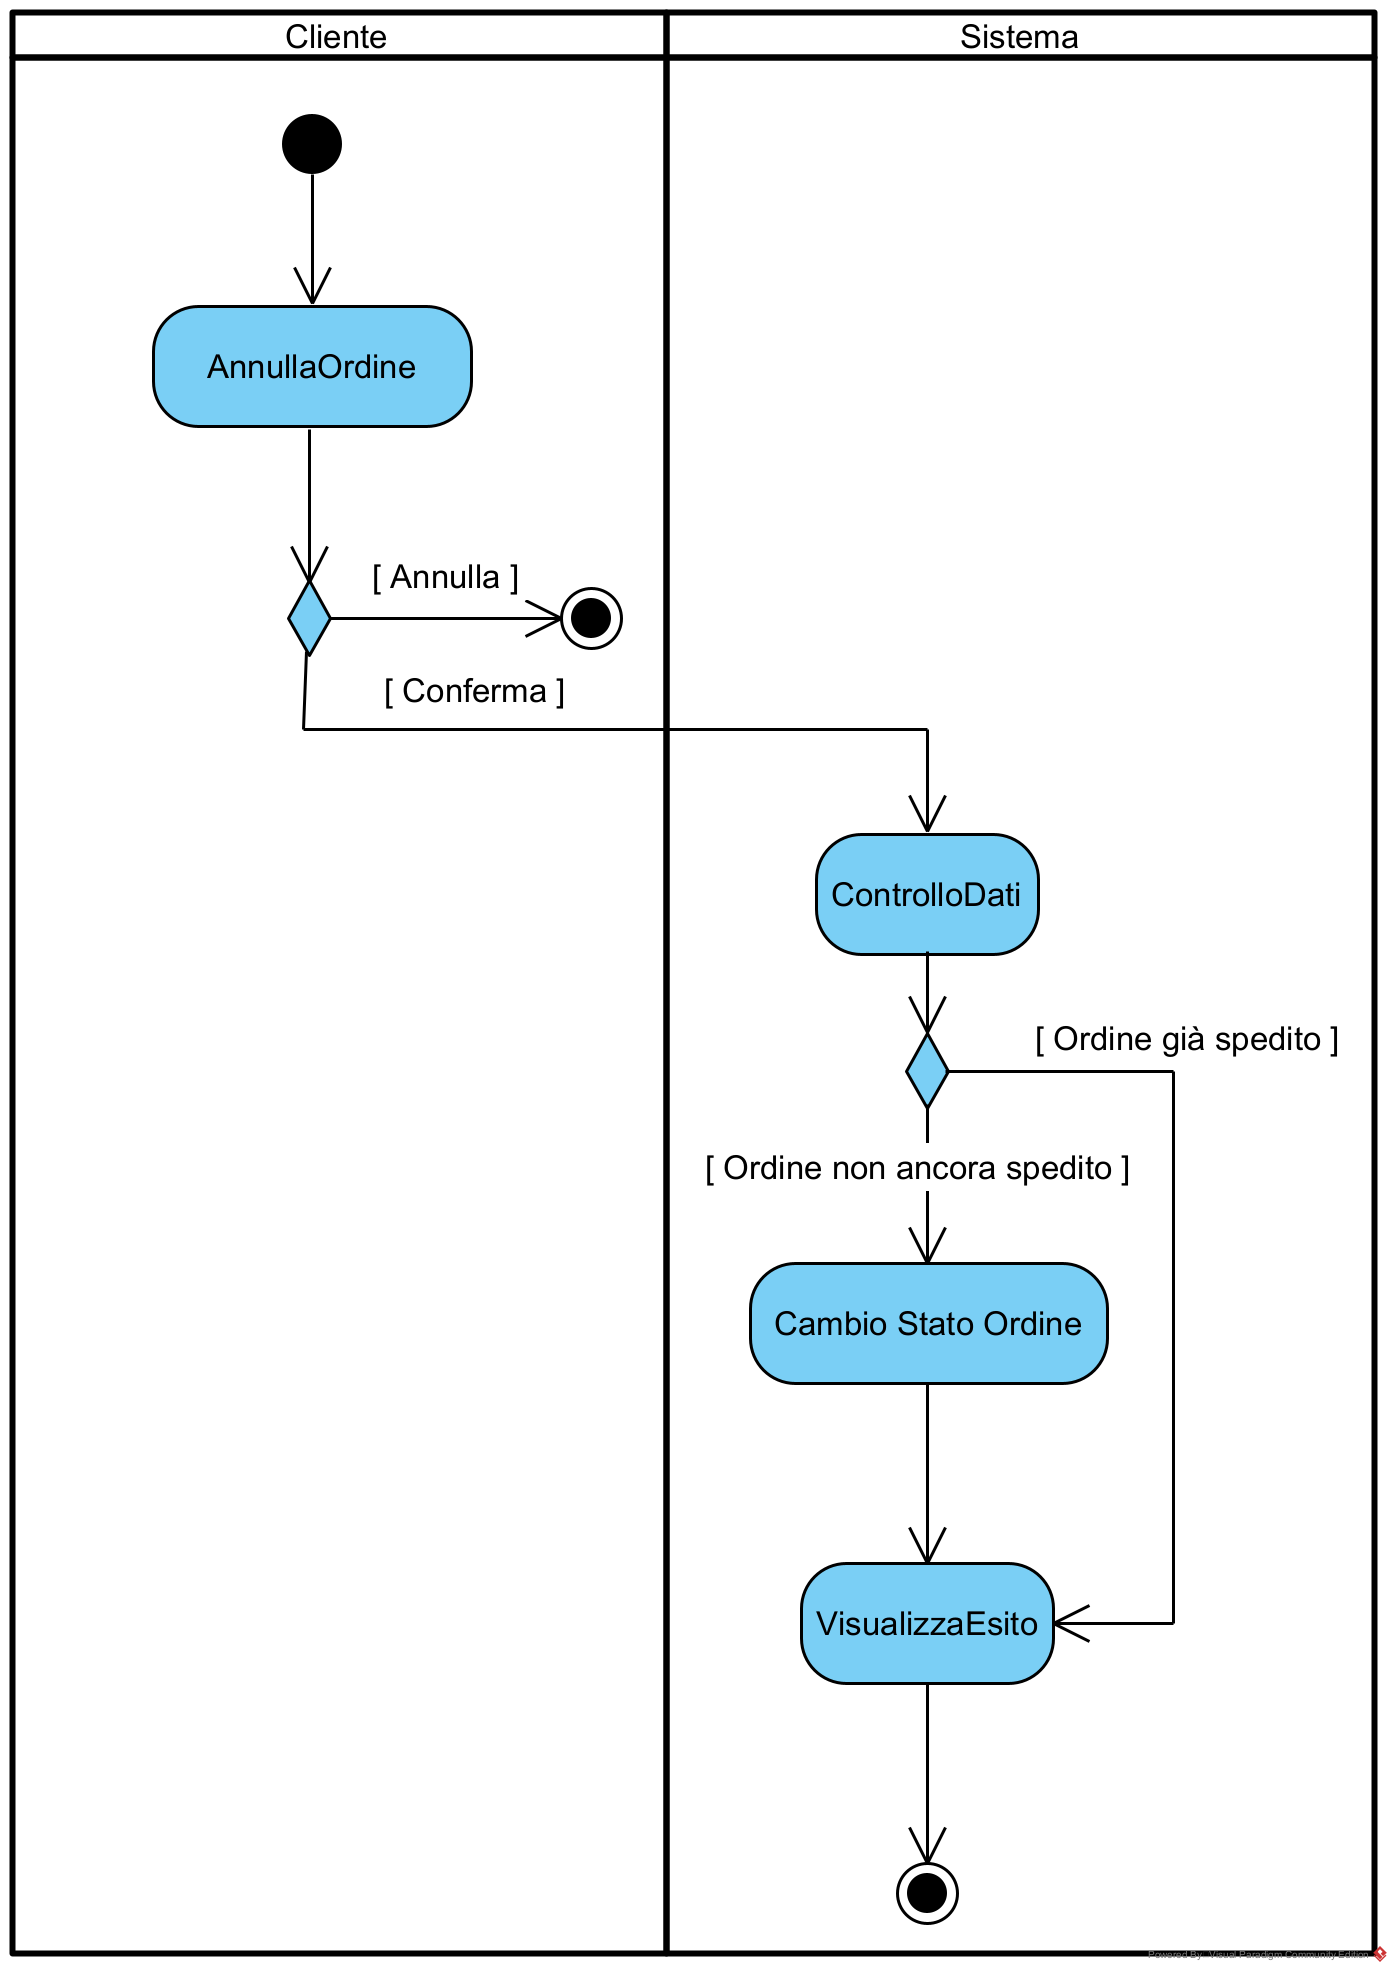
\includegraphics[width=\textwidth]{ActivityDiagram/ClienteAnnullamentoOrdine}
\end{center}

\subsection{Aggiunta al carrello}
\begin{center}
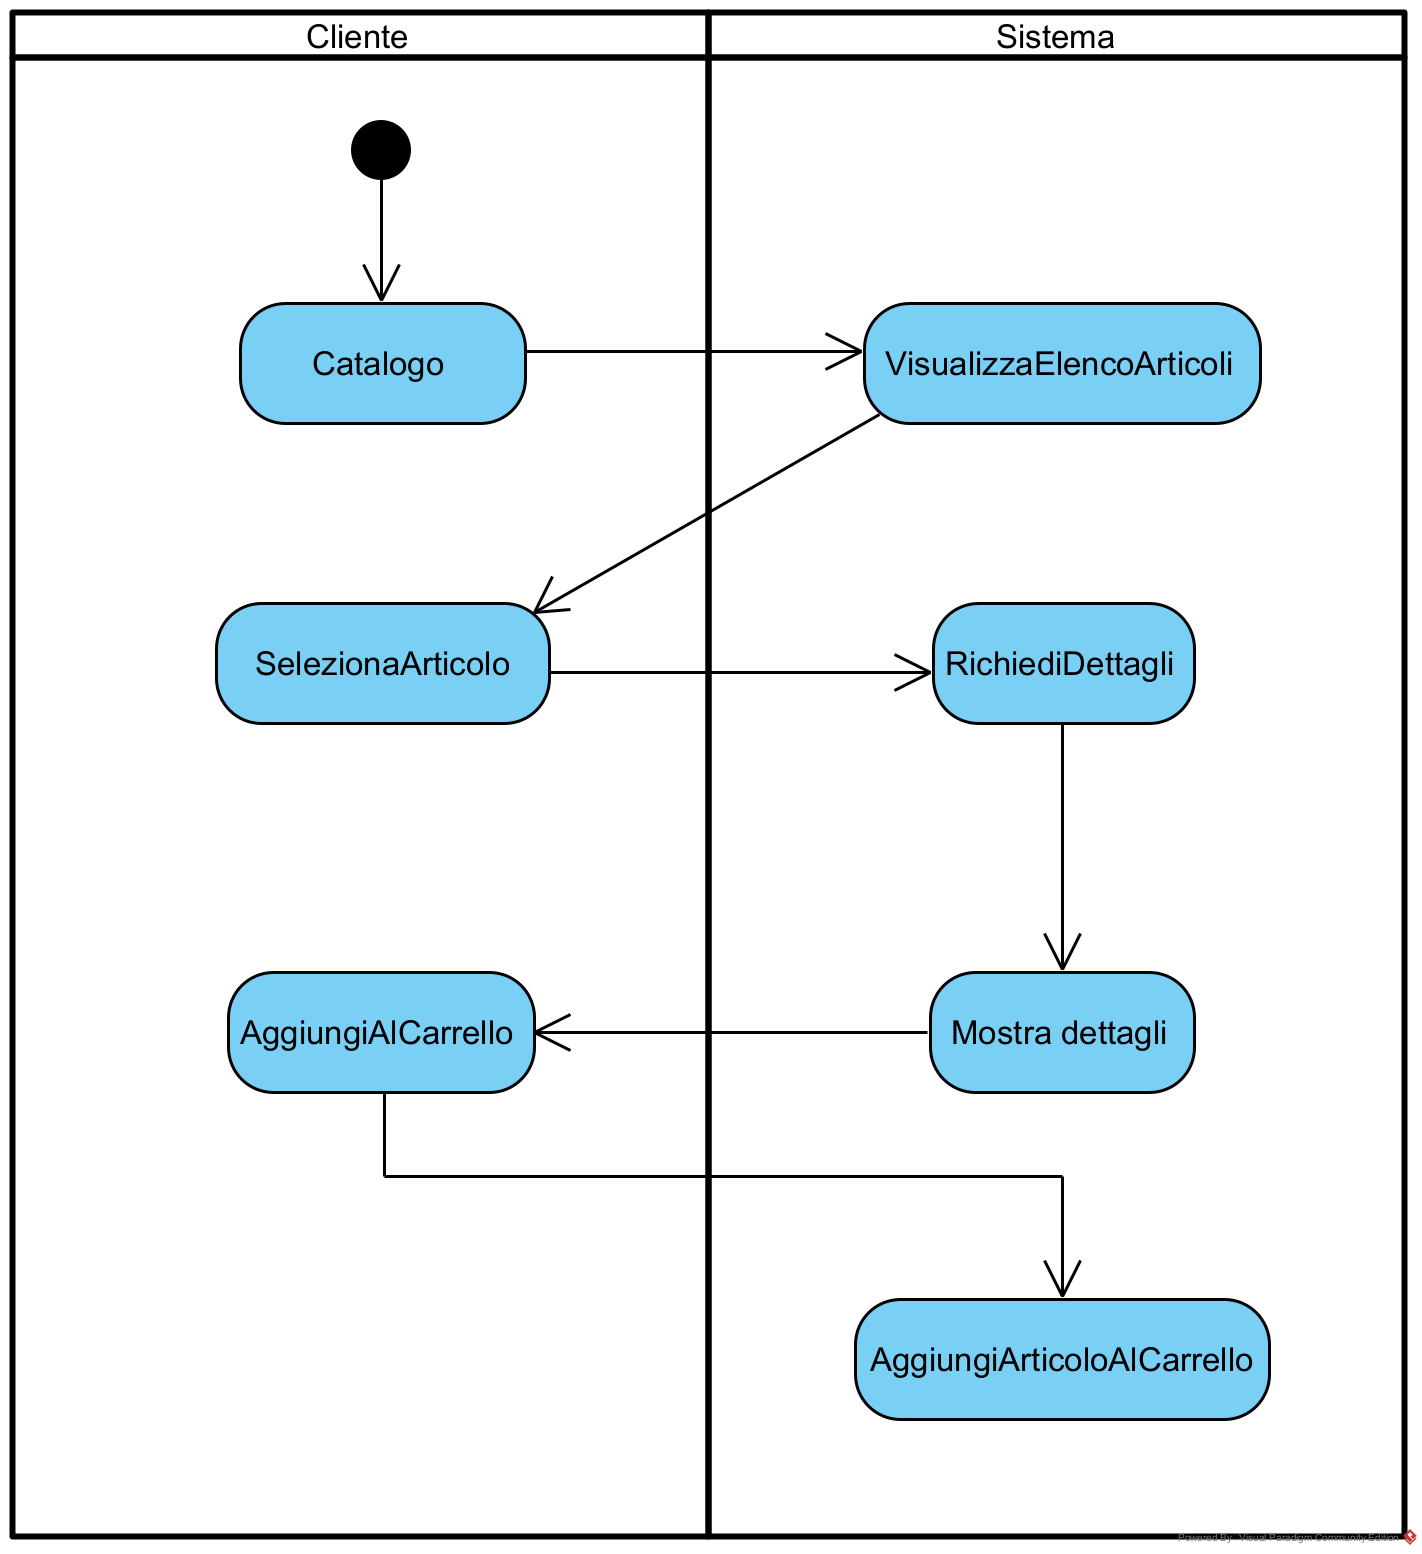
\includegraphics[width=\textwidth]{ActivityDiagram/ClienteAggiungeAlCarrello}
\end{center}

\subsection{Vendita}
\begin{center}
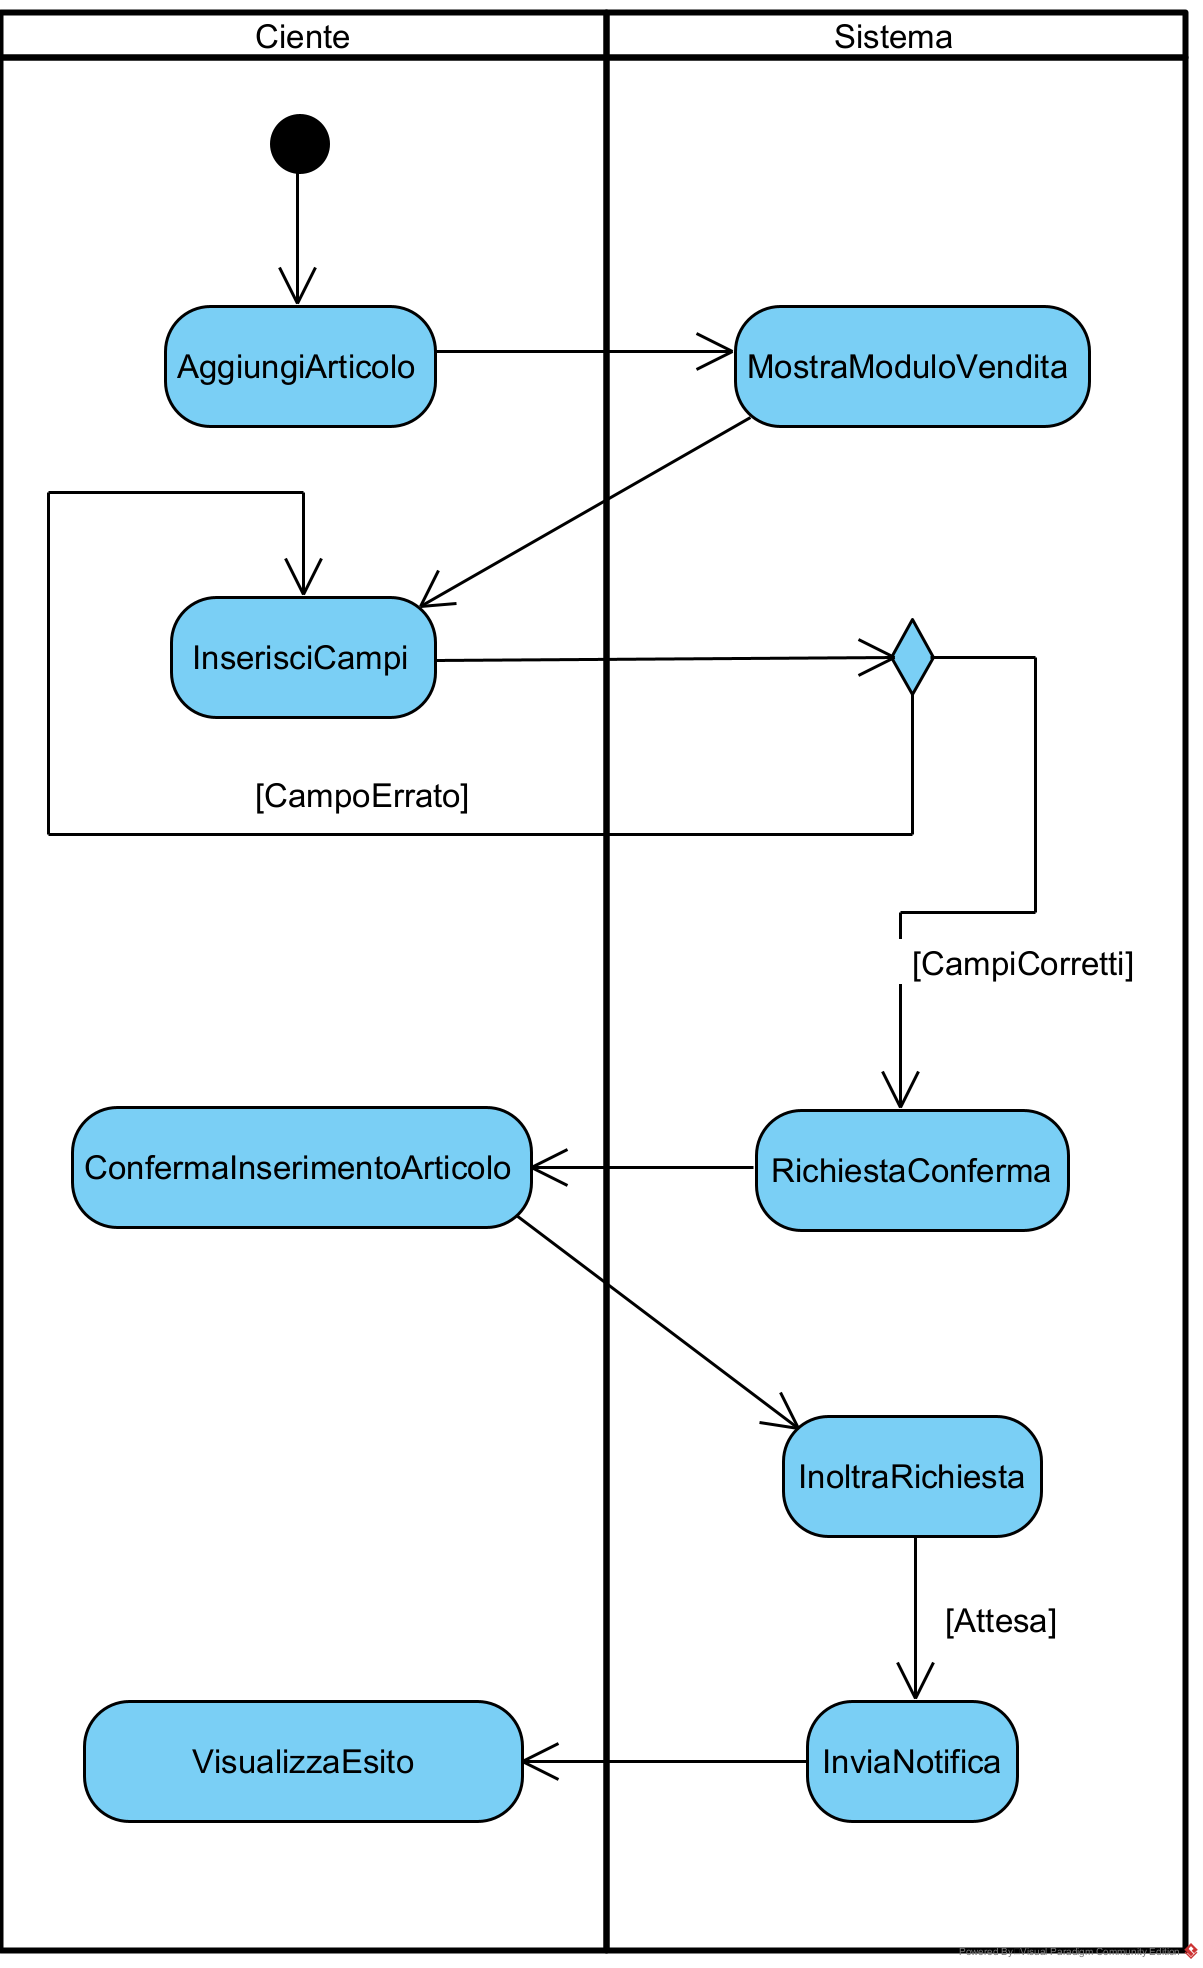
\includegraphics[height=0.95\textheight]{ActivityDiagram/ClienteVendita}
\end{center}

\subsection{Servizio Clienti}
\begin{center}
\includegraphics[width=\textwidth]{ActivityDiagram/ClienteCreazioneTicket}
\end{center}

\subsection{Spedizione Ordini}
\begin{center}
\includegraphics[width=\textwidth]{ActivityDiagram/MagazziniereSpedizioneOrdine}
\end{center}

\subsection{Autorizzazione vendita}
\begin{center}
\includegraphics[scale=1.3]{ActivityDiagram/CentralinistaAutorizzazioneVendita}
\end{center}

\subsection{Modifica personale}
\begin{center}
\includegraphics[scale=1.50]{ActivityDiagram/AmministratorePersonaleModificaDipendente}
\end{center}

\subsection{Modifica Catalogo}
\begin{center}
\includegraphics[scale=1.55]{ActivityDiagram/AmministratoreCatalogoModificaArticoloCatalogo}
\end{center}

\newpage
\section{Navigational Path}
\subsection{Cliente}
\begin{center}
\includegraphics[width=\textwidth]{NavigationalPath/Cliente}
\end{center}

\subsection{Centralinista}
\begin{center}
\includegraphics[height=300px]{NavigationalPath/Centralinista}
\end{center}

\subsection{Magazziniere}
\begin{center}
\includegraphics[height=300px]{NavigationalPath/Magazziniere}
\end{center}

\subsection{Amministratore Catalogo}
\begin{center}
\includegraphics[height=300px]{NavigationalPath/AmministratoreCatalogo}
\end{center}

\subsection{Amministratore Personale}
\begin{center}
\includegraphics[height=300px]{NavigationalPath/AmministratorePersonale}
\end{center}

\newpage
\section{Mock up}

\end{document}
